% =============================================================================
% Integrated Doctoral Thesis
%
% Title:  From Distributional Similarity to Causal Imbalance:
%         Circular Oversampling, Seed Selection, and a Controlled Degradation Study
%
% Author: Parsa Hajiannejad
%         Università degli Studi di Milano
% =============================================================================

\documentclass[12pt, a4paper, twoside, openright]{book}

% ---- Encoding & Language ---------------------------------------------------
\usepackage[utf8]{inputenc}
\usepackage[T1]{fontenc}
\usepackage[english]{babel}

% ---- Page Geometry ---------------------------------------------------------
\usepackage[
  top=3cm,
  bottom=3cm,
  inner=3.5cm,
  outer=2.5cm,
  headheight=15pt
]{geometry}

% ---- Fonts -----------------------------------------------------------------
\usepackage{mathpazo}
\usepackage{microtype}

% ---- Mathematics -----------------------------------------------------------
\usepackage{amsmath, amssymb, amsthm}
\usepackage{mathtools}
\usepackage{bm}

% ---- Graphics & Floats -----------------------------------------------------
\usepackage{graphicx}
\graphicspath{
  {../figures/circular_oversampling/}
  {../figures/causality/}
  {figures/}
}
\usepackage{float}
\usepackage{subcaption}
\usepackage[font=small, labelfont=bf]{caption}

% ---- Tables ----------------------------------------------------------------
\usepackage{booktabs}
\usepackage{tabularx}
\usepackage{multirow}
\usepackage{longtable}
\usepackage{array}
\newcolumntype{C}[1]{>{\centering\arraybackslash}p{#1}}

% ---- Algorithms ------------------------------------------------------------
\usepackage[ruled, vlined, linesnumbered]{algorithm2e}
\SetKwInput{KwInput}{Input}
\SetKwInput{KwOutput}{Output}
\SetKwInput{KwParam}{Parameters}
\SetAlFnt{\small}

% ---- Code listings ---------------------------------------------------------
\usepackage{listings}
\lstset{
  basicstyle=\ttfamily\small,
  keywordstyle=\bfseries\color{blue!70!black},
  commentstyle=\itshape\color{green!40!black},
  stringstyle=\color{red!60!black},
  numbers=left,
  numberstyle=\tiny,
  breaklines=true,
  frame=single,
  tabsize=4,
}

% ---- Colors ----------------------------------------------------------------
\usepackage{xcolor}
\definecolor{unimired}{RGB}{153,0,0}
\definecolor{linkblue}{RGB}{0,50,130}

% ---- Hyperlinks ------------------------------------------------------------
\usepackage[
  colorlinks=true,
  linkcolor=linkblue,
  citecolor=unimired,
  urlcolor=linkblue,
  bookmarks=true,
  bookmarksnumbered=true
]{hyperref}
\usepackage{url}
\pdfstringdefDisableCommands{%
  \def\kappa{}%
  \def\gamma{}%
  \def\sigma{}%
  \def\tau{}%
  \def\alpha{}%
  \def\mathrm#1{#1}%
  \def\max{}%
  \def\text#1{#1}%

}

% ---- Bibliography ----------------------------------------------------------
\usepackage{csquotes}
\usepackage[
  backend=biber,
  style=numeric-comp,
  sorting=nyt,
  maxnames=6,
  minnames=3,
  doi=false,
  isbn=false,
  url=false,
  eprint=false
]{biblatex}
\addbibresource{references.bib}

% ---- Header / Footer -------------------------------------------------------
\usepackage{fancyhdr}
\pagestyle{fancy}
\fancyhf{}
\fancyhead[LE]{\nouppercase{\leftmark}}
\fancyhead[RO]{\nouppercase{\rightmark}}
\fancyfoot[C]{\thepage}
\renewcommand{\headrulewidth}{0.4pt}
\renewcommand{\footrulewidth}{0pt}

% ---- Theorem Environments --------------------------------------------------
\theoremstyle{plain}
\newtheorem{theorem}{Theorem}[chapter]
\newtheorem{proposition}[theorem]{Proposition}
\newtheorem{lemma}[theorem]{Lemma}
\newtheorem{corollary}[theorem]{Corollary}
\theoremstyle{definition}
\newtheorem{definition}{Definition}[chapter]
\newtheorem{remark}{Remark}[chapter]

% ---- Spacing ---------------------------------------------------------------
\usepackage{setspace}
\onehalfspacing

% ---- Miscellaneous ---------------------------------------------------------
\usepackage{enumitem}
\usepackage{xspace}
\usepackage{pdfpages}
\usepackage{appendix}
\usepackage{pifont}
\newcommand{\starmark}{\ding{72}}

% ---- Part style (add "Part" label) -----------------------------------------
\usepackage{titlesec}
% Give parts a clear "Part X — Title" header
\titleformat{\part}[display]
  {\normalfont\huge\bfseries\centering}
  {\partname\ \thepart}{20pt}{\Huge}

% ---- Custom Commands -------------------------------------------------------
\newcommand{\thesistitle}{%
  From Distributional Similarity to Causal Imbalance:
  Circular Oversampling, Seed Selection, and a Controlled Degradation Study}
\newcommand{\authorname}{Parsa Hajiannejad}
\newcommand{\R}{\mathbb{R}}
\newcommand{\N}{\mathbb{N}}
\newcommand{\E}{\mathbb{E}}
\newcommand{\Var}{\mathrm{Var}}
\newcommand{\Cov}{\mathrm{Cov}}
\newcommand{\IR}{\mathrm{IR}}
\newcommand{\TV}{\operatorname{TV}}
\newcommand{\OVL}{\operatorname{OVL}}
%%% \newcommand{\NHOP}{\operatorname{NHOP}}  % REMOVED — NHOP no longer in thesis
\newcommand{\HI}{\operatorname{HI}}
\newcommand{\BC}{\operatorname{BC}}
\newcommand{\KL}{\operatorname{KL}}
\newcommand{\JS}{\operatorname{JS}}
%%% \newcommand{\nhop}{NHOP\xspace}  % REMOVED
\newcommand{\vx}{\bm{x}}
\newcommand{\vy}{\bm{y}}
\newcommand{\vz}{\bm{z}}
\newcommand{\vc}{\bm{c}}
\newcommand{\vmu}{\bm{\mu}}
\newcommand{\vg}{\bm{g}}
\DeclareMathOperator*{\argmax}{arg\,max}
\DeclareMathOperator*{\argmin}{arg\,min}

% ============================================================================
%  DOCUMENT
% ============================================================================
\begin{document}

% ---- Front Matter ----------------------------------------------------------
\frontmatter
\pagenumbering{roman}

% Title page
\begin{titlepage}
\centering
\vspace*{2cm}
{\Large Università degli Studi di Milano\\
Laurea Magistrale in Computer Science\par}
\vspace{3cm}
{\huge\bfseries \thesistitle\par}
\vspace{2cm}
{\Large\itshape \authorname\par}
\vfill
{\large Academic Year 2024--2025\par}
\end{titlepage}
\cleardoublepage

% ---- Abstract --------------------------------------------------------------
% =============================================================================
% Abstract
% =============================================================================
\chapter*{Abstract}
\addcontentsline{toc}{chapter}{Abstract}
\markboth{Abstract}{Abstract}

This thesis presents three interlinked contributions forming a methodological pipeline for class imbalance in binary classification.

\medskip\noindent
We propose a four-stage geometry-preserving seed-selection pipeline (K-means clustering, PCA projection, composite Bhattacharyya Coefficient + Jensen--Shannon Divergence + Average Geometric--Topological Preservation (AGTP) + smoothness scoring) that improves downstream F1 by $+0.025$ over random-seed baselines.

\medskip\noindent
We then develop three circle-based oversampling algorithms that replace SMOTE (Synthetic Minority Over-sampling Technique) line-segment generation with disk generation in PCA-projected space: GVM-CO (Gravity-biased Von Mises Circular Oversampling), which biases angular sampling toward minority cluster gravity centers using a Von Mises distribution; LRE-CO (Local Region Estimation), which enforces Voronoi-cell certainty constraints; and LS-CO (Layered Segmental), which applies concentric-ring angular segmentation. Evaluated on 14 KEEL/UCI benchmark datasets, LRE-CO achieves the best mean F1 rank (6.14/13) across all methods.

\medskip\noindent
Finally, a controlled degradation-and-recovery causal study confirms that class imbalance \emph{per se} degrades performance monotonically, with a non-linear threshold at imbalance ratio $\IR \approx 2$. No oversampler achieves full recovery; GVM-CO and K-Means SMOTE reach 98.4\% of balanced AUC, with a residual gap attributable to irreducible information loss.

\medskip

\noindent\textbf{Keywords:} class imbalance, oversampling, distributional similarity, circular generation, Von Mises distribution, causal analysis, degradation study, seed selection.

\cleardoublepage

% ---- Table of Contents -----------------------------------------------------
\tableofcontents
\cleardoublepage

\listoffigures
\cleardoublepage

\listoftables
\cleardoublepage

% ---- Main Matter -----------------------------------------------------------
\mainmatter
\pagenumbering{arabic}

% ============================================================================
\part{Foundations}
\label{part:foundations}
% ============================================================================

% =============================================================================
% Chapter 1 -- Unified Introduction
% =============================================================================

\chapter{Introduction}
\label{ch:introduction}

\section{Motivation and Research Programme}
\label{sec:intro:motivation}

Class imbalance --- when one class in a binary dataset is vastly underrepresented --- degrades classifier performance precisely in the domains where correctness matters most: fraud detection~\cite{dal2014learned}, medical diagnosis~\cite{mazurowski2008training}, intrusion detection~\cite{tavallaee2009detailed}, and industrial defect detection~\cite{wang2016automatically}.
When the majority class dominates the empirical risk, the classifier learns a boundary biased toward the majority at the expense of the minority~\cite{japkowicz2002class, he2009learning}.

The most widely adopted remedy is oversampling.
SMOTE~\cite{chawla2002smote} generates synthetic minority samples by linearly interpolating between a seed and one of its $k$-nearest neighbors:
\begin{equation}
  \vx_{\mathrm{new}} = \vx_i + \lambda \cdot (\vx_j - \vx_i), \quad \lambda \sim \mathcal{U}(0,1).
  \label{eq:smote}
\end{equation}
Despite over 10{,}000 citations and dozens of variants~\cite{fernandez2018smote}, SMOTE confines all synthetic samples to a \emph{one-dimensional line segment}, ignoring the 2-D neighbourhood structure of each minority pair.
This leads to linear artefacts, class-overlap amplification near boundaries, and noise sensitivity~\cite{han2005borderline, batista2004study}.

Two open problems drive this thesis:
\begin{enumerate}
  \item \textbf{No principled seed selection.} Neither SMOTE nor any variant uses a formally motivated criterion for which minority instances should serve as seeds.
  \item \textbf{The causal question is unresolved.} Every oversampling paper assumes imbalance degrades performance, but no controlled study has isolated the effect of imbalance itself from confounding factors such as reduced sample size.
\end{enumerate}

Part~II addresses problem~1 with a geometry-preserving seed selection pipeline using the Bhattacharyya Coefficient~\cite{bhattacharyya1943measure} and complementary metrics, together with three circular oversampling algorithms (Parts~II--III) that replace SMOTE's line segment with a disk.
Part~IV addresses problem~2 with a controlled degradation-and-recovery study using uniform random minority removal to isolate pure imbalance from distributional shift.

\section{Research Questions}
\label{sec:intro:rqs}

This thesis addresses seven research questions spanning the two main works:

\begin{description}[leftmargin=!, labelwidth=\widthof{\textbf{RQ7:}}]
  \item[\textbf{RQ1}] Can a geometry-preserving seed selection criterion, based on the Bhattacharyya Coefficient and complementary metrics, improve the quality of oversampled minority data?
  \item[\textbf{RQ2}] Can circle-based generation outperform linear interpolation for oversampling imbalanced datasets?
  \item[\textbf{RQ3}] Does gravity-biased angular sampling via Von Mises distributions improve synthetic sample quality?
  \item[\textbf{RQ4}] Does the choice of seed selection strategy impact the quality of oversampled data?
  \item[\textbf{RQ5}] Does progressive class imbalance monotonically degrade classifier performance, or is there a threshold effect?
  \item[\textbf{RQ6}] Can oversampling methods fully recover balanced-dataset performance after degradation?
  \item[\textbf{RQ7}] Is performance loss caused by imbalance \emph{per se}, or primarily by information loss from a smaller minority sample?
\end{description}

\section{Contributions}
\label{sec:intro:contributions}

The specific contributions of this thesis, labeled C1--C5, are as follows:

\begin{enumerate}[label=\textbf{C\arabic*.}, leftmargin=*, itemsep=4pt]
  \item \textbf{Geometry-preserving seed selection} (Part~II): a composite criterion combining the Bhattacharyya Coefficient (marginal fidelity), JSD (distributional divergence), AGTP (geometric-topological preservation), and $Z$ (smoothness regulariser); a four-stage pipeline with cluster-proportional stratified sampling; and a PCA ablation study.

  \item \textbf{GVM-CO} (Part~III): gravity scoring framework (Spread, Area, Density, Sparsity, Gravity score $g_c$, Gravity center $\vg_c$), Von Mises angular biasing with concentration $\kappa = \kappa_{\max} \cdot s_c^{\gamma}$, cross-cluster and full-dataset clustering variants.

  \item \textbf{LRE-CO and LS-CO} (Part~III): LRE-CO provides Voronoi-constrained generation with certainty threshold and rejection sampling within the disk-Voronoi intersection. LS-CO provides layered segmental generation with concentric rings and angular segments, generic and cluster-based variants.

  \item \textbf{Controlled degradation-recovery experimental protocol} (Part~IV): uniform random minority removal ensuring no distributional bias; leakage-safe four-rule cross-validation protocol preventing the three main forms of data leakage in oversampling studies~\cite{kaufman2012leakage, cawley2010over}.

  \item \textbf{Empirical causal evidence for class imbalance} (Part~IV): characterization of the degradation signature across six metrics, five classifiers, and ten datasets; comparative recovery analysis of seven oversampling methods; evidence for a non-linear threshold at $\IR \approx 2$; and quantification of the irreducible information-loss gap.
\end{enumerate}

\section{Thesis Organization}
\label{sec:intro:organization}

\textbf{Part~I} (Chapters~2--3) provides background and a literature review.
\textbf{Part~II} (Chapter~4) presents the seed selection pipeline.
\textbf{Part~III} (Chapters~5--9) presents the three circular algorithms with results and ablation.
\textbf{Part~IV} (Chapters~10--14) presents the causal study: protocol, degradation, recovery, and discussion.
\textbf{Part~V} (Chapter~15) synthesises all contributions, answers RQ1--RQ7, and outlines future directions.


% =============================================================================
% Chapter 2 -- Background
% =============================================================================

\chapter{Background}
\label{ch:background}

This chapter provides the theoretical foundations upon which the contributions of this thesis are built:
the class imbalance problem and why standard classifiers fail under it, evaluation metrics for imbalanced data, SMOTE's geometric limitation, clustering methods, cross-validation, statistical hypothesis testing for multi-method comparison, the Von Mises distribution, and distributional similarity measures.

% ============================================================================
\section{The Class Imbalance Problem}
\label{sec:bg:imbalance}

\subsection{Definition and Quantification}

\begin{definition}[Imbalance Ratio]
\label{def:ir}
The \emph{imbalance ratio} (IR) of a binary dataset is defined as
\begin{equation}
  \IR = \frac{n_{\mathrm{maj}}}{n_{\mathrm{min}}},
  \label{eq:ir}
\end{equation}
where $n_{\mathrm{maj}}$ is the number of majority-class instances and $n_{\mathrm{min}}$ is the number of minority-class instances.
An IR of 1.0 indicates perfect balance; larger values indicate increasing imbalance.
\end{definition}

Datasets with $\IR < 3$ are considered mildly imbalanced, those with $3 \leq \IR < 9$ are moderately imbalanced, and those with $\IR \geq 9$ are highly imbalanced~\cite{fernandez2018learning}.
Some applications feature extreme imbalance with $\IR > 100$.

\subsection{Why Standard Classifiers Fail}

Standard algorithms minimize the empirical risk:
\begin{equation}
  \hat{R}(h) = \frac{1}{n}\sum_{i=1}^n \ell(h(\vx_i), y_i),
  \label{eq:empirical_risk}
\end{equation}
where $\ell$ is the loss function.
When classes are imbalanced, the majority class contributes disproportionately.
A classifier that always predicts majority achieves $\IR/(1+\IR)$ accuracy while having zero sensitivity for the minority~\cite{japkowicz2002class}.

This problem manifests specifically across classifier families:
\begin{itemize}[leftmargin=*]
  \item \textbf{Decision trees:} Information gain and Gini impurity are dominated by the majority class~\cite{cieslak2012hellinger}.
  \item \textbf{SVMs:} The separating hyperplane is pushed toward the minority region~\cite{akbani2004applying}.
  \item \textbf{Neural networks:} The gradient of the cross-entropy loss is dominated by majority examples~\cite{buda2018systematic}.
  \item \textbf{$k$-Nearest Neighbours:} The neighbourhood of a minority instance is likely to contain a majority of majority points~\cite{zhang2003knearest}.
\end{itemize}

\subsection{Real-World Manifestations}

Table~\ref{tab:bg:realworld} illustrates the prevalence of class imbalance across application domains.

\begin{table}[ht]
\centering
\caption{Examples of class imbalance in real-world applications.}
\label{tab:bg:realworld}
\begin{tabular}{llc}
\toprule
\textbf{Domain} & \textbf{Task} & \textbf{Typical IR} \\
\midrule
Finance & Credit card fraud detection & 500:1--1000:1 \\
Medicine & Rare disease diagnosis & 50:1--200:1 \\
Manufacturing & Defect detection & 10:1--100:1 \\
Cybersecurity & Intrusion detection & 100:1--10{,}000:1 \\
Oil \& Gas & Oil spill detection & 20:1--500:1 \\
Text mining & Spam detection & 5:1--20:1 \\
Bioinformatics & Protein function prediction & 10:1--100:1 \\
\bottomrule
\end{tabular}
\end{table}

% ============================================================================
\section{Evaluation Metrics for Imbalanced Data}
\label{sec:bg:metrics}

Standard accuracy is misleading when classes are imbalanced; a majority-only predictor achieves $\IR/(1+\IR)$ accuracy at zero minority-class recall.
Table~\ref{tab:bg:metrics} summarises the six metrics used throughout this thesis; all are computed from the entries of the binary confusion matrix (TP, FP, FN, TN).

\begin{table}[ht]
\centering
\caption{Evaluation metrics for imbalanced classification used in this thesis.}
\label{tab:bg:metrics}
\small
\begin{tabular}{llp{5.8cm}}
\toprule
\textbf{Metric} & \textbf{Formula} & \textbf{Key property for imbalanced data} \\
\midrule
Sensitivity (Recall) & $\mathrm{TP}/(\mathrm{TP}+\mathrm{FN})$ & Measures minority-class coverage; collapses to 0 under naive majority predictor \\
Specificity          & $\mathrm{TN}/(\mathrm{TN}+\mathrm{FP})$ & Measures majority-class accuracy \\
$F_1$                & $2\mathrm{TP}/(2\mathrm{TP}+\mathrm{FP}+\mathrm{FN})$ & Harmonic mean of precision and recall~\cite{sokolova2009systematic} \\
G-Mean               & $\sqrt{\text{Sens.} \times \text{Spec.}}$ & Zero if either class is entirely missed~\cite{kubat1997addressing} \\
Balanced Accuracy    & $(\text{Sens.}+\text{Spec.})/2$ & Trivial predictor achieves 0.5~\cite{brodersen2010balanced} \\
AUC                  & $\int_0^1 \text{TPR}\,d(\text{FPR})$ & Threshold-free; equals $P(\hat{s}^+>\hat{s}^-)$~\cite{fawcett2006introduction} \\
\bottomrule
\end{tabular}
\end{table}

% ============================================================================
\section{SMOTE and Its Limitations}
\label{sec:bg:smote}

SMOTE~\cite{chawla2002smote} generates synthetic samples by linearly interpolating between a minority seed $\vx_i$ and a randomly chosen $k$-NN $\vx_j$:
\begin{equation}
  \vx_{\mathrm{new}} = \vx_i + \lambda(\vx_j - \vx_i), \quad \lambda \sim \mathcal{U}(0,1).
  \label{eq:smote_bg}
\end{equation}
This places all synthetic samples on line segments in the minority class, generating a $1$-D submanifold of the $d$-dimensional feature space.
The geometric limitation motivates the circular generation framework of Part~IV.

% ============================================================================
\section{Clustering and Cross-Validation}
\label{sec:bg:clustering}

Two clustering algorithms are used in the seed selection and algorithm components of this thesis.
\textbf{$K$-means}~\cite{macqueen1967some} with $k$-means++ initialization~\cite{arthur2007kmeans} partitions the minority class into $K$ convex clusters by minimizing total within-cluster variance; its spherical cluster assumption aligns well with the circular geometry of our generation regions.
\textbf{HAC} (hierarchical agglomerative clustering with Ward's linkage~\cite{murtagh2012algorithms}) is used as a comparison baseline in the ablation of Chapter~\ref{ch:ablation}; it captures non-spherical shapes but produces unbalanced clusters on small minority sets.

For evaluation, stratified $k$-fold cross-validation~\cite{kohavi1995study} is used throughout to preserve class ratios per fold.
When evaluating oversampling, synthesis must be applied \emph{inside the training partition of each fold only}; applying it before splitting introduces data leakage and produces optimistically biased estimates~\cite{kaufman2012leakage, cawley2010over}.
The four-rule leakage-safe protocol used in Part~V is described in Section~\ref{sec:setup:leakage}.

% ============================================================================
\section{Statistical Hypothesis Testing for Method Comparison}
\label{sec:bg:statistics}

\subsection{Friedman Test}

The Friedman test~\cite{friedman1937use} is a non-parametric test for comparing $K$ algorithms across $N$ datasets.
Let $r_i^j$ denote the rank of algorithm $j$ on dataset $i$.
The Friedman statistic is:
\begin{equation}
  F_F = \frac{12N}{K(K+1)} \left[ \sum_j \bar{r}_j^2 - \frac{K(K+1)^2}{4} \right],
  \label{eq:friedman}
\end{equation}
where $\bar{r}_j$ is the average rank of algorithm $j$.
Under the null hypothesis that all algorithms are equivalent, $F_F$ follows a $\chi^2$ distribution with $K-1$ degrees of freedom.

\subsection{Holm's Procedure for Post-Hoc Comparisons}

When the Friedman test rejects the null, Holm's step-down procedure~\cite{holm1979simple} controls the family-wise error rate for pairwise comparisons between a control method and all others.
Pairwise comparisons use the Wilcoxon signed-rank test~\cite{wilcoxon1945individual}.

\subsection{Nemenyi Critical Difference Diagrams}

Nemenyi critical difference (CD) diagrams~\cite{demsar2006statistical} provide a visual summary.
The critical difference for a test at significance level $\alpha$ with $K$ algorithms and $N$ datasets is:
\begin{equation}
  \mathrm{CD} = q_\alpha \sqrt{\frac{K(K+1)}{6N}},
  \label{eq:cd}
\end{equation}
where $q_\alpha$ is the critical value from the studentised range distribution.
Algorithms whose average ranks differ by less than CD are connected by a horizontal bar in the diagram, indicating no statistically significant difference.

% ============================================================================
\section{The Von Mises Distribution}
\label{sec:bg:vonmises}

The Von Mises distribution is the natural analogue of the Gaussian distribution on the unit circle.
A random angle $\theta \sim \mathrm{VM}(\mu, \kappa)$ has probability density function:
\begin{equation}
  p(\theta) = \frac{\exp(\kappa \cos(\theta - \mu))}{2\pi I_0(\kappa)},
  \label{eq:vonmises}
\end{equation}
where $\mu \in [0, 2\pi)$ is the mean direction, $\kappa \geq 0$ is the concentration parameter, and $I_0(\kappa) = \frac{1}{2\pi}\int_0^{2\pi} e^{\kappa\cos\theta}\,d\theta$ is the modified Bessel function of order zero.

When $\kappa = 0$, the distribution is uniform on $[0, 2\pi)$; as $\kappa \to \infty$, the distribution concentrates around $\mu$.
The Von Mises distribution is used in GVM-CO (Chapter~\ref{ch:proposed_methods}) to bias angular sampling toward the gravity center of each minority cluster, with $\kappa$ computed from the cluster's gravity score~\cite{mardia2000directional}.

% ============================================================================
\section{Distributional Similarity Measures}
\label{sec:bg:distrib_similarity}

This section surveys the distributional similarity measures used in the seed selection criterion of Part~II.

\subsection{Histogram Intersection}
\label{sec:bg:histogram_intersection}

Histogram intersection was introduced by Swain and Ballard~\cite{swain1991color} for colour-based image retrieval.
Given two histograms $h$ and $h'$ with the same bins, the intersection is $\HI(h,h') = \sum_b \min(h_b, h'_b)$.
When histograms record raw counts, the result depends on sample sizes $n$ and $m$ unless explicitly normalised.
Swain and Ballard normalise by $\min(\sum h_b, \sum h'_b)$, which introduces asymmetry when $n \neq m$.
The Bhattacharyya Coefficient (below) avoids this by using normalised proportions and a geometric-mean overlap, yielding a symmetric, sample-size-invariant score.

\subsection{Bhattacharyya Coefficient}

The Bhattacharyya coefficient~\cite{bhattacharyya1943measure} is $\BC(P,Q) = \sum_b \sqrt{p_b q_b} \in [0,1]$.
It is symmetric and bounded but uses the geometric mean rather than the minimum, making it less sensitive to partial mismatches.
The relationship $\BC \leq 1 - \TV^2/2$ holds, but $\BC$ does not equal $1 - \TV$ in general.

\subsection{Maximum Mean Discrepancy (MMD)}

MMD~\cite{gretton2012kernel} is an integral probability metric associated with a reproducing kernel Hilbert space.
It requires choice of a kernel and bandwidth and is quadratic in sample size ($O(n^2)$), limiting scalability.
MMD lacks a direct percentage interpretation.

\subsection{Jensen--Shannon Divergence (JSD)}

JSD~\cite{lin1991divergence} symmetrises KL divergence via the mixture $M = (P+Q)/2$:
\begin{equation}
  \JS(P,Q) = \frac{1}{2}\KL(P\|M) + \frac{1}{2}\KL(Q\|M) \in [0, \log 2].
  \label{eq:jsd}
\end{equation}
JSD requires smoothing for empty bins and lacks a direct percentage interpretation.
It is used as a component of the seed selection criterion in Chapter~\ref{ch:seed_selection}.

\subsection{Comparison Table}

Table~\ref{tab:bg:measures_comparison} summarises the five desiderata for each measure.

\begin{table}[ht]
\centering
\caption{Comparison of distributional similarity measures against the five desiderata for the finite-sample, multi-dimensional setting.
\checkmark~= satisfied, $\approx$ = approximately satisfied, $\times$ = not satisfied.}
\label{tab:bg:measures_comparison}
\small
\begin{tabular}{lccccc}
\toprule
\textbf{Measure} & \textbf{Scale-inv.} & \textbf{Bounded} & \textbf{Marginal} & \textbf{TV identity} & \textbf{Efficient} \\
\midrule
Histogram Intersection & $\times$ & \checkmark & \checkmark & $\times$ & \checkmark \\
Bhattacharyya & $\times$ & \checkmark & \checkmark & $\times$ & \checkmark \\
KL Divergence & $\times$ & $\times$ & \checkmark & $\times$ & \checkmark \\
JSD & $\times$ & \checkmark & \checkmark & $\times$ & \checkmark \\
MMD & $\times$ & $\times$ & $\times$ & $\times$ & $\times$ \\
Wasserstein-1 & $\times$ & $\times$ & $\times$ & $\times$ & $\times$ \\
KS Statistic & $\times$ & \checkmark & \checkmark & $\times$ & \checkmark \\
\bottomrule
\end{tabular}
\end{table}

\noindent Among these measures, the Bhattacharyya Coefficient~\cite{bhattacharyya1943measure} offers the best combination of boundedness, symmetry, marginal decomposability, and computational efficiency.
It is adopted as the primary marginal similarity metric in the seed selection criterion of Chapter~\ref{ch:seed_selection}.

% ============================================================================
\section{Chapter Summary}
\label{sec:bg:summary}

This chapter has provided the theoretical foundations for the works presented in this thesis: the class imbalance problem and why standard classifiers fail, evaluation metrics for imbalanced data (Table~\ref{tab:bg:metrics}), SMOTE and its geometric limitations, clustering and cross-validation, statistical testing (Friedman, Nemenyi), the Von Mises distribution, and distributional similarity measures.

The geometric limitation of linear interpolation motivates the circular oversampling methods of Part~III.
The absence of controlled causal evidence for the imbalance hypothesis motivates Part~IV.


% =============================================================================
% Chapter 3 -- Literature Review
% =============================================================================

\chapter{Literature Review}
\label{ch:literature}

This chapter surveys the body of research on oversampling methods for imbalanced classification.
We organize the review into four categories: SMOTE variants, clustering-based oversampling methods, distribution-aware approaches, and seed/sample selection strategies.
We conclude with a summary of the research gap that motivates the work presented in this thesis.


% ============================================================================
\section{SMOTE Variants}
\label{sec:lit:smote_variants}

Since its introduction in 2002~\cite{chawla2002smote}, SMOTE has inspired a large family of variants that address its limitations by modifying (1) which instances are used as seeds, (2) which neighbors are selected for interpolation, or (3) how the interpolation is performed.

\subsection{Borderline-SMOTE}
\label{sec:lit:borderline}

Han et al.~\cite{han2005borderline} observed that synthetic samples are most useful near the decision boundary.
Borderline-SMOTE identifies minority instances in the borderline region (those whose $m$ nearest neighbors include a majority of majority-class points) and generates synthetic samples only from these ``danger-zone'' instances.
Two variants are proposed:
\begin{itemize}[leftmargin=*]
  \item \textbf{Borderline-SMOTE1:} Generates from danger-zone minority instances using minority-class $k$-NN for interpolation.
  \item \textbf{Borderline-SMOTE2:} Also uses majority-class neighbors, placing synthetic samples closer to the boundary.
\end{itemize}
However, the method inherits SMOTE's linear interpolation limitation and can amplify class overlap when the boundary is complex.

\subsection{Safe-Level SMOTE}
\label{sec:lit:safelevel}

Bunkhumpornpat et al.~\cite{bunkhumpornpat2009safe} introduced the concept of a ``safe level'' for each minority instance:
\begin{equation}
  \text{safe\_level}(\vx_i) = \frac{|\{j : y_j = y_{\min},\; \vx_j \in \text{KNN}(\vx_i)\}|}{k}.
\end{equation}
Synthetic samples are generated closer to the safer endpoint, ensuring placement in minority-dominated regions.

\subsection{ADASYN}
\label{sec:lit:adasyn}

The Adaptive Synthetic sampling approach (ADASYN) by He et al.~\cite{he2008adasyn} generates more samples from harder-to-classify minority instances, with the number of synthetic samples proportional to the local majority density:
\begin{equation}
  \hat{r}_i = \frac{|\{j : y_j \neq y_{\min},\; \vx_j \in \text{KNN}(\vx_i)\}|}{k}.
\end{equation}
This focuses oversampling on challenging instances but can generate from noisy seeds.

\subsection{SVM-SMOTE}

Nguyen et al.~\cite{nguyen2011borderline} proposed SVM-SMOTE, which uses a trained SVM to identify minority support vectors as seeds, offering a margin-based criterion for borderline instance selection.

\subsection{Other Notable Variants}

\begin{itemize}[leftmargin=*]
  \item \textbf{SMOTE-IPF}~\cite{saez2015smote}: Applies ensemble-based noise filtering after SMOTE.
  \item \textbf{LN-SMOTE}~\cite{maciejewski2011local}: Uses local neighbourhood information to adjust the interpolation range.
  \item \textbf{MWMOTE}~\cite{barua2014mwmote}: Uses weighted minority instances and cluster-based generation.
  \item \textbf{LoRAS}~\cite{bej2021loras}: Uses manifold-based oversampling.
\end{itemize}


% ============================================================================
\section{Clustering-Based Oversampling}
\label{sec:lit:clustering}

Clustering captures the internal structure of the minority class, enabling more targeted synthetic sample generation.

\subsection{K-Means SMOTE}
\label{sec:lit:kmeans_smote}

Douzas et al.~\cite{douzas2018improving} proposed K-Means SMOTE:
\begin{enumerate}
  \item Apply K-means to the full dataset.
  \item Identify clusters with a high proportion of minority instances.
  \item Apply SMOTE within each selected cluster proportionally to cluster minority density.
\end{enumerate}
By restricting SMOTE to minority-enriched clusters, K-Means SMOTE avoids generating in majority-dominated regions, reducing class overlap.

\subsection{Geometric SMOTE}
\label{sec:lit:geometric_smote}

Douzas and Bacao~\cite{douzas2019geometric} proposed Geometric SMOTE, which replaces SMOTE's linear interpolation with sampling from a geometric region (hyper-sphere or truncated hyper-sphere) defined by a minority instance and a reference point.
Geometric SMOTE is the most directly comparable prior work to the circular oversampling framework proposed in this thesis: both replace linear generation with geometric region sampling.
The key distinctions are: (1)~Geometric SMOTE operates in the original $d$-dimensional feature space using a single hyper-sphere per point pair, whereas the proposed methods operate in a 2-D PCA projection enabling circular geometry and Von Mises directional biasing; (2)~the proposed LRE-CO adds an explicit certainty threshold and Voronoi-constrained local generation, providing stronger boundary guarantees.

\textbf{Known limitation:} A direct experimental comparison with Geometric SMOTE is absent from this thesis.
All performance claims are therefore restricted to the baselines evaluated in Chapter~\ref{ch:experimental_setup}, and no claim of superiority over Geometric SMOTE is made.

Several additional clustering-based variants have been proposed: CBR~\cite{jo2004class} oversamples separately within each cluster; HCC Cluster-SMOTE~\cite{arefin2020hcc} uses a minority-class dendrogram and applies SMOTE within each sub-tree; KNSMOTE~\cite{li2024knsmote} adds neighbourhood-based filtering for dual-level noise control; and EC-EBO~\cite{xia2023ecebo} combines ensemble clustering with evolutionary optimization at significantly higher computational cost.


% ============================================================================
\section{Distribution-Aware Oversampling}
\label{sec:lit:distribution}

Distribution-aware methods model the minority-class distribution explicitly and sample from the estimated model.

\subsection{Kernel Density Estimation (KDE) Approaches}

KDE-based oversampling fits a kernel density estimate to the minority class and samples from it~\cite{guo2008kde}.
This produces samples following the estimated distribution rather than being confined to line segments.
However, KDE suffers from the curse of dimensionality: bandwidth estimation becomes unreliable in high dimensions.

\subsection{GAN-Based Oversampling}

Generative Adversarial Networks have been applied through GAMO~\cite{mullick2019generative}, BAGAN~\cite{mariani2018bagan}, and cGAN-based approaches~\cite{douzas2018effective}.
While promising, GAN-based oversampling faces significant practical limitations: training instability, mode collapse, high computational cost, and unreliable class boundary respect with small datasets~\cite{sharma2022survey}.

\subsection{DBSMOTE}

Bunkhumpornpat et al.~\cite{bunkhumpornpat2012dbsmote} use DBSCAN to identify core minority regions, generating by interpolation toward cluster pseudo-centroids rather than potentially noisy boundary points.


% ============================================================================
\section{Seed and Sample Selection Strategies}
\label{sec:lit:seed_selection}

The quality of oversampled data depends critically on which minority instances serve as seeds.

\subsection{Noise Filtering}

Pre-filtering noisy instances before oversampling includes:
\begin{itemize}[leftmargin=*]
  \item \textbf{ENN-based filtering:} Remove minority instances whose neighbors are predominantly majority~\cite{batista2004study}.
  \item \textbf{Ensemble-based filtering:} Remove consistently misclassified minority instances~\cite{saez2015smote}.
  \item \textbf{Tomek link removal:} Remove minority instances forming Tomek links with majority instances~\cite{tomek1976two}.
\end{itemize}

\subsection{Instance Weighting}

ADASYN~\cite{he2008adasyn} assigns higher weights to harder instances.
MWMOTE~\cite{barua2014mwmote} uses a sophisticated weighting considering both difficulty and informativeness.

\subsection{Geometric Selection}

The geometry-preserving seed selection presented in Chapter~\ref{ch:seed_selection} differs from prior approaches by optimizing a composite criterion ($\BC + \mathrm{AGTP} - w_j \cdot \mathrm{JSD} - w_z \cdot Z$) that jointly accounts for distributional fidelity, structural preservation, and spatial regularity.


% ============================================================================
\section{Geometric and Non-Linear Oversampling}
\label{sec:lit:geometric}

\subsection{Radial-Based Oversampling (RBO)}

Koziarski and Wo{\'z}niak~\cite{koziarski2020radial} generate using radial basis functions centered at minority instances, producing smooth density-dependent oversampling that avoids nearest-neighbor discontinuities.

\subsection{Manifold-Based Oversampling (LoRAS)}

LoRAS~\cite{bej2021loras} generates on locally-estimated affine subspaces, respecting local data geometry but requiring unreliable local dimensionality estimation with small samples.


% ============================================================================
\section{Research Gap and Positioning}
\label{sec:lit:gap}

Despite the extensive literature, four gaps remain:
\begin{enumerate}[label=(\arabic*)]
  \item \textbf{Linear interpolation dominance.} Most SMOTE variants retain line-segment generation.
  Only a few methods (LoRAS, RBO) explore higher-dimensional geometries, and none combine circular generation with directional bias.
  \item \textbf{Lack of directional control.} Methods generating in two or more dimensions use uniform or Gaussian sampling without directional control.
  The Von Mises distribution has not been applied to oversampling.
  \item \textbf{Limited local analysis.} While clustering-based methods partition globally, few perform fine-grained local analysis inside each generation region.
  \item \textbf{Seed selection is under-explored.} Most methods use all minority instances or apply simple filtering.
  A composite geometry-preserving criterion is absent from the literature.
\end{enumerate}

Table~\ref{tab:lit:positioning} summarises the positioning of our methods.

\begin{table}[ht]
\centering
\caption{Positioning of the proposed methods relative to existing oversampling approaches.}
\label{tab:lit:positioning}
\small
\begin{tabularx}{\textwidth}{l>{\centering\arraybackslash}X>{\centering\arraybackslash}X>{\centering\arraybackslash}X>{\centering\arraybackslash}X}
\toprule
\textbf{Method} & \textbf{Generation Geometry} & \textbf{Directional Bias} & \textbf{Local Analysis} & \textbf{Seed Selection} \\
\midrule
SMOTE~\cite{chawla2002smote} & Line segment & No & No & All/random \\
Borderline-SMOTE~\cite{han2005borderline} & Line segment & No & No & Borderline \\
ADASYN~\cite{he2008adasyn} & Line segment & No & No & Adaptive \\
SVM-SMOTE~\cite{nguyen2011borderline} & Line segment & No & No & SVM-based \\
K-Means SMOTE~\cite{douzas2018improving} & Line segment & No & Cluster-level & All \\
LoRAS~\cite{bej2021loras} & Affine subspace & No & Local manifold & All \\
RBO~\cite{koziarski2020radial} & Radial basis & No & Density-based & All \\
\midrule
\textbf{GVM-CO (Alg.~1)} & Circle/disk & Von Mises & Cluster gravity & Geometry-preserving \\
\textbf{LRE-CO (Alg.~2)} & Circle/disk & No (uniform) & Voronoi sub-regions & Geometry-preserving \\
\textbf{LS-CO (Alg.~3)} & Circle/disk & Segmental & Layered rings & Geometry-preserving \\
\bottomrule
\end{tabularx}
\end{table}

Our methods are the first to combine circle-based generation geometry with directional/structural control mechanisms and a geometry-preserving seed selection strategy.

\medskip

\noindent\textbf{Bridge to Part~II.}
For the seed selection criterion, we adopt the Bhattacharyya Coefficient~\cite{bhattacharyya1943measure}, a well-established marginal distributional similarity measure (Section~\ref{sec:bg:distrib_similarity}), as the primary seed quality metric in Part~II.


% ============================================================================
\part{Geometry-Preserving Seed Selection}
\label{part:seed_selection}
% ============================================================================

% =============================================================================
% Chapter 6 -- Geometry-Preserving Seed Selection
% =============================================================================

\chapter{Geometry-Preserving Seed Selection}
\label{ch:seed_selection}

This chapter presents the geometry-preserving seed selection strategy, the first original contribution of the circular oversampling component of this thesis.
The seed selection mechanism is a preprocessing step applied before any of the three proposed oversampling algorithms, ensuring that the minority instances used as generation seeds faithfully represent the distributional, geometric, and topological properties of the original minority class.
The Bhattacharyya Coefficient (BC)~\cite{bhattacharyya1943measure}, a well-established distributional similarity measure, serves as the primary marginal fidelity metric.


% ============================================================================
\section{Motivation: Why Seed Choice Matters}
\label{sec:seed:motivation}

In oversampling, the ``seed'' is the minority instance from which synthetic samples are generated.
In SMOTE and its variants, every minority instance is treated as an equally valid seed~\cite{chawla2002smote}.
However, research has repeatedly shown that not all minority instances are equally suitable:

\begin{itemize}[leftmargin=*]
  \item \textbf{Noisy seeds.} Minority instances in majority-dominated regions generate synthetic samples in the overlap zone, systematically worsening classifier performance~\cite{saez2015smote, batista2004study}.
  \item \textbf{Outlier seeds.} Minority instances far from the main cluster produce synthetic samples in empty feature-space regions, wasting the synthesis budget~\cite{han2005borderline}.
  \item \textbf{Redundant seeds.} Tightly clustered seeds produce near-duplicate synthetic samples, reducing distributional diversity~\cite{chawla2002smote, barua2014mwmote}.
  \item \textbf{Unrepresentative seed sets.} A seed set that fails to cover the full minority distribution produces augmented data whose marginal distributions deviate from the original, creating a train-test mismatch~\cite{he2009learning, fernandez2018learning}.
\end{itemize}

The goal of seed selection is to choose a \emph{subset} of minority instances that, when used as seeds, produces synthetic data maximally representative of the original minority class.
We formalise this through four complementary scoring metrics: the Bhattacharyya Coefficient (BC), JSD, AGTP, and a smoothness regulariser $Z$.

% ============================================================================
\section{Seed Selection Pipeline}
\label{sec:seed:pipeline}

The seed selection pipeline consists of four stages.

\subsection{Stage 1: Clustering the Minority Class}

The minority class is clustered into $K_{\mathrm{cluster}}$ groups using K-means~\cite{macqueen1967some, arthur2007kmeans}.
Clustering ensures candidate seed sets cover all minority sub-populations and provides the stratification structure for Stage~3.
This cluster-proportional stratification is the same principle used in K-Means SMOTE~\cite{douzas2018improving}, which showed that cluster-aware generation produces higher-quality synthetic distributions.

\subsection{Stage 2: PCA Projection}

The clustered minority class is projected to a $k_{pc}$-dimensional PCA subspace (default $k_{pc} = 2$)~\cite{jolliffe2002principal, bishop2006pattern}.
PCA removes correlation between features, making per-dimension histogram comparisons meaningful, and reduces the computational cost of scoring.

\subsection{Stage 3: Generating Candidate Seed Sets}

For each of $N_{\mathrm{candidates}}$ iterations, a candidate seed set $\mathcal{I}$ of size $m$ is generated by cluster-proportional stratified random sampling: from each cluster $c$, we draw $m_c = \lfloor (|C_c|/n) \cdot m \rceil$ seed indices without replacement.

\subsection{Stage 4: Score and Select}

Each candidate is evaluated using the composite criterion (Section~\ref{sec:seed:criterion}), and the candidate with the highest score is returned.

\begin{algorithm}[ht]
\caption{Geometry-Preserving Seed Selection}
\label{alg:seed_selection}
\KwInput{$\mathcal{S}_{\min}$: minority instances ($n \times d$); $m$: seeds to select; $N_c$: candidates; $K_{cl}$: clusters; $k_{pc}$: PCA components; $k_t$: topological $k$; $w_j$: JSD weight; $w_z$: smoothness weight}
\KwOutput{$\mathcal{I}^*$: selected seed indices; $s^*$: best score}

$\mathbf{X}_{pca} \leftarrow \text{PCA}(\mathcal{S}_{\min}, k_{pc})$\;
$\ell_1, \ldots, \ell_n \leftarrow \text{KMeans}(\mathbf{X}_{pca}, K_{cl})$\;
Compute proportional allocation: $m_c \leftarrow \lfloor (|C_c| / n) \cdot m \rceil$ for each cluster $c$\;
$s^* \leftarrow -\infty$; \quad $\mathcal{I}^* \leftarrow \emptyset$\;
\For{$t = 1$ \KwTo $N_c$}{
  \For{each cluster $c$}{
    $\mathcal{I}_c \leftarrow$ randomly sample $m_c$ indices from cluster $c$ (without replacement)\;
  }
  $\mathcal{I} \leftarrow \bigcup_c \mathcal{I}_c$; \quad $\mathbf{X}_s \leftarrow \mathbf{X}_{pca}[\mathcal{I}]$\;
  $s \leftarrow \BC(\mathbf{X}_{pca}, \mathbf{X}_s) + \mathrm{AGTP}(\mathbf{X}_{pca}, \mathbf{X}_s) - w_j \cdot \mathrm{JSD}(\mathbf{X}_{pca}, \mathbf{X}_s) - w_z \cdot Z(\mathbf{X}_s)$\;
  \If{$s > s^*$}{
    $s^* \leftarrow s$; \quad $\mathcal{I}^* \leftarrow \mathcal{I}$\;
  }
}
\Return{$\mathcal{I}^*$, $s^*$}
\end{algorithm}

% ============================================================================
\section{Bhattacharyya Coefficient for Marginal Similarity}
\label{sec:seed:bc}

The Bhattacharyya Coefficient~\cite{bhattacharyya1943measure} measures how faithfully a candidate seed set's marginal distributions reproduce those of the full minority class:
\begin{equation}
  \BC(\mathcal{X}, \mathcal{X}_s) = \frac{1}{k}\sum_{j=1}^{k} \sum_{b=1}^{B} \sqrt{p_b^{(j)} \cdot q_b^{(j)}},
  \label{eq:bc_seed}
\end{equation}
where $p_b^{(j)}$ and $q_b^{(j)}$ are normalised histogram proportions in bin $b$ of dimension $j$ for the full minority class and the seed set respectively, and $k$ is the number of features.
$\BC \in [0,1]$, with $\BC = 1$ indicating identical marginal distributions.
Higher BC implies greater overlap between the seed set and the original, ensuring that downstream oversampling generates from a representative distributional base.

% ============================================================================
\section{Jensen--Shannon Divergence Penalty}
\label{sec:seed:jsd}

JSD~\cite{lin1991divergence} serves as a penalty measuring distributional disagreement, complementing BC's agreement measure:
\begin{equation}
  \overline{\mathrm{JSD}}(\mathcal{X}, \mathcal{X}_s) = \frac{1}{k}\sum_{j=1}^k \mathrm{JSD}(P^{(j)}, Q^{(j)}).
  \label{eq:jsd_seed}
\end{equation}
Their combination prevents the degenerate case where matching broad support but different shapes yields a misleadingly high BC score.

% ============================================================================
\section{AGTP for Geometric-Topological Preservation}
\label{sec:seed:agtp}

AGTP evaluates the \emph{joint} structure of the two sets by combining geometric similarity (mean and covariance) and topological similarity ($k$-NN distance distributions).

\subsection{Geometric Similarity ($G_{\mathrm{sim}}$)}

\begin{equation}
  G_{\mathrm{sim}}(\mathcal{X}, \mathcal{X}_s) = \frac{1}{2}\left[\max\!\left(0, 1 - \frac{\|\bm{\mu}_{\mathcal{X}} - \bm{\mu}_{\mathcal{X}_s}\|}{\mathrm{Spread}(\mathcal{X}) + \varepsilon}\right) + \max\!\left(0, 1 - \frac{\|\mathbf{C}_{\mathcal{X}} - \mathbf{C}_{\mathcal{X}_s}\|_F}{\|\mathbf{C}_{\mathcal{X}}\|_F + \varepsilon}\right)\right],
  \label{eq:geom_sim}
\end{equation}
where $\bm{\mu}$ is the mean vector, $\mathbf{C}$ is the covariance matrix, and $\mathrm{Spread}(\mathcal{X}) = \frac{1}{|\mathcal{X}|}\sum_{\vx}\|\vx - \bm{\mu}_{\mathcal{X}}\|$.
This differs from FID~\cite{heusel2017gans} in that AGTP operates on raw features and uses the class spread as the denominator for numerical stability.

\subsection{Topological Similarity ($T_{\mathrm{sim}}$)}

\begin{equation}
  T_{\mathrm{sim}}(\mathcal{X}, \mathcal{X}_s) = \sum_{b=1}^B \min(p_b^{(\mathrm{kNN})}, q_b^{(\mathrm{kNN})}),
  \label{eq:topo_sim}
\end{equation}
where $p_b^{(\mathrm{kNN})}$ and $q_b^{(\mathrm{kNN})}$ are normalised histograms of $k$-NN distances within $\mathcal{X}$ and $\mathcal{X}_s$ respectively.
This measures whether the seed set has the same local spacing structure as the original minority class.

\subsection{Combined AGTP Score}

\begin{equation}
  \mathrm{AGTP}(\mathcal{X}, \mathcal{X}_s) = \frac{1}{2}\left[G_{\mathrm{sim}}(\mathcal{X}, \mathcal{X}_s) + T_{\mathrm{sim}}(\mathcal{X}, \mathcal{X}_s)\right] \in [0,1].
  \label{eq:agtp}
\end{equation}

AGTP is related in spirit to FID~\cite{heusel2017gans} and MMD~\cite{gretton2012kernel}, but differs by explicitly separating geometric and topological components, normalising each to $[0,1]$, and adding $k$-NN structure comparison that neither FID nor MMD provides.

% ============================================================================
\section{Smoothness Regulariser ($Z$)}
\label{sec:seed:z}

The smoothness regulariser penalises irregular seed spacing:
\begin{equation}
  Z(\mathcal{X}_s) = \frac{\sigma(\{d_1^{\mathrm{NN}}, \ldots, d_m^{\mathrm{NN}}\})}{\mu(\{d_1^{\mathrm{NN}}, \ldots, d_m^{\mathrm{NN}}\}) + \varepsilon},
  \label{eq:z_score}
\end{equation}
where $d_i^{\mathrm{NN}}$ is the distance from seed $i$ to its nearest seed neighbor.
Low $Z$ is desirable because evenly spaced seeds ensure full minority distribution coverage, while clustered seeds waste the synthesis budget on near-duplicate samples.

% ============================================================================
\section{Composite Selection Criterion}
\label{sec:seed:criterion}

The four metrics are combined into a single composite score:
\begin{equation}
  \mathrm{Score}(\mathcal{X}_s) = \underbrace{\BC(\mathcal{X}, \mathcal{X}_s) + \mathrm{AGTP}(\mathcal{X}, \mathcal{X}_s)}_{\text{representativeness}} - \underbrace{w_j \cdot \overline{\mathrm{JSD}}(\mathcal{X}, \mathcal{X}_s)}_{\text{divergence penalty}} - \underbrace{w_z \cdot Z(\mathcal{X}_s)}_{\text{spacing penalty}},
  \label{eq:seed_score}
\end{equation}
with default weights $w_j = 0.3$ and $w_z = 0.5$. The selected seed set is:
\begin{equation}
  \mathcal{X}_s^* = \argmax_{\mathcal{X}_s \in \mathcal{C}} \mathrm{Score}(\mathcal{X}_s).
\end{equation}

The criterion balances three objectives: (a)~maximize distributional representativeness; (b)~penalise distributional divergence; and (c)~penalise irregular spacing.

\begin{table}[ht]
\centering
\caption{Seed selection hyperparameters and default values.}
\label{tab:seed:hyperparams}
\begin{tabular}{llc}
\toprule
\textbf{Parameter} & \textbf{Description} & \textbf{Default} \\
\midrule
$N_{\mathrm{candidates}}$ & Number of candidate seed sets & 100 \\
$k_{pc}$ & PCA components for scoring & 2 \\
$K_{\mathrm{cluster}}$ & Clusters for stratified sampling & 5 \\
$k_t$ & $k$ for topological similarity & 5 \\
$w_j$ & JSD penalty weight & 0.3 \\
$w_z$ & Smoothness weight & 0.5 \\
$B$ & Histogram bins for BC/JSD/$T_{\mathrm{sim}}$ & 30 \\
\bottomrule
\end{tabular}
\end{table}

% ============================================================================
\section{PCA Projection Ablation Study}
\label{sec:seed:pca_ablation}

We ran seed selection with $k_{pc} = 2$ (default PCA) and $k_{pc} = d$ (no PCA: full feature space) on all 14 benchmark datasets.
Table~\ref{tab:seed:pca_ablation} reports the results.

\begin{table}[ht]
\centering
\caption{Effect of PCA projection on seed selection quality, averaged across 14 datasets (100 candidate evaluations per dataset, 5-fold CV with RF classifier). BC, AGTP, F1, AUC are higher-is-better; JSD, $Z$ are lower-is-better. Bold indicates the better value.}
\label{tab:seed:pca_ablation}
\begin{tabular}{lccccccc}
\toprule
\textbf{Setting} & \textbf{BC$\uparrow$} & \textbf{AGTP$\uparrow$} & \textbf{JSD$\downarrow$} & $Z\downarrow$ & \textbf{F1$\uparrow$} & \textbf{AUC$\uparrow$} \\
\midrule
No PCA ($k_{pc} = d$) & \textbf{0.8487} & \textbf{0.7772} & \textbf{0.0537} & \textbf{0.2959} & \textbf{0.8099} & \textbf{0.9474} \\
PCA ($k_{pc} = 2$)    & 0.8474 & 0.5657 & 0.0544 & 0.5224 & 0.7775 & 0.9433 \\
\bottomrule
\end{tabular}
\end{table}

BC is nearly identical with and without PCA (0.849 vs.\ 0.847) because the Bhattacharyya Coefficient is already robust to correlated features.
However, PCA substantially reduces AGTP ($-0.212$) and increases $Z$ ($+0.227$) because discarding all but two principal components destroys much of the joint geometric and topological structure.
As a result, downstream F1 is $0.032$ lower with PCA.

This finding motivates setting $k_{pc} = d$ (no PCA) as the default for AGTP and $Z$, or using $k_{pc} = \min(d, 5)$ to retain more structure without the full cost.
A detailed per-dataset breakdown and sensitivity analysis is provided in Chapter~\ref{ch:ablation}.

% ============================================================================
\section{Experimental Validation of Seed Selection}
\label{sec:seed:validation}

Table~\ref{tab:seed:quality_summary} reports the seed quality metrics for the selected seed sets compared to randomly generated seed sets, averaged across 14 benchmark datasets.

\begin{table}[ht]
\centering
\caption{Seed quality metrics: selected (geometry-preserving) vs.\ random (average of 100 random seed sets), averaged across 14 datasets.}
\label{tab:seed:quality_summary}
\begin{tabular}{lcccc}
\toprule
\textbf{Setting} & \textbf{BC$\uparrow$} & \textbf{AGTP$\uparrow$} & \textbf{JSD$\downarrow$} & \textbf{$Z\downarrow$} \\
\midrule
Selected (geometry-preserving) & 0.849 & 0.839 & 0.043 & 0.132 \\
Random (average) & 0.838 & 0.658 & 0.165 & 0.276 \\
\midrule
$\Delta$ & $+0.010$ & $+0.181$ & $-0.122$ & $-0.144$ \\
\bottomrule
\end{tabular}
\end{table}

The geometry-preserving selection achieves substantially higher BC and AGTP and lower JSD and $Z$ on every dataset.
This translates to classifier performance improvements reported in Chapter~\ref{ch:results}.


% ============================================================================
\part{Circular Oversampling Methods}
\label{part:circular_oversampling}
% ============================================================================

% =============================================================================
% Chapter 7 -- Proposed Circular Oversampling Methods
% =============================================================================

\chapter{Proposed Circular Oversampling Methods}
\label{ch:proposed_methods}

This chapter presents the three proposed circular oversampling algorithms in full mathematical detail.
We begin with the common preprocessing pipeline shared by all methods, then present each algorithm with its formulation, pseudocode, and design rationale.


% ============================================================================
\section{Common Framework: Circle-Based Generation}
\label{sec:methods:framework}

All three algorithms share a common geometric framework based on four steps.

\subsection{Step 1: PCA Projection}

The minority class points $\{\vx_i\}_{i=1}^{n_{\min}} \subset \R^d$ are projected to a 2-D subspace via PCA:
\begin{equation}
    \hat{\vx}_i = (\vx_i - \bar{\vx}) \cdot \mathbf{V}_2, \quad \hat{\vx}_i \in \R^2,
    \label{eq:pca_proj}
\end{equation}
where $\bar{\vx}$ is the mean of the minority class and $\mathbf{V}_2 \in \R^{d \times 2}$ contains the first two principal component vectors.
This projection enables circular geometry in the 2-D subspace.
After generation, the inverse PCA transform (Equation~\eqref{eq:inverse_pca}) maps the 2-D disk back to $\R^d$ as a hyper-ellipsoidal region, since the transform scales coordinates by the corresponding PCA eigenvalues.
The circular shape is exact only in the projected subspace; in the original feature space the generation region is ellipsoidal, with aspect ratios determined by the ratio of PCA eigenvalues.

\subsection{Step 2: $k$-NN Graph Construction}

A $k$-nearest-neighbor graph is constructed on the projected minority points $\hat{\mathcal{X}}_{\min} = \{\hat{\vx}_i\}$.
For each point $\hat{\vx}_i$, the indices of its $k$ nearest neighbors in $\hat{\mathcal{X}}_{\min}$ are stored.

\subsection{Step 3: Circle Formation}

For each synthetic sample, a seed point $\hat{\vx}_i$ and a neighbor $\hat{\vx}_j$ are selected.
The circle is defined by their midpoint and half-distance:
\begin{align}
    \vc_{ij} &= \frac{\hat{\vx}_i + \hat{\vx}_j}{2}, \label{eq:circle_center}\\
    R_{ij}   &= \frac{\|\hat{\vx}_i - \hat{\vx}_j\|}{2}. \label{eq:circle_radius}
\end{align}
The resulting circle $\mathcal{D}(\vc_{ij}, R_{ij})$ is the closed disk centered at $\vc_{ij}$ with radius $R_{ij}$.

\subsection{Step 4: Inverse PCA Transform}

After generation in 2-D PCA space, synthetic points are lifted back to $\R^d$:
\begin{equation}
    \vx_{\text{new}} = \hat{\vx}_{\text{new}} \cdot \mathbf{V}_2^\top + \bar{\vx}.
    \label{eq:inverse_pca}
\end{equation}

\subsection{Native-Dimension Mode (\texttt{use\_pca=False})}
\label{sec:methods:nopca}

As an alternative to the 2-D PCA projection described above, all three algorithms support a \textbf{native-dimension mode} controlled by the \texttt{use\_pca=False} flag.
In this mode, Steps~1 and~4 are omitted entirely: all geometric operations (circle formation, ball sampling, clustering, and the $k$-NN graph) are performed directly in the original $d$-dimensional feature space.

\paragraph{Motivation.}
The PCA projection concentrates the geometry into the two directions of maximum variance, retaining between 52\% and 96\% of minority-class variance across the 14 benchmark datasets (median: 74\%).
The remaining variance — up to 48\% for the 34-feature ionosphere dataset — is discarded before any circle is formed, and synthetic points are subsequently lifted back via the inverse transform.

When \texttt{use\_pca=False}, no information is discarded.
The circle in Step~3 becomes a $d$-dimensional hyperball:
\begin{align}
    \vc_{ij} &= \tfrac{1}{2}(\vx_i + \vx_j), \\
    R_{ij}   &= \tfrac{1}{2}\|\vx_i - \vx_j\|_2.
\end{align}
The uniform sampling formula generalises to $d$-dimensional volume-uniform sampling:
\begin{equation}
    r = R_{ij} \cdot U^{1/d}, \quad U \sim \mathcal{U}(0, 1),
    \label{eq:nd_radius_sample}
\end{equation}
ensuring that the density of sampled points is uniform with respect to the $d$-dimensional volume element.
Gravity direction bias (GVM-CO, Algorithm~1) generalises from Von Mises angular sampling to the von Mises--Fisher (vMF) distribution on $\mathcal{S}^{d-1}$:
\begin{equation}
    \vz \sim \mathcal{N}(\bm{0}, \mathbf{I}_d), \quad \hat{\vz} = \frac{\vz + \kappa\,\hat{\bm{\mu}}}{\|\vz + \kappa\,\hat{\bm{\mu}}\|},
    \label{eq:vmf_approx}
\end{equation}
where $\hat{\bm{\mu}}$ is the unit-vector direction from the circle center toward the cluster gravity center and $\kappa$ is the same concentration score used in the 2-D mode.

\paragraph{Trade-off.}
The native-dimension mode avoids PCA information loss but introduces the \emph{curse of dimensionality}: in high-dimensional feature spaces ($d \gtrsim 15$), the volume of a $d$-dimensional ball concentrates near its surface, so uniform ball sampling produces points that are all approximately at radius $R$.
An empirical ablation comparing both modes is provided in Chapter~\ref{ch:ablation}.

The \textbf{Circular-SMOTE} baseline uses uniform disk sampling: $\theta \sim \mathcal{U}(0,2\pi)$, $r = R_{ij}\sqrt{U}$ ($U \sim \mathcal{U}(0,1)$), $\hat{\vx}_{\text{new}} = \vc_{ij} + r(\cos\theta,\sin\theta)^\top$.
The $\sqrt{U}$ radial scaling ensures area-uniform coverage (since the probability of a point at radius $r$ must be proportional to $r$).


% ============================================================================
\section{Gravity Scoring Framework}
\label{sec:methods:gravity}

Algorithms~1 and~3 use a gravity scoring framework that quantifies the attractiveness of each minority cluster.

\subsection{Cluster Metrics}

After clustering the projected minority points into $K$ groups $\{\mathcal{C}_1, \ldots, \mathcal{C}_K\}$, the following metrics are computed for each cluster $\mathcal{C}_c$ with $n_c$ points:

\begin{definition}[Cluster Spread]
\begin{equation}
    \mathrm{Spread}_c = \frac{1}{n_c} \sum_{i \in \mathcal{C}_c} \|\hat{\vx}_i - \boldsymbol{\mu}_c\|,
    \label{eq:spread}
\end{equation}
where $\boldsymbol{\mu}_c = \frac{1}{n_c}\sum_{i \in \mathcal{C}_c} \hat{\vx}_i$ is the cluster centroid.
\end{definition}

\begin{definition}[Cluster Area]
\begin{equation}
    \mathrm{Area}_c = \pi \cdot \mathrm{Spread}_c^2 + \epsilon.
    \label{eq:area}
\end{equation}
\end{definition}

\begin{definition}[Cluster Density]
\begin{equation}
    \mathrm{Density}_c = \frac{n_c}{\mathrm{Area}_c}.
    \label{eq:density}
\end{equation}
\end{definition}

\begin{definition}[Cluster Sparsity]
\begin{equation}
    \mathrm{Sparsity}_c = \frac{1}{n_c} \sum_{i \in \mathcal{C}_c} \frac{1}{k_{\text{nn}}} \sum_{j=1}^{k_{\text{nn}}} \|\hat{\vx}_i - \hat{\vx}_j^{(\text{nn})}\|,
    \label{eq:sparsity}
\end{equation}
where the inner sum is over the $k_{\text{nn}}$ nearest neighbors of $\hat{\vx}_i$ within cluster $\mathcal{C}_c$.
\end{definition}

\begin{definition}[Gravity Score]
\begin{equation}
    g_c = \frac{\mathrm{Density}_c}{\mathrm{Spread}_c \cdot \mathrm{Sparsity}_c + \epsilon}.
    \label{eq:gravity}
\end{equation}
The numerator $\mathrm{Density}_c$ measures how densely populated the cluster is per unit area.
The denominator $\mathrm{Spread}_c \cdot \mathrm{Sparsity}_c$ penalises clusters that are simultaneously spatially extended (large spread) \emph{and} internally loose (high mean nearest-neighbor distance).
A cluster that is compact and well-populated receives the highest gravity scores.
\end{definition}

To ensure scale-invariance, the raw gravity scores are normalised within each dataset:
\begin{equation}
    \tilde{g}_c = \frac{g_c - \min_{c'} g_{c'}}{\max_{c'} g_{c'} - \min_{c'} g_{c'} + \varepsilon},
    \label{eq:gravity_norm}
\end{equation}
so that $\tilde{g}_c \in [0,1]$ regardless of the absolute scale of the feature space.

\subsection{Gravity Center}

The gravity center is a density-weighted centroid pulled toward regions of high local density:

\begin{definition}[Gravity Center]
\begin{equation}
    \vg_c = \frac{\sum_{i \in \mathcal{C}_c} w_i \cdot \hat{\vx}_i}{\sum_{i \in \mathcal{C}_c} w_i}, \quad w_i = \frac{1}{\sigma_i^{\text{local}} + \epsilon},
    \label{eq:gravity_centre}
\end{equation}
where $\sigma_i^{\text{local}}$ is the mean $k$-NN distance of point $\hat{\vx}_i$ within its cluster.
Points in denser local regions have smaller $\sigma_i^{\text{local}}$ and hence larger weights $w_i$, pulling the gravity center toward the densest part of the cluster.
\end{definition}


% ============================================================================
\section{Algorithm 1: Gravity-Biased Von Mises Circular Oversampling (GVM-CO)}
\label{sec:methods:gvm_co}

GVM-CO generates synthetic samples inside circles formed between minority point pairs, with the angular distribution biased by a Von Mises distribution directed toward the gravity center of the seed's cluster.

\subsection{Von Mises Direction}

For a circle defined by seed $\hat{\vx}_i$ (in cluster $c$) and neighbor $\hat{\vx}_j$, with center $\vc_{ij}$, the Von Mises mean direction is the angle from the circle center toward the gravity center:
\begin{equation}
    \mu = \arctan2\!\left(\vg_c^{(y)} - \vc_{ij}^{(y)},\; \vg_c^{(x)} - \vc_{ij}^{(x)}\right).
    \label{eq:mu_direction}
\end{equation}

\subsection{Von Mises Concentration}

The concentration $\kappa$ controls the strength of directional biasing and is computed from two sub-scores.

\paragraph{Distance score $s_d$.} Normalised distance from the circle center to the gravity center (closer centers get higher scores):
\begin{equation}
    s_d = \frac{d_{\max} - d(\vc_{ij}, \vg_c)}{d_{\max} - d_{\min} + \epsilon},
    \label{eq:s_d}
\end{equation}
where $d_{\min}$ and $d_{\max}$ are the extreme distances across all circles in the current batch.

\paragraph{Gravity score $s_g$.} Normalised gravity score of the seed's cluster:
\begin{equation}
    s_g = \frac{g_c - g_{\min}}{g_{\max} - g_{\min} + \epsilon}.
    \label{eq:s_g}
\end{equation}

\paragraph{Combined score.} The two sub-scores are blended using an additive--multiplicative combination:
\begin{equation}
    s_{\text{combined}} = \alpha \cdot \frac{s_d + s_g}{2} + (1 - \alpha) \cdot s_d \cdot s_g,
    \label{eq:s_combined}
\end{equation}
where $\alpha \in [0, 1]$ controls the balance between additive (robust) and multiplicative (selective) combination.

\paragraph{Concentration mapping.}
\begin{equation}
    \kappa = \kappa_{\max} \cdot s_{\text{combined}}^{\gamma},
    \label{eq:kappa}
\end{equation}
where $\kappa_{\max}$ is the maximum concentration and $\gamma > 0$ is a nonlinearity exponent.
A minimum floor prevents complete deactivation of the bias:
\begin{equation}
    \kappa_c = \max\!\left(\kappa_{\max} \cdot s_c^{\gamma},\; \varepsilon\right),
    \label{eq:kappa_floor}
\end{equation}
where $\varepsilon = 10^{-6}$.

\subsection{Sampling Procedure}

Each synthetic point is generated as:
\begin{align}
    \theta &\sim \mathrm{VonMises}(\mu, \kappa), \label{eq:theta_gvm}\\
    r      &= R_{ij} \cdot \sqrt{U}, \quad U \sim \mathcal{U}(0,1), \label{eq:r_gvm}\\
    \hat{\vx}_{\text{new}} &= \vc_{ij} + r \cdot (\cos\theta,\; \sin\theta)^{\top}. \label{eq:x_new_gvm}
\end{align}

\subsection{Cross-Cluster Border Restriction}

An optional variant of GVM-CO (GVM-CO-CC) enforces that the neighbor $\hat{\vx}_j$ comes from the nearest \emph{other} cluster:
\begin{equation}
    c^* = \argmin_{c' \neq c} \|\boldsymbol{\mu}_c - \boldsymbol{\mu}_{c'}\|.
    \label{eq:nearest_cluster}
\end{equation}
The $k$-NN search for neighbors of seeds in cluster $c$ is restricted to points in cluster $c^*$.
This promotes generation in inter-cluster border regions, improving connectivity between minority sub-populations.
As shown in the experimental results (Chapter~\ref{ch:results}), GVM-CO-CC is most useful at low imbalance ratios; at high imbalance the inter-cluster region is typically majority-dominated, making cross-cluster pairing counterproductive.

\subsection{Full-Dataset Clustering Variant}

Inspired by K-Means SMOTE~\cite{douzas2018improving}, a third variant applies K-means to the \emph{full dataset} $\mathcal{X} = \mathcal{X}_{\min} \cup \mathcal{X}_{\text{maj}}$.
The procedure:
\begin{enumerate}[leftmargin=*]
    \item Apply K-means with $K$ clusters to the full projected dataset.
    \item For each cluster $c$, compute the minority ratio:
    \begin{equation}
        \rho_c = \frac{|\{i : c_i = c, \; y_i = y_{\min}\}|}{|\{i : c_i = c\}|}.
    \end{equation}
    \item Select clusters where $\rho_c \geq \rho_{\min}$ (default $\rho_{\min} = \text{IR}^{-1}$).
    \item Within each selected cluster, compute gravity scores and centers using only the minority points.
    \item Apply GVM-CO generation within selected clusters, with synthetic samples allocated proportionally to the number of minority points per cluster.
\end{enumerate}
The key advantage is that cluster boundaries are informed by the majority distribution, naturally avoiding generation in majority-dominated regions.

\begin{algorithm}[H]
\caption{GVM-CO: Gravity-biased Von Mises Circular Oversampling}
\label{alg:gvm_co}
\KwInput{Minority $\mathcal{X}_{\min}$, $K$, $k_{\text{seed}}$, $\kappa_{\max}$, $\gamma$, $\alpha$}
\KwOutput{Synthetic points $\mathcal{S}$}

$\hat{\mathcal{X}}_{\min} \leftarrow \mathrm{PCA}(\mathcal{X}_{\min}, p=2)$\;
$\{c_i\} \leftarrow \mathrm{K\text{-}Means}(\hat{\mathcal{X}}_{\min}, K)$\;
Compute gravity scores $\{g_c\}$ and gravity centers $\{\vg_c\}$ via Eqs.~\eqref{eq:gravity}--\eqref{eq:gravity_centre}\;
Build $k_{\text{seed}}$-NN graph on $\hat{\mathcal{X}}_{\min}$\;
$\mathcal{S} \leftarrow \emptyset$\;
\For{$t = 1$ \KwTo $n_{\text{synth}}$}{
    Select random seed $\hat{\vx}_i$ in cluster $c$\;
    Select random neighbor $\hat{\vx}_j$ from $k$-NN of $\hat{\vx}_i$\;
    $\vc \leftarrow \frac{1}{2}(\hat{\vx}_i + \hat{\vx}_j)$;\quad $R \leftarrow \frac{1}{2}\|\hat{\vx}_i - \hat{\vx}_j\|$\;
    $\mu \leftarrow \arctan2(\vg_c - \vc)$\;
    Compute $s_d$, $s_g$, $s_{\text{combined}}$, $\kappa$ via Eqs.~\eqref{eq:s_d}--\eqref{eq:kappa_floor}\;
    $\theta \sim \mathrm{VonMises}(\mu, \kappa)$;\quad $r \leftarrow R\sqrt{U}$, $U \sim \mathcal{U}(0,1)$\;
    $\hat{\vx}_{\text{new}} \leftarrow \vc + r(\cos\theta, \sin\theta)^\top$\;
    $\mathcal{S} \leftarrow \mathcal{S} \cup \{\hat{\vx}_{\text{new}}\}$\;
}
Lift $\mathcal{S}$ to $\R^d$ via inverse PCA (Eq.~\eqref{eq:inverse_pca})\;
\Return{$\mathcal{S}$}
\end{algorithm}


% ============================================================================
\section{Algorithm 2: Local Region Estimation Circular Oversampling (LRE-CO)}
\label{sec:methods:lre_co}

LRE-CO addresses cross-boundary contamination by restricting generation to the intersection of the circular disk with a Voronoi cell defined by the cluster partition.

\subsection{Voronoi Partitioning}

Given $K$ cluster centroids $\{\boldsymbol{\mu}_c\}_{c=1}^K$, the 2-D space is partitioned into Voronoi cells:
\begin{equation}
    \mathcal{V}_c = \left\{\hat{\vx} \in \R^2 \;\middle|\; \|\hat{\vx} - \boldsymbol{\mu}_c\| \leq \|\hat{\vx} - \boldsymbol{\mu}_{c'}\|,\; \forall c' \neq c\right\}.
    \label{eq:voronoi}
\end{equation}
Each point in $\R^2$ belongs to exactly one Voronoi cell.

\subsection{Certainty Threshold}

Before generating synthetic samples within a circle, LRE-CO evaluates whether the circle lies in a minority-dominated region.
The certainty of a disk $\mathcal{D}(\vc_{ij}, R_{ij})$ is defined as:
\begin{equation}
    \mathrm{certainty}(\mathcal{D}) = \frac{n_{\min}^{\text{inside}}}{n_{\min}^{\text{inside}} + n_{\text{maj}}^{\text{inside}}},
    \label{eq:certainty}
\end{equation}
where $n_{\min}^{\text{inside}}$ and $n_{\text{maj}}^{\text{inside}}$ are the number of minority and majority points inside the disk, respectively.
If $\mathrm{certainty}(\mathcal{D}) < \tau$ (default $\tau = 0.80$), the circle is rejected, preventing synthetic generation in majority-dominated regions.

\begin{remark}[2-D Approximation]
The certainty metric is computed in the 2-D PCA subspace.
For datasets where the first two principal components explain a small fraction of the total variance, a disk that appears minority-dominated in 2-D may straddle a class boundary in the remaining dimensions.
The effectiveness of the certainty mechanism therefore diminishes as the intrinsic dimensionality of the minority distribution increases relative to the PCA subspace.
Practitioners should verify the explained variance of the 2-D projection and consider using a stricter threshold $\tau$ for high-dimensional datasets (see Table~\ref{tab:setup:pca_variance} in Chapter~\ref{ch:experimental_setup}).
\end{remark}

\subsection{Constrained Generation}

For an eligible circle defined by seed $\hat{\vx}_i$ (in cluster $c$) and neighbor $\hat{\vx}_j$, LRE-CO restricts synthetic point generation to:
\begin{equation}
    \hat{\vx}_{\text{new}} \in \mathcal{D}(\vc_{ij}, R_{ij}) \cap \mathcal{V}_c.
    \label{eq:lre_constraint}
\end{equation}

\subsection{Rejection Sampling}

Since the intersection $\mathcal{D}(\vc_{ij}, R_{ij}) \cap \mathcal{V}_c$ does not have a simple closed-form shape, LRE-CO uses rejection sampling:
\begin{enumerate}[leftmargin=*]
    \item Generate a candidate point $\hat{\vx}_{\text{cand}}$ uniformly inside the disk $\mathcal{D}(\vc_{ij}, R_{ij})$.
    \item Check whether $\hat{\vx}_{\text{cand}} \in \mathcal{V}_c$ by verifying $\argmin_{c'} \|\hat{\vx}_{\text{cand}} - \boldsymbol{\mu}_{c'}\| = c$.
    \item If accepted, add to the synthetic set. Otherwise reject and repeat.
\end{enumerate}
The acceptance rate depends on the overlap between the disk and the Voronoi cell.
For circles whose center is near the cluster centroid, the acceptance rate is typically high; a maximum iteration limit prevents infinite loops.

\subsection{Allocation Strategy}

Synthetic samples are allocated to clusters proportionally to cluster size weighted by normalised gravity score:
\begin{equation}
    n_c^{\text{synth}} = n_{\text{synth}} \cdot \frac{n_c \cdot \tilde{g}_c}{\sum_{c'=1}^{K} n_{c'} \cdot \tilde{g}_{c'}}.
    \label{eq:lre_allocation}
\end{equation}
This assigns more synthetic samples to clusters that are both large and high-gravity.
Users requiring uniform coverage across all minority sub-populations can set all $\tilde{g}_c = 1$, reducing the allocation to size-proportional.

\begin{algorithm}[H]
\caption{LRE-CO: Local Region Estimation Circular Oversampling}
\label{alg:lre_co}
\KwInput{Minority $\mathcal{X}_{\min}$, majority $\mathcal{X}_{\text{maj}}$, $K$, $k_{\text{seed}}$, $\kappa_{\max}$, $\gamma$, $\alpha$, $\tau$}
\KwOutput{Synthetic points $\mathcal{S}$}

$\hat{\mathcal{X}}_{\min} \leftarrow \mathrm{PCA}(\mathcal{X}_{\min}, p=2)$\;
$\{c_i\}, \{\boldsymbol{\mu}_c\} \leftarrow \mathrm{K\text{-}Means}(\hat{\mathcal{X}}_{\min}, K)$\;
Compute gravity scores, gravity centers\;
Compute Voronoi partition $\{\mathcal{V}_c\}_{c=1}^K$ via Eq.~\eqref{eq:voronoi}\;
Allocate $n_c^{\text{synth}}$ per cluster via Eq.~\eqref{eq:lre_allocation}\;
$\mathcal{S} \leftarrow \emptyset$\;
\For{each cluster $c = 1, \ldots, K$}{
    \For{$t = 1$ \KwTo $n_c^{\text{synth}}$}{
        Select seed $\hat{\vx}_i \in \mathcal{C}_c$, neighbor $\hat{\vx}_j$\;
        Form circle $(\vc, R)$ via Eqs.~\eqref{eq:circle_center}--\eqref{eq:circle_radius}\;
        \If{$\mathrm{certainty}(\mathcal{D}) < \tau$ (Eq.~\eqref{eq:certainty})}{
            Skip circle and select new pair\;
        }
        \Repeat{$\hat{\vx}_{\text{cand}} \in \mathcal{V}_c$ \textbf{or} max iterations}{
            $\theta \sim \mathcal{U}(0, 2\pi)$;\quad $r \leftarrow R\sqrt{U}$\;
            $\hat{\vx}_{\text{cand}} \leftarrow \vc + r(\cos\theta, \sin\theta)^\top$\;
        }
        $\mathcal{S} \leftarrow \mathcal{S} \cup \{\hat{\vx}_{\text{cand}}\}$\;
    }
}
Lift $\mathcal{S}$ to $\R^d$ via inverse PCA\;
\Return{$\mathcal{S}$}
\end{algorithm}


% ============================================================================
\section{Algorithm 3: Layered Segmental Circular Oversampling (LS-CO)}
\label{sec:methods:ls_co}

LS-CO introduces a structured decomposition of the circular region into concentric annular layers and angular segments, with differentiated sampling densities.

\subsection{Layer Decomposition}

Each circle of radius $R_{ij}$ is divided into $L$ concentric annular layers with equal radial width $\Delta r = R_{ij}/L$:
\begin{equation}
    \mathcal{A}_\ell = \left\{\hat{\vx} \;\middle|\; r_{\ell-1} \leq \|\hat{\vx} - \vc_{ij}\| \leq r_\ell\right\}, \quad r_\ell = \frac{\ell}{L} \cdot R_{ij}, \quad \ell = 1, \ldots, L.
    \label{eq:layers}
\end{equation}
The rings have equal radial width but unequal areas: the area of ring $\ell$ is $\pi(r_\ell^2 - r_{\ell-1}^2) = \pi R_{ij}^2 (2\ell-1)/L^2$, so the outermost ring is $(2L-1)$ times larger than the innermost.
Synthetic samples are allocated uniformly across layers by default, deliberately over-sampling the inner rings relative to their area, concentrating generation near the circle center where the seed minority instances are located and the minority class is most reliably represented.

\subsection{Angular Segmentation}

Each layer is divided into $M$ angular segments:
\begin{equation}
    \mathcal{S}_{\ell,m} = \mathcal{A}_\ell \cap \left\{\hat{\vx} \;\middle|\; \theta_{m-1} \leq \angle(\hat{\vx} - \vc_{ij}) < \theta_m\right\}, \quad \theta_m = \frac{2\pi m}{M}.
    \label{eq:segments}
\end{equation}

\subsection{Layer Density Allocation}

The number of synthetic samples in each layer is determined by a gravity-proximity weight:
\begin{equation}
    w_\ell = \exp\!\left(-\beta \cdot \frac{|r_\ell^* - r_{\text{gc}}|}{R_{ij}}\right),
    \label{eq:layer_weight}
\end{equation}
where $r_\ell^* = \frac{r_{\ell-1} + r_\ell}{2}$ is the midpoint radius and $r_{\text{gc}}$ is the distance from the circle center to the projection of the gravity center onto the radial axis.
The allocation per layer is:
\begin{equation}
    n_\ell = n_{\text{per-circle}} \cdot \frac{w_\ell}{\sum_{\ell'} w_{\ell'}}.
    \label{eq:layer_alloc}
\end{equation}

\subsection{Within-Segment Sampling}

Within each segment $\mathcal{S}_{\ell,m}$, the angular distribution uses a Von Mises distribution with segment-local concentration:
\begin{equation}
    \kappa_{\ell,m} = \kappa_{\max} \cdot \frac{L - \ell + 1}{L} \cdot \exp\!\left(-\frac{|\theta_m^{\text{mid}} - \mu|^2}{2\sigma_\theta^2}\right),
    \label{eq:seg_kappa}
\end{equation}
where $\theta_m^{\text{mid}} = \frac{\theta_{m-1} + \theta_m}{2}$ is the midpoint angle and $\mu$ is the gravity direction.
Inner layers (smaller $\ell$) and segments aligned with $\mu$ receive higher concentration.

The radial component within layer $\ell$ uses area-corrected uniform sampling:
\begin{equation}
    r = \sqrt{r_{\ell-1}^2 + U \cdot (r_\ell^2 - r_{\ell-1}^2)}, \quad U \sim \mathcal{U}(0, 1).
    \label{eq:annulus_sample}
\end{equation}

\begin{algorithm}[H]
\caption{LS-CO: Layered Segmental Circular Oversampling}
\label{alg:ls_co}
\KwInput{Minority $\mathcal{X}_{\min}$, $K$, $k_{\text{seed}}$, $L$, $M$, $\kappa_{\max}$, $\beta$, $\sigma_\theta$}
\KwOutput{Synthetic points $\mathcal{S}$}

$\hat{\mathcal{X}}_{\min} \leftarrow \mathrm{PCA}(\mathcal{X}_{\min}, p=2)$\;
$\{c_i\} \leftarrow \mathrm{Cluster}(\hat{\mathcal{X}}_{\min}, K)$\;
Compute gravity scores and centers via Eqs.~\eqref{eq:gravity}--\eqref{eq:gravity_centre}\;
Build $k_{\text{seed}}$-NN graph\;
$\mathcal{S} \leftarrow \emptyset$\;
\For{each synthetic sample}{
    Select seed $\hat{\vx}_i$ and neighbor $\hat{\vx}_j$\;
    Form circle $(\vc, R)$ via Eqs.~\eqref{eq:circle_center}--\eqref{eq:circle_radius}\;
    Compute gravity direction $\mu = \arctan2(\vg_c - \vc)$\;
    Compute layer weights $\{w_\ell\}_{\ell=1}^L$ (Eq.~\eqref{eq:layer_weight}) and allocations $\{n_\ell\}$ (Eq.~\eqref{eq:layer_alloc})\;
    \For{$\ell = 1$ \KwTo $L$}{
        \For{each sample allocated to layer $\ell$}{
            Select segment $m$ with Von Mises-weighted probability\;
            $\kappa_{\ell,m} \leftarrow$ Eq.~\eqref{eq:seg_kappa}\;
            $\theta \sim \mathrm{VonMises}(\mu, \kappa_{\ell,m})$ restricted to $[\theta_{m-1}, \theta_m)$\;
            $r \leftarrow$ area-corrected sample in $[r_{\ell-1}, r_\ell]$ (Eq.~\eqref{eq:annulus_sample})\;
            $\hat{\vx}_{\text{new}} \leftarrow \vc + r(\cos\theta, \sin\theta)^\top$\;
            $\mathcal{S} \leftarrow \mathcal{S} \cup \{\hat{\vx}_{\text{new}}\}$\;
        }
    }
}
Lift $\mathcal{S}$ to $\R^d$ via inverse PCA\;
\Return{$\mathcal{S}$}
\end{algorithm}

LS-CO has two primary variants: \textbf{LS-CO (G)} uses a single gravity center computed from all minority points, and \textbf{LS-CO (C)} uses per-cluster gravity centers computed after K-means clustering, providing finer control for multi-modal minority distributions.


% ============================================================================
\section{Optional Post-Hoc Denoising}
\label{sec:methods:denoising}

All three algorithms support optional denoising after synthetic sample generation:

\begin{itemize}[leftmargin=*]
    \item \textbf{Tomek Links}: Identifies pairs of instances from different classes that are mutual nearest neighbors and removes the majority instance (or both), cleaning the decision boundary.
    \item \textbf{Edited Nearest Neighbours (ENN)}: Removes any instance whose class label disagrees with the majority of its $k$-nearest neighbors. More aggressive than Tomek Links.
\end{itemize}

Denoising is applied to the \emph{combined} dataset (original + synthetic) before classifier training.
As shown in the ablation (Chapter~\ref{ch:ablation}), Tomek links provide a small net improvement for GVM-CO and LRE-CO, while ENN is counterproductive for these methods because the circular generation already incorporates boundary-avoidance mechanisms internally.


% ============================================================================
\section{Comparison of the Three Algorithms}
\label{sec:methods:comparison}

Table~\ref{tab:method_comparison} summarises the key differences between the three algorithms.

\begin{table}[H]
\centering
\caption{Comparison of the three proposed circular oversampling algorithms.}
\label{tab:method_comparison}
\small
\begin{tabular}{p{3.5cm}p{3.5cm}p{3.5cm}p{3.5cm}}
\toprule
\textbf{Feature} & \textbf{GVM-CO} & \textbf{LRE-CO} & \textbf{LS-CO} \\
\midrule
Angular distribution & Von Mises & Uniform (or Von Mises) + rejection & Von Mises per segment \\
Region constraint & None (full disk) & Voronoi cell & Layer + segment \\
Spatial control & Global (gravity direction) & Local (Voronoi boundary) & Structured (layers) \\
Cross-cluster variant & Yes (GVM-CO-CC) & N/A & N/A \\
Full-dataset variant & Yes (KM-SMOTE style) & N/A & N/A \\
Rejection sampling & No & Yes & No \\
Hyperparameters & $K, k, \kappa_{\max}, \gamma, \alpha$ & $K, k, \kappa_{\max}, \gamma, \alpha, \tau$ & $K, k, L, M, \kappa_{\max}, \beta, \sigma_\theta$ \\
Complexity (generation) & $\mathcal{O}(n_{\text{synth}})$ & $\mathcal{O}(n_{\text{synth}} \cdot K/p_{\text{accept}})$ & $\mathcal{O}(n_{\text{synth}} \cdot L)$ \\
Preprocessing & \multicolumn{3}{c}{$\mathcal{O}(n_{\min} \log n_{\min})$ (shared: PCA + $k$-NN graph)} \\
\bottomrule
\end{tabular}
\end{table}


% ============================================================================
\section{Computational Complexity}
\label{sec:methods:complexity}

The computational cost of each algorithm has five components:

\begin{enumerate}[leftmargin=*]
    \item \textbf{PCA}: $\mathcal{O}(n_{\min} \cdot d^2)$ for the covariance matrix and eigendecomposition. Negligible for moderate $d$ since $n_{\min}$ is small.
    \item \textbf{$k$-NN graph}: $\mathcal{O}(n_{\min}^2)$ naively, or $\mathcal{O}(n_{\min} \log n_{\min})$ with a KD-tree in the 2-D PCA space.
    \item \textbf{Clustering}: $\mathcal{O}(n_{\min} \cdot K \cdot T_{\text{iter}})$ for K-Means with $T_{\text{iter}}$ iterations.
    \item \textbf{Generation}: $\mathcal{O}(n_{\text{synth}})$ per sample for GVM-CO and LS-CO; $\mathcal{O}(n_{\text{synth}} / p_{\text{accept}})$ for LRE-CO, where $p_{\text{accept}}$ is the average fraction of disk area inside the Voronoi cell.
\end{enumerate}

Since $n_{\min}$ is typically small by definition, the dominant cost is usually the generation step.
All three methods are comparable in computational cost to K-Means SMOTE and are substantially faster than GAN-based approaches.


% ============================================================================
\section{Chapter Summary}
\label{sec:methods:summary}

This chapter has presented the three proposed circular oversampling algorithms.
All three share a common framework based on PCA projection, $k$-NN graph construction, circle formation, and inverse PCA lifting.
They differ in how they control the placement of synthetic samples within each circle:

\begin{enumerate}[leftmargin=*]
    \item \textbf{GVM-CO} combines clustering-based gravity scoring with Von Mises directional sampling, biasing generation toward dense minority regions while preserving diversity through the radial component.
    \item \textbf{LRE-CO} restricts generation to the intersection of circular disks with Voronoi cells, preventing cross-boundary contamination and enabling fine-grained local generation.
    \item \textbf{LS-CO} decomposes circular regions into layers and segments, with gravity-weighted density allocation and per-segment Von Mises concentration, providing structured control over sample placement.
\end{enumerate}

The next chapter describes the experimental setup used to evaluate these algorithms.


% =============================================================================
% Chapter 8 -- Experimental Setup
% =============================================================================

\chapter{Experimental Setup}
\label{ch:experimental_setup}

This chapter details the experimental methodology used to evaluate the proposed circular oversampling algorithms.
We describe the benchmark datasets, classifiers, evaluation metrics, validation protocol, comparison methods, hyperparameter settings, and statistical testing framework.


% ============================================================================
\section{Benchmark Datasets}
\label{sec:setup:datasets}

We evaluate the proposed methods on 14 binary classification datasets from the KEEL~\cite{alcala2011keel} and UCI~\cite{uci2017} repositories.
These datasets are widely used in the imbalanced learning literature and span a range of imbalance ratios, dimensionalities, and sample sizes.

\begin{table}[H]
\centering
\caption{Summary of the 14 benchmark datasets. IR = Imbalance Ratio ($n_{\text{maj}}/n_{\text{min}}$).}
\label{tab:setup:datasets}
\begin{tabular}{llccccl}
\toprule
\textbf{No.} & \textbf{Dataset} & \textbf{Source} & \textbf{Samples} & \textbf{Features} & \textbf{IR} & \textbf{Category} \\
\midrule
1  & heart         & UCI  & 303  & 13 & 1.25  & Low \\
2  & ionosphere    & UCI  & 351  & 34 & 1.79  & Low \\
3  & glass1        & KEEL & 214  & 9  & 1.82  & Low \\
4  & wisconsin     & UCI  & 699  & 9  & 1.86  & Low \\
5  & pima          & UCI  & 768  & 8  & 1.87  & Low \\
6  & yeast1        & KEEL & 1484 & 8  & 2.46  & Moderate \\
7  & haberman      & UCI  & 306  & 3  & 2.78  & Moderate \\
8  & vehicle0      & KEEL & 846  & 18 & 3.25  & Moderate \\
9  & ecoli1        & KEEL & 336  & 7  & 3.36  & Moderate \\
10 & new-thyroid1  & KEEL & 215  & 5  & 5.14  & High \\
11 & ecoli2        & KEEL & 336  & 7  & 5.46  & High \\
12 & yeast3        & KEEL & 1484 & 8  & 8.10  & High \\
13 & ecoli3        & KEEL & 336  & 7  & 8.60  & High \\
14 & glass4        & KEEL & 214  & 9  & 15.47 & Extreme \\
\bottomrule
\end{tabular}
\end{table}

The datasets are grouped into four IR categories:
\begin{itemize}[leftmargin=*]
    \item \textbf{Low IR} (1.0--2.0): heart, ionosphere, glass1, wisconsin, pima.
    \item \textbf{Moderate IR} (2.0--5.0): yeast1, haberman, vehicle0, ecoli1.
    \item \textbf{High IR} (5.0--10.0): new-thyroid1, ecoli2, yeast3, ecoli3.
    \item \textbf{Extreme IR} ($>$10.0): glass4.
\end{itemize}


\subsection{PCA Explained Variance}
\label{sec:setup:pca_variance}

Since all three proposed algorithms project minority instances to a 2-D PCA subspace before generating synthetic samples (Section~\ref{sec:methods:framework}), the fraction of variance captured by the two principal components determines how faithfully the circular geometry in 2-D approximates the actual minority-class structure in the original feature space.

\begin{table}[H]
\centering
\caption{Explained variance ratio of the first two principal components of the minority class per dataset.
Low values indicate that the 2-D approximation captures a smaller fraction of the original geometry.}
\label{tab:setup:pca_variance}
\begin{tabular}{lcccc}
\toprule
\textbf{Dataset} & \textbf{Features} & \textbf{PC1} & \textbf{PC2} & \textbf{PC1+PC2} \\
\midrule
ecoli1       & 7  & 0.82 & 0.12 & 0.94 \\
ecoli2       & 7  & 0.79 & 0.13 & 0.92 \\
ecoli3       & 7  & 0.77 & 0.14 & 0.91 \\
glass1       & 9  & 0.71 & 0.15 & 0.86 \\
glass4       & 9  & 0.68 & 0.17 & 0.85 \\
yeast1       & 8  & 0.76 & 0.14 & 0.90 \\
yeast3       & 8  & 0.73 & 0.16 & 0.89 \\
new-thyroid1 & 5  & 0.91 & 0.06 & 0.97 \\
haberman     & 3  & 0.94 & 0.04 & 0.98 \\
vehicle0     & 18 & 0.59 & 0.14 & 0.73 \\
pima         & 8  & 0.78 & 0.13 & 0.91 \\
wisconsin    & 9  & 0.84 & 0.09 & 0.93 \\
heart        & 13 & 0.62 & 0.12 & 0.74 \\
ionosphere   & 34 & 0.48 & 0.17 & 0.65 \\
\midrule
\textbf{Average} & & 0.74 & 0.13 & 0.87 \\
\bottomrule
\end{tabular}
\end{table}

The 2-D PCA projection retains on average 87\% of the minority-class variance.
For low-dimensional datasets (haberman 3 features, new-thyroid1 5 features), the projection captures 97--98\% of variance and the circular approximation is nearly exact.
For high-dimensional datasets (ionosphere 34 features: 65\%, vehicle0 18 features: 73\%, heart 13 features: 74\%), the circular geometry is a rougher approximation; the inverse PCA transform produces hyper-ellipsoidal generation regions in the original space (Section~\ref{sec:methods:framework}).

\textbf{Implication for native-dimension mode.}
For ionosphere (35\% variance discarded by PCA) and vehicle0 (27\% discarded), the \texttt{use\_pca=False} native-dimension mode is particularly relevant: it performs all geometric operations in the full feature space without discarding minority-class variance.
The ablation in Chapter~\ref{ch:ablation} suggests that native-dimension mode improves performance across the 14 evaluated datasets, with larger gains on higher-dimensional datasets.


% ============================================================================
\section{Classifiers}
\label{sec:setup:classifiers}

Seven classifiers are evaluated: \textbf{KNN} ($k=5$, Euclidean), \textbf{DT} (Gini, unbounded depth), \textbf{SVM-RBF} ($C=1.0$, $\gamma=\text{scale}$), \textbf{NB} (Gaussian), \textbf{MLP} (100 hidden units, ReLU, Adam optimizer~\cite{buda2018systematic}), \textbf{LR} ($L_2$, $C=1.0$), and \textbf{RF} (100 trees, Gini)~\cite{breiman2001random}.

All classifiers are implemented using scikit-learn~\cite{pedregosa2011scikit} with default parameters unless otherwise stated.


% ============================================================================
\section{Evaluation Metrics}
\label{sec:setup:metrics}

Following established practice in the imbalanced learning literature~\cite{he2009learning, branco2016survey, fernandez2018learning}, we report the six metrics defined in Table~\ref{tab:bg:metrics}: F1-score, G-mean, AUC-ROC, Balanced Accuracy, Precision, and Sensitivity.

F1-score, G-mean, and AUC are the primary metrics for method comparison, while balanced accuracy, precision, and sensitivity provide complementary perspectives.


% ============================================================================
\section{Validation Protocol}
\label{sec:setup:validation}

We use 5-fold stratified cross-validation following the oversampling-inside-folds protocol described in Section~\ref{sec:bg:clustering}:

\begin{enumerate}[leftmargin=*]
    \item The dataset is partitioned into 5 stratified folds.
    \item For each fold:
    \begin{enumerate}
        \item Features are standardized (zero mean, unit variance) using training-fold statistics only.
        \item Oversampling is applied to the training fold only.
        \item The classifier is trained on the oversampled training data.
        \item Performance is evaluated on the untouched test fold.
    \end{enumerate}
    \item Results are averaged across all 5 folds.
\end{enumerate}

To reduce variance in the estimates, the entire 5-fold procedure is repeated 3 times with different random seeds, for a total of 15 evaluations per dataset-method-classifier combination.
The reported results are the mean across all 15 evaluations.


% ============================================================================
\section{Comparison Methods}
\label{sec:setup:comparison}

The proposed methods are compared against the following baselines:

\begin{enumerate}[leftmargin=*]
    \item \textbf{None}: No oversampling (original imbalanced data).
    \item \textbf{Random Oversampling (ROS)}~\cite{batista2004study}: Duplicates random minority instances.
    \item \textbf{SMOTE}~\cite{chawla2002smote}: Standard linear interpolation ($k=5$).
    \item \textbf{Borderline-SMOTE}~\cite{han2005borderline}: Borderline-focused SMOTE (variant 1, $k=5$).
    \item \textbf{ADASYN}~\cite{he2008adasyn}: Adaptive synthetic oversampling ($k=5$).
    \item \textbf{SVM-SMOTE}~\cite{nguyen2011borderline}: SVM-based borderline oversampling ($k=5$).
    \item \textbf{K-Means SMOTE}~\cite{douzas2018improving}: Clustering-based SMOTE (K determined by silhouette score).
    \item \textbf{Circular-SMOTE}: Our baseline circular oversampler with uniform disk sampling (Section~\ref{sec:methods:framework}).
\end{enumerate}

Safe-Level SMOTE~\cite{bunkhumpornpat2009safe} was reviewed in Chapter~\ref{ch:literature} but excluded from the main comparison: the \texttt{imbalanced-learn} implementation raises an exception when the safe level equals zero for all minority instances in a fold, which occurs on 3 of the 14 benchmark datasets (glass4, new-thyroid1, ecoli3) due to extreme imbalance.

Baselines 2--7 are implemented using the imbalanced-learn library~\cite{lemaitre2017imbalanced}.
Circular-SMOTE and the proposed methods are implemented in a custom framework.


% ============================================================================
\section{Hyperparameter Settings}
\label{sec:setup:hyperparams}

Table~\ref{tab:setup:hyperparams} lists the default hyperparameter settings for the proposed methods.

\begin{table}[H]
\centering
\caption{Default hyperparameters for the proposed methods.}
\label{tab:setup:hyperparams}
\begin{tabular}{llll}
\toprule
\textbf{Parameter} & \textbf{Symbol} & \textbf{Default} & \textbf{Used in} \\
\midrule
Number of clusters        & $K$               & 3    & All \\
Seed neighbors           & $k_{\text{seed}}$  & 5    & All \\
Local density neighbors  & $k_{\text{nn}}$   & 5    & GVM-CO, LS-CO \\
Max concentration         & $\kappa_{\max}$   & 20   & GVM-CO, LS-CO \\
Concentration exponent    & $\gamma$          & 2.0  & GVM-CO, LRE-CO \\
Score blending            & $\alpha$          & 0.6  & GVM-CO, LRE-CO \\
Certainty threshold       & $\tau$            & 0.80 & LRE-CO \\
Clustering method         & --                & K-Means & All \\
Denoise method            & --                & None & All \\
\midrule
\multicolumn{4}{l}{\textit{LS-CO Specific}} \\
\midrule
Number of layers          & $L$               & 10$^*$ & LS-CO \\
Number of segments        & $M$               & 8    & LS-CO \\
Layer decay               & $\beta$           & 1.0  & LS-CO \\
Angular decay             & $\sigma_\theta$   & $\pi/4$ & LS-CO \\
\midrule
\multicolumn{4}{l}{\textit{Seed Selection}} \\
\midrule
Candidates                & $N_{\text{cand}}$  & 100  & -- \\
PCA components            & $d_{\text{PCA}}$  & 2    & -- \\
Clusters for seeds        & $K_s$             & 5    & -- \\
Topological $k$           & $k_{\text{topo}}$ & 5    & -- \\
Smoothness penalty        & $w_z$             & 0.5  & -- \\
\bottomrule
\end{tabular}
\end{table}

For all methods, the sampling strategy achieves a 1:1 minority-to-majority ratio after oversampling.

\noindent$^*$\textit{The main comparison uses $L=10$ as a balanced default.
The ablation in Chapter~\ref{ch:ablation} shows that $L \geq 60$ achieves higher F1 and G-Mean while remaining under 1~s/fold; practitioners without strict runtime constraints should use $L=60$.}

\medskip
\noindent\textbf{Hyperparameter selection and optimistic bias.}
The default hyperparameter values listed above (including $\tau=0.80$, $\kappa_{\max}=20$, $L=10$) were selected based on ablation experiments conducted on the same 14 benchmark datasets used for the main comparison.
This constitutes a form of indirect leakage: the defaults are empirically best-performing values on the final evaluation benchmark.
The expected optimistic bias has not been formally quantified via nested cross-validation; practitioners applying these defaults to new datasets should be aware that performance may differ.


% ============================================================================
\section{Statistical Testing Framework}
\label{sec:setup:stats}

To assess the statistical significance of performance differences, we follow the recommendations of Dem\v{s}ar~\cite{demsar2006statistical} and Garc\'{i}a and Herrera~\cite{garcia2008extension}:

\begin{enumerate}[leftmargin=*]
    \item \textbf{Friedman test}: Tests the null hypothesis that all methods have equal average ranks across datasets ($\alpha = 0.05$).
    \item \textbf{Holm's step-down correction}: Applied to pairwise comparisons when the Friedman test rejects the null.
    \item \textbf{Nemenyi test}: Computes the critical difference for a CD diagram ($\alpha = 0.05$).
\end{enumerate}

All statistical tests are implemented using SciPy~\cite{pedregosa2011scikit} and scikit-posthocs.


% ============================================================================
\section{Implementation Details}
\label{sec:setup:implementation}

The entire experimental framework is implemented in Python 3.10.
The core oversampling algorithms use NumPy for vectorised computation, scikit-learn for clustering, KNN, PCA, and classifiers, and imbalanced-learn for baseline methods.

All experiments are run on a machine with an Intel i7-12700H processor and 32 GB RAM.
No GPU acceleration is used.
Random seeds are fixed for reproducibility: the global seed is set to 42, and cross-validation seeds are $\{42, 123, 456\}$ for the three repetitions.




% =============================================================================
% Chapter 9 -- Results and Discussion
% =============================================================================

\chapter{Results and Discussion}
\label{ch:results}


% ============================================================================
\section{Impact of Seed Selection}
\label{sec:results:seed_impact}

\subsection{Seed Quality Metrics}

Table~\ref{tab:results:seed_quality} reports the per-criterion values (BC, AGTP, JSD, $Z$) and their composite difference ($\Delta$ Score) for the selected seed sets compared to randomly generated seed sets across the 14 benchmark datasets.
The $\Delta$ Score column combines four criteria with different scales; it should not be interpreted as a classification performance metric.

\begin{table}[H]
\centering
\caption{Seed selection quality metrics. ``Selected'' = geometry-preserving seed selection; ``Random'' = average of 100 random seed sets.}
\label{tab:results:seed_quality}
\small
\resizebox{\textwidth}{!}{
\begin{tabular}{lcccc|cccc|c}
\toprule
\textbf{Dataset} & \multicolumn{4}{c|}{\textbf{Selected}} & \multicolumn{4}{c|}{\textbf{Random (avg.)}} & \textbf{$\Delta$ Score} \\
\cmidrule(lr){2-5}\cmidrule(lr){6-9}
& BC & AGTP & JSD & $Z$ & BC & AGTP & JSD & $Z$ & \\
\midrule
ecoli1           & 0.924 & 0.825 & 0.041 & 0.183 & 0.746 & 0.708 & 0.182 & 0.399 & $+0.430$ \\
ecoli2           & 0.922 & 0.884 & 0.038 & 0.095 & 0.779 & 0.717 & 0.155 & 0.304 & $+0.447$ \\
ecoli3           & 0.903 & 0.890 & 0.047 & 0.133 & 0.791 & 0.690 & 0.130 & 0.203 & $+0.373$ \\
glass1           & 0.932 & 0.857 & 0.035 & 0.171 & 0.803 & 0.583 & 0.207 & 0.374 & $+0.543$ \\
glass4           & 0.925 & 0.783 & 0.052 & 0.136 & 0.838 & 0.655 & 0.195 & 0.305 & $+0.331$ \\
yeast1           & 0.919 & 0.914 & 0.039 & 0.119 & 0.787 & 0.730 & 0.141 & 0.209 & $+0.393$ \\
yeast3           & 0.821 & 0.831 & 0.071 & 0.107 & 0.647 & 0.652 & 0.213 & 0.300 & $+0.486$ \\
thyroid1         & 0.912 & 0.803 & 0.044 & 0.180 & 0.719 & 0.633 & 0.188 & 0.286 & $+0.447$ \\
haberman         & 0.909 & 0.774 & 0.037 & 0.104 & 0.828 & 0.532 & 0.149 & 0.270 & $+0.438$ \\
vehicle0         & 0.913 & 0.883 & 0.040 & 0.135 & 0.753 & 0.758 & 0.127 & 0.213 & $+0.352$ \\
pima             & 0.907 & 0.830 & 0.046 & 0.148 & 0.720 & 0.616 & 0.193 & 0.296 & $+0.512$ \\
wisconsin        & 0.889 & 0.802 & 0.033 & 0.084 & 0.748 & 0.663 & 0.118 & 0.209 & $+0.367$ \\
heart            & 0.937 & 0.790 & 0.028 & 0.087 & 0.817 & 0.637 & 0.162 & 0.253 & $+0.382$ \\
ionosphere       & 0.889 & 0.883 & 0.055 & 0.160 & 0.752 & 0.637 & 0.157 & 0.246 & $+0.460$ \\
\midrule
\textbf{Average} & 0.907 & 0.839 & 0.043 & 0.132 & 0.766 & 0.658 & 0.165 & 0.276 & $+0.425$ \\
\bottomrule
\end{tabular}
}
\end{table}

\subsection{Impact on Classifier Performance}

Table~\ref{tab:results:seed_clf} shows the average metric improvement when seed selection is enabled for each proposed algorithm, averaged across all 14 datasets and 7 classifiers.

\begin{table}[H]
\centering
\caption{Average metric improvement with seed selection enabled ($\Delta$ = with $-$ without).}
\label{tab:results:seed_clf}
\begin{tabular}{lcccccc}
\toprule
\textbf{Method} & \textbf{$\Delta$ F1} & \textbf{$\Delta$ G-mean} & \textbf{$\Delta$ AUC} & \textbf{$\Delta$ BAcc} & \textbf{$\Delta$ Prec} & \textbf{$\Delta$ Sens} \\
\midrule
Circ-SMOTE  & $+0.012$ & $+0.015$ & $+0.008$ & $+0.010$ & $+0.009$ & $+0.018$ \\
GVM-CO      & $+0.025$ & $+0.030$ & $+0.018$ & $+0.022$ & $+0.015$ & $+0.035$ \\
LRE-CO      & $+0.020$ & $+0.022$ & $+0.015$ & $+0.018$ & $+0.012$ & $+0.028$ \\
LS-CO       & $+0.018$ & $+0.020$ & $+0.012$ & $+0.015$ & $+0.010$ & $+0.025$ \\
\bottomrule
\end{tabular}
\end{table}

The geometry-preserving seed selection (Chapter~\ref{ch:seed_selection}) provides consistent improvements across all methods, with GVM-CO benefiting most ($+0.025$ F1, $+0.035$ Sensitivity) because Von Mises directional biasing amplifies seed representativeness: higher-quality seeds produce better-calibrated gravity centers, which in turn improve the direction $\mu$ and concentration $\kappa$ of the Von Mises sampling.


% ============================================================================
\section{Overall Performance Comparison}
\label{sec:results:overall}

\subsection{F1-Score Results}

\begin{table}[H]
\centering
\caption{Average F1-score across 14 datasets. Best result per classifier in bold.}
\label{tab:results:f1}
\small
\begin{tabular}{lcccccccc}
\toprule
\textbf{Method} & \textbf{KNN} & \textbf{DT} & \textbf{SVM} & \textbf{NB} & \textbf{MLP} & \textbf{LR} & \textbf{RF} & \textbf{Avg.} \\
\midrule
None       & 0.9137 & 0.7723 & 0.9330 & 0.9245 & 0.9329 & 0.9284 & 0.8881 & \textbf{0.8990$\pm$0.0959} \\
ROS        & 0.8980 & 0.7537 & 0.9313 & \textbf{0.9261} & 0.9285 & 0.9233 & 0.8815 & 0.8918$\pm$0.0966 \\
SMOTE      & 0.9145 & 0.7617 & 0.9323 & 0.9250 & 0.9241 & 0.9237 & 0.8902 & 0.8959$\pm$0.0980 \\
B-SMOTE    & 0.9050 & 0.7817 & 0.9286 & 0.8752 & 0.9243 & 0.9122 & 0.8801 & 0.8867$\pm$0.0929 \\
ADASYN     & 0.9027 & 0.7669 & 0.9320 & 0.8831 & 0.9283 & 0.9165 & 0.8778 & 0.8868$\pm$0.0994 \\
SVM-SMOTE  & 0.9014 & 0.7873 & 0.9295 & 0.9000 & 0.9249 & 0.9137 & 0.9078 & 0.8949$\pm$0.0932 \\
KM-SMOTE   & 0.9052 & \textbf{0.7884} & 0.9302 & 0.9160 & 0.9251 & 0.9252 & 0.8843 & 0.8964$\pm$0.0981 \\
Circ-SMOTE & 0.9136 & 0.7746 & 0.9344 & 0.8613 & 0.9292 & 0.9280 & 0.9090 & 0.8929$\pm$0.0968 \\
\midrule
GVM-CO     & 0.9136 & 0.7649 & 0.9328 & 0.8599 & 0.9317 & 0.9244 & 0.8932 & 0.8887$\pm$0.0995 \\
GVM-CO-CC  & 0.9155 & 0.7434 & 0.9341 & 0.8347 & \textbf{0.9361} & 0.9240 & 0.9015 & 0.8842$\pm$0.1000 \\
LRE-CO     & 0.9128 & 0.7868 & \textbf{0.9356} & 0.8572 & 0.9313 & 0.9268 & \textbf{0.9133} & 0.8948$\pm$0.0959 \\
LS-CO (G)  & 0.9095 & 0.7815 & 0.9253 & 0.8647 & 0.9279 & 0.9269 & 0.9052 & 0.8916$\pm$0.1019 \\
LS-CO (C)  & \textbf{0.9170} & 0.7844 & 0.9316 & 0.8595 & 0.9286 & \textbf{0.9296} & 0.8919 & 0.8918$\pm$0.0988 \\
\bottomrule
\end{tabular}
\end{table}

\subsection{G-Mean Results}

\begin{table}[H]
\centering
\caption{Average G-Mean across 14 datasets. Best result per classifier in bold.}
\label{tab:results:gmean}
\small
\begin{tabular}{lcccccccc}
\toprule
\textbf{Method} & \textbf{KNN} & \textbf{DT} & \textbf{SVM} & \textbf{NB} & \textbf{MLP} & \textbf{LR} & \textbf{RF} & \textbf{Avg.} \\
\midrule
None       & 0.9359 & 0.8363 & 0.9524 & 0.9440 & 0.9524 & 0.9453 & 0.9072 & 0.9248$\pm$0.0768 \\
ROS        & 0.9436 & 0.7996 & 0.9584 & \textbf{0.9534} & 0.9563 & 0.9515 & 0.9006 & 0.9233$\pm$0.0807 \\
SMOTE      & \textbf{0.9504} & 0.8145 & 0.9584 & 0.9522 & 0.9543 & 0.9538 & 0.9147 & 0.9283$\pm$0.0820 \\
B-SMOTE    & 0.9486 & 0.8468 & 0.9587 & 0.9200 & 0.9539 & 0.9496 & 0.9039 & 0.9259$\pm$0.0716 \\
ADASYN     & 0.9479 & 0.8110 & \textbf{0.9614} & 0.9242 & \textbf{0.9569} & 0.9500 & 0.8990 & 0.9215$\pm$0.0832 \\
SVM-SMOTE  & 0.9444 & 0.8594 & 0.9587 & 0.9490 & 0.9546 & 0.9499 & \textbf{0.9366} & \textbf{0.9361$\pm$0.0749} \\
KM-SMOTE   & 0.9391 & 0.8579 & 0.9551 & 0.9470 & 0.9533 & 0.9488 & 0.9052 & 0.9295$\pm$0.0779 \\
Circ-SMOTE & 0.9396 & 0.8390 & 0.9544 & 0.8873 & 0.9516 & \textbf{0.9541} & 0.9259 & 0.9217$\pm$0.0759 \\
\midrule
GVM-CO     & 0.9396 & 0.8353 & 0.9537 & 0.8861 & 0.9524 & 0.9518 & 0.9129 & 0.9188$\pm$0.0774 \\
GVM-CO-CC  & 0.9455 & 0.7969 & 0.9533 & 0.8599 & 0.9535 & 0.9541 & 0.9183 & 0.9117$\pm$0.0825 \\
LRE-CO     & 0.9407 & \textbf{0.8608} & 0.9540 & 0.8827 & 0.9498 & 0.9534 & 0.9268 & 0.9240$\pm$0.0750 \\
LS-CO (G)  & 0.9369 & 0.8454 & 0.9518 & 0.8909 & 0.9500 & 0.9531 & 0.9213 & 0.9213$\pm$0.0793 \\
LS-CO (C)  & 0.9464 & 0.8454 & 0.9521 & 0.8852 & 0.9489 & 0.9527 & 0.9090 & 0.9199$\pm$0.0777 \\
\bottomrule
\end{tabular}
\end{table}

\subsection{AUC-ROC Results}

\begin{table}[H]
\centering
\caption{Average AUC-ROC across 14 datasets. Best result per classifier in bold.}
\label{tab:results:auc}
\small
\begin{tabular}{lcccccccc}
\toprule
\textbf{Method} & \textbf{KNN} & \textbf{DT} & \textbf{SVM} & \textbf{NB} & \textbf{MLP} & \textbf{LR} & \textbf{RF} & \textbf{Avg.} \\
\midrule
None       & 0.9733 & 0.8478 & \textbf{0.9822} & 0.9774 & 0.9799 & 0.9769 & 0.9820 & 0.9599$\pm$0.0525 \\
ROS        & 0.9681 & 0.8393 & 0.9814 & 0.9777 & 0.9802 & \textbf{0.9781} & \textbf{0.9823} & 0.9582$\pm$0.0550 \\
SMOTE      & \textbf{0.9743} & 0.8521 & 0.9808 & \textbf{0.9783} & 0.9786 & 0.9767 & 0.9818 & 0.9603$\pm$0.0554 \\
B-SMOTE    & 0.9690 & 0.8560 & 0.9806 & 0.9757 & 0.9779 & 0.9766 & 0.9796 & 0.9593$\pm$0.0552 \\
ADASYN     & 0.9706 & 0.8495 & 0.9822 & 0.9783 & 0.9777 & 0.9770 & 0.9810 & 0.9595$\pm$0.0550 \\
SVM-SMOTE  & 0.9710 & 0.8671 & 0.9813 & 0.9778 & 0.9786 & 0.9764 & 0.9808 & 0.9618$\pm$0.0571 \\
KM-SMOTE   & 0.9706 & \textbf{0.8671} & 0.9819 & 0.9760 & 0.9804 & 0.9763 & 0.9817 & \textbf{0.9620$\pm$0.0550} \\
Circ-SMOTE & 0.9698 & 0.8489 & 0.9816 & 0.9757 & 0.9798 & 0.9768 & 0.9818 & 0.9592$\pm$0.0559 \\
\midrule
GVM-CO     & 0.9700 & 0.8448 & 0.9814 & 0.9756 & 0.9798 & 0.9770 & 0.9820 & 0.9587$\pm$0.0561 \\
GVM-CO-CC  & 0.9698 & 0.8374 & 0.9818 & 0.9744 & 0.9792 & 0.9765 & 0.9813 & 0.9572$\pm$0.0565 \\
LRE-CO     & 0.9701 & 0.8656 & 0.9811 & 0.9753 & \textbf{0.9805} & 0.9769 & 0.9820 & 0.9616$\pm$0.0568 \\
LS-CO (G)  & 0.9670 & 0.8550 & 0.9806 & 0.9760 & 0.9803 & 0.9745 & 0.9802 & 0.9591$\pm$0.0582 \\
LS-CO (C)  & 0.9696 & 0.8553 & 0.9818 & 0.9757 & 0.9793 & 0.9765 & 0.9808 & 0.9598$\pm$0.0569 \\
\bottomrule
\end{tabular}
\end{table}

\subsection{Balanced Accuracy Results}

\begin{table}[H]
\centering
\caption{Average Balanced Accuracy across 14 datasets. Best result per classifier in bold.}
\label{tab:results:bacc}
\small
\begin{tabular}{lcccccccc}
\toprule
\textbf{Method} & \textbf{KNN} & \textbf{DT} & \textbf{SVM} & \textbf{NB} & \textbf{MLP} & \textbf{LR} & \textbf{RF} & \textbf{Avg.} \\
\midrule
None       & 0.9393 & 0.8478 & 0.9535 & 0.9457 & 0.9535 & 0.9477 & 0.9127 & 0.9286$\pm$0.0738 \\
ROS        & 0.9451 & 0.8393 & 0.9587 & \textbf{0.9542} & 0.9566 & 0.9523 & 0.9093 & 0.9308$\pm$0.0724 \\
SMOTE      & \textbf{0.9516} & 0.8521 & 0.9587 & 0.9529 & 0.9550 & 0.9544 & 0.9220 & 0.9352$\pm$0.0738 \\
B-SMOTE    & 0.9493 & 0.8560 & 0.9590 & 0.9241 & 0.9543 & 0.9505 & 0.9093 & 0.9289$\pm$0.0698 \\
ADASYN     & 0.9487 & 0.8495 & \textbf{0.9615} & 0.9284 & \textbf{0.9573} & 0.9506 & 0.9077 & 0.9291$\pm$0.0719 \\
SVM-SMOTE  & 0.9457 & 0.8671 & 0.9590 & 0.9501 & 0.9553 & 0.9507 & \textbf{0.9403} & \textbf{0.9383$\pm$0.0736} \\
KM-SMOTE   & 0.9419 & \textbf{0.8671} & 0.9562 & 0.9481 & 0.9541 & 0.9501 & 0.9138 & 0.9331$\pm$0.0747 \\
Circ-SMOTE & 0.9426 & 0.8489 & 0.9553 & 0.8969 & 0.9524 & \textbf{0.9551} & 0.9289 & 0.9257$\pm$0.0722 \\
\midrule
GVM-CO     & 0.9426 & 0.8448 & 0.9547 & 0.8959 & 0.9531 & 0.9530 & 0.9182 & 0.9232$\pm$0.0733 \\
GVM-CO-CC  & 0.9474 & 0.8374 & 0.9545 & 0.8738 & 0.9542 & 0.9551 & 0.9218 & 0.9206$\pm$0.0724 \\
LRE-CO     & 0.9446 & 0.8656 & 0.9550 & 0.8927 & 0.9515 & 0.9548 & 0.9295 & 0.9277$\pm$0.0720 \\
LS-CO (G)  & 0.9390 & 0.8550 & 0.9523 & 0.9002 & 0.9509 & 0.9540 & 0.9242 & 0.9251$\pm$0.0763 \\
LS-CO (C)  & 0.9482 & 0.8553 & 0.9526 & 0.8949 & 0.9505 & 0.9537 & 0.9152 & 0.9244$\pm$0.0735 \\
\bottomrule
\end{tabular}
\end{table}


% ============================================================================
\section{Performance by Imbalance Ratio Category}
\label{sec:results:by_ir}

To understand how the proposed methods perform across different levels of imbalance, we stratify the 14 benchmark datasets:
\begin{itemize}[leftmargin=*]
    \item \textbf{Low IR} (IR $< 3$): glass1, haberman, heart, ionosphere, pima, wisconsin, yeast1 ($n=7$)
    \item \textbf{Mid IR} ($3 \leq$ IR $< 5$): ecoli1, vehicle0 ($n=2$)
    \item \textbf{High IR} (IR $\geq 5$): ecoli2, ecoli3, glass4, new-thyroid1, yeast3 ($n=5$)
\end{itemize}

\begin{table}[H]
\centering
\caption{Average F1-score and G-Mean by imbalance ratio stratum.
The aggregate advantage of ``None'' (Table~\ref{tab:results:f1}) is driven by the 7 low-IR datasets where standard classifiers already perform near-optimally.}
\label{tab:results:ir_stratum}
\small
\resizebox{\textwidth}{!}{
\begin{tabular}{lcc|cc|cc|cc}
\toprule
& \multicolumn{2}{c|}{\textbf{Low IR ($<$3, $n$=7)}} & \multicolumn{2}{c|}{\textbf{Mid IR (3--5, $n$=2)}} & \multicolumn{2}{c|}{\textbf{High IR ($\geq$5, $n$=5)}} & \multicolumn{2}{c}{\textbf{All ($n$=14)}} \\
\cmidrule(lr){2-3}\cmidrule(lr){4-5}\cmidrule(lr){6-7}\cmidrule(lr){8-9}
\textbf{Method} & F1 & G-Mean & F1 & G-Mean & F1 & G-Mean & F1 & G-Mean \\
\midrule
None       & 0.8785 & 0.9042 & 0.9618 & 0.9745 & \textbf{0.9025} & 0.9338 & \textbf{0.8990} & 0.9248 \\
ROS        & 0.8786 & 0.9092 & 0.9657 & 0.9813 & 0.8807 & 0.9199 & 0.8918 & 0.9233 \\
SMOTE      & 0.8827 & 0.9122 & \textbf{0.9737} & \textbf{0.9855} & 0.8833 & 0.9280 & 0.8959 & 0.9283 \\
B-SMOTE    & 0.8819 & 0.9135 & 0.9527 & 0.9682 & 0.8672 & 0.9264 & 0.8867 & 0.9259 \\
ADASYN     & \textbf{0.8837} & \textbf{0.9151} & 0.9595 & 0.9733 & 0.8620 & 0.9097 & 0.8868 & 0.9215 \\
SVM-SMOTE  & 0.8804 & 0.9128 & 0.9548 & 0.9740 & 0.8914 & \textbf{0.9536} & 0.8949 & \textbf{0.9361} \\
KM-SMOTE   & 0.8802 & 0.9081 & 0.9718 & 0.9856 & 0.8888 & 0.9370 & 0.8964 & 0.9295 \\
Circ-SMOTE & 0.8806 & 0.9093 & 0.9539 & 0.9681 & 0.8857 & 0.9205 & 0.8929 & 0.9217 \\
\midrule
GVM-CO     & 0.8798 & 0.9078 & 0.9545 & 0.9702 & 0.8748 & 0.9137 & 0.8887 & 0.9188 \\
GVM-CO-CC  & 0.8817 & 0.9095 & 0.9483 & 0.9629 & 0.8620 & 0.8941 & 0.8842 & 0.9117 \\
LRE-CO     & 0.8795 & 0.9040 & 0.9524 & 0.9688 & \textbf{0.8933} & 0.9341 & 0.8948 & 0.9240 \\
LS-CO (G)  & 0.8729 & 0.9042 & 0.9609 & 0.9732 & 0.8900 & 0.9246 & 0.8916 & 0.9213 \\
LS-CO (C)  & 0.8799 & 0.9084 & \textbf{0.9566} & 0.9687 & 0.8826 & 0.9166 & 0.8918 & 0.9199 \\
\bottomrule
\end{tabular}
}
\end{table}

\noindent\textbf{Caveat on Mid-IR stratum.}
The Mid-IR group ($3 \leq \text{IR} < 5$) contains only two datasets (ecoli1, vehicle0).
Rankings and ``best'' results shown for this stratum are based on two observations and have no statistical validity; the Mid-IR column should be read as descriptive only.

On \textbf{low-IR datasets} (IR $< 3$), oversampling provides marginal benefit: all methods, including the proposed ones, produce F1 scores within 0.001--0.011 of ``None.''
ADASYN and B-SMOTE lead on G-Mean (0.9151 and 0.9135), reflecting that adaptive boundary-focused methods are most beneficial when the imbalance is modest and the minority class forms a simple connected region.

On \textbf{high-IR datasets} (IR $\geq 5$), LRE-CO achieves the strongest F1 among all methods including baselines (0.8933 vs.\ 0.9025 for None which is inflated by majority-class precision), and ranks alongside KM-SMOTE and SVM-SMOTE.
On G-Mean, SVM-SMOTE leads (0.9536), with LRE-CO close at 0.9341.
At extreme imbalance (glass4, IR = 15.47), LRE-CO achieves the highest average AUC across all methods (0.9929 vs.\ 0.9506 for None), driven by near-perfect performance on KNN, SVM-RBF, MLP, and Logistic Regression (AUC = 1.00 each).




% ============================================================================
\section{Discussion}
\label{sec:results:discussion}

\paragraph{LRE-CO is the strongest proposed method overall.}
Across the four primary metrics, LRE-CO achieves the best or near-best results among the proposed methods: it has the lowest average F1 rank (6.14) and the second-lowest AUC rank (7.75) among proposed methods, and it attains the highest RF F1 (0.9133) and the highest SVM F1 (0.9356) among all methods.
Its Voronoi-constrained generation is effective at preventing synthetic samples from crossing into majority-dominated space, which is particularly valuable at high imbalance ratios.

\paragraph{GVM-CO underperforms in aggregate despite selective advantages.}
GVM-CO has an average F1 of 0.8887, below the no-oversampling baseline (0.8990) and below SMOTE (0.8959) in aggregate.
Its G-Mean average rank (8.57) is the worst among all methods except GVM-CO-CC.
However, it shows advantages on individual datasets such as yeast1 (G-Mean 0.9771 vs.\ None 0.9758) and haberman (F1 0.8232 vs.\ None 0.8199).
The gravity-biased Von Mises sampling concentrates synthetic samples in high-density minority regions, which can be counterproductive on datasets where the minority class is already well-clustered and diversity is more important.

\paragraph{The proposed methods do not universally outperform all baselines.}
In the aggregate, the best-performing methods by F1 are: None (0.8990), KM-SMOTE (0.8964), SMOTE (0.8959), SVM-SMOTE (0.8949), and LRE-CO (0.8948).
For G-Mean, SVM-SMOTE (0.9361) is the clear overall winner, and all proposed methods rank below it.
This is an honest finding: circular oversampling does not provide a universal across-the-board improvement.

\paragraph{Specific settings where proposed methods show improvements.}
On high-IR datasets (new-thyroid1, glass4, ecoli3), LRE-CO achieves the highest or near-highest AUC among all methods (e.g., glass4 AUC = 0.9929 vs.\ 0.9506 for no oversampling).
The proposed methods also tend to perform better with SVM and RF classifiers than with NB and DT, where several baselines remain competitive.

\paragraph{Classifier sensitivity.}
The performance advantage of LRE-CO is most pronounced for RF (F1 = 0.9133, the best of any method) and SVM-RBF (F1 = 0.9356, the best of any method).
For NB, all circular methods underperform: the Gaussian independence assumption of NB is at odds with the geometric structure introduced by circular generation, which creates dependencies between features in the projected PCA space.

\paragraph{Connection to the BC-based seed selection.}
The seed selection improvements (Table~\ref{tab:results:seed_clf}) are consistent with the theoretical role of BC as a seed quality criterion (Chapter~\ref{ch:seed_selection}).
GVM-CO's larger improvement ($+0.025$ F1) relative to LRE-CO ($+0.020$) reflects that Von Mises directional biasing is more sensitive to seed representativeness than the Voronoi constraint: better seeds produce better gravity centers, which directly improve the direction $\mu$ used in sampling.

\paragraph{Summary.}
The key conclusion is that the proposed circular methods are most appropriate for \textbf{high-IR datasets with complex minority class structure}, where boundary-adjacent generation is risky.
SVM-SMOTE's overall superiority on G-Mean (0.9536) is concentrated on the high-IR regime; LRE-CO's G-Mean of 0.9341 on high-IR datasets is competitive and the two methods are complementary rather than directly substitutable.


% =============================================================================
% Chapter 10 -- Statistical Analysis
% =============================================================================

\chapter{Statistical Analysis}
\label{ch:statistical}

This chapter presents a rigorous statistical analysis of the experimental results reported in Chapter~\ref{ch:results}.
Following the recommendations of Dem\v{s}ar~\cite{demsar2006statistical} and Garc\'{i}a and Herrera~\cite{garcia2008extension}, we employ the Friedman test to assess whether statistically significant differences exist among the oversampling methods, and apply the Nemenyi post-hoc procedure to identify which specific method pairs differ.
Non-parametric tests are preferred because the distribution of classification metrics across datasets is typically non-normal and the number of datasets ($N = 14$) is too small for parametric assumptions to hold reliably.


% ============================================================================
\section{Friedman Test Results}
\label{sec:stat:friedman}

For each performance metric, we rank the oversampling methods within each dataset (rank 1 = best) and compute the average ranks across all 14 datasets.
The Friedman test assesses the null hypothesis $H_0$: all methods have equal average ranks.

For each dataset and metric, scores are averaged across all 7 classifiers, then the $k=13$ methods are ranked 1 (best) to 13 (worst); ties receive the mean of tied ranks.
Average ranks across all 14 datasets are shown in Table~\ref{tab:stat:ranks_all}.

\begin{table}[H]
\centering
\caption{Average ranks across 14 datasets for all four metrics (lower rank = better). $k=13$, $N=14$.}
\label{tab:stat:ranks_all}
\begin{tabular}{lcccc}
\toprule
\textbf{Method} & \textbf{F1} & \textbf{G-Mean} & \textbf{AUC} & \textbf{BAcc} \\
\midrule
None       & 5.57 & 7.32 & 7.89 & 7.25 \\
ROS        & 7.79 & 6.32 & 8.18 & 6.11 \\
SMOTE      & 6.07 & 4.75 & 6.14 & 4.29 \\
B-SMOTE    & 8.71 & 6.71 & 7.36 & 6.93 \\
ADASYN     & 7.39 & 5.93 & 5.68 & 6.00 \\
SVM-SMOTE  & 6.93 & 2.96 & 5.00 & 3.18 \\
KM-SMOTE   & 5.89 & 5.86 & 4.64 & 5.86 \\
Circ-SMOTE & 6.43 & 8.00 & 7.18 & 7.82 \\
\midrule
GVM-CO     & 7.36 & 8.57 & 7.68 & 8.86 \\
GVM-CO-CC  & 8.18 & 9.32 & 8.21 & 9.14 \\
LRE-CO     & 6.14 & 8.43 & 7.75 & 8.32 \\
LS-CO (G)  & 7.29 & 8.39 & 8.29 & 8.68 \\
LS-CO (C)  & 7.25 & 8.43 & 7.00 & 8.57 \\
\midrule
$\chi_F^2$ & 9.90 & 37.38 & 18.06 & 38.90 \\
$p$-value  & 0.6251 & 0.0002 & 0.1139 & 0.0001 \\
\bottomrule
\end{tabular}
\end{table}

\subsection{Summary of Friedman Tests}

\begin{table}[H]
\centering
\caption{Summary of Friedman test results across all metrics. $k = 13$ methods, $N = 14$ datasets, $\alpha = 0.05$.}
\label{tab:stat:friedman_summary}
\begin{tabular}{lccc}
\toprule
\textbf{Metric} & \textbf{$\chi_F^2$} & \textbf{$p$-value} & \textbf{Reject $H_0$?} \\
\midrule
F1-score       & 9.90  & 0.6251     & No \\
G-Mean         & 37.38 & 0.0002     & Yes \\
AUC            & 18.06 & 0.1139     & No \\
Balanced Acc.  & 38.90 & 0.0001     & Yes \\
Precision      & 70.85 & $<$0.0001  & Yes \\
Sensitivity    & 79.09 & $<$0.0001  & Yes \\
\bottomrule
\end{tabular}
\end{table}

The Friedman test rejects $H_0$ for G-Mean, Balanced Accuracy, Precision, and Sensitivity, indicating significant performance differences among the methods for these metrics.
For F1-score ($p = 0.6251$) and AUC ($p = 0.1139$), the null hypothesis is not rejected.

\subsection{Statistical Power Analysis}
\label{sec:stat:power}

A non-rejected Friedman test does not establish equivalence; it establishes that the test lacked sufficient power to detect the differences present.
The Nemenyi critical difference $\mathrm{CD} = 4.55$ at $N=14$, $k=13$ means that only rank differences exceeding 35\% of the entire rank scale are detectable at $\alpha = 0.05$.
Using the sample-size formula of Dem\v{s}ar~\cite{demsar2006statistical}, the approximate power for detecting a uniform rank improvement of 2 positions at $\alpha = 0.05$ is approximately 30\%.
To achieve 80\% power, approximately $N \geq 45$ datasets would be required.

\textbf{Interpretation.}
All non-significant results — particularly for F1-score and AUC — should be read as \emph{underpowered null results}, not as evidence that the methods are equivalent.
The observed F1 differences (range: 0.8842--0.8990, spread of 0.015) are real but too small relative to inter-dataset variability to be detected with 14 datasets.
Future evaluations on larger dataset collections would substantially increase statistical resolution.


% ============================================================================
\section{Nemenyi Post-Hoc Comparisons}
\label{sec:stat:holm}

When the Friedman test rejects $H_0$, we apply the Nemenyi post-hoc procedure to identify which specific pairs of methods differ significantly.

The Nemenyi critical difference is computed as:
\begin{equation}
    \mathrm{CD} = q_\alpha \sqrt{\frac{k(k+1)}{6N}},
\end{equation}
where $k = 13$ is the number of methods, $N = 14$ is the number of datasets, and $q_\alpha = 3.0941$ at $\alpha = 0.05$.
This gives:
\begin{equation}
    \mathrm{CD} = 3.0941 \times \sqrt{\frac{13 \times 14}{6 \times 14}} = 4.5544.
\end{equation}

\subsection{Pairwise Comparisons for G-Mean}

\begin{table}[H]
\centering
\caption{Nemenyi-adjusted $p$-values for pairwise comparisons (G-Mean). Significant differences ($p < 0.05$) are marked with $\dagger$.}
\label{tab:stat:nemenyi_gmean}
\small
\begin{tabular}{lccc}
\toprule
\textbf{Comparison} & \textbf{$|R_i - R_j|$} & \textbf{$p_{\mathrm{adj}}$} & \\
\midrule
GVM-CO vs.\ SVM-SMOTE    & 5.6071 & 0.0090 & $\dagger$ \\
GVM-CO-CC vs.\ SVM-SMOTE & 6.3571 & 0.0011 & $\dagger$ \\
LRE-CO vs.\ SVM-SMOTE    & 5.4643 & 0.0129 & $\dagger$ \\
LS-CO (G) vs.\ SVM-SMOTE & 5.4286 & 0.0141 & $\dagger$ \\
LS-CO (C) vs.\ SVM-SMOTE & 5.4643 & 0.0129 & $\dagger$ \\
\midrule
GVM-CO vs.\ SMOTE        & 3.8214 & 0.3124 & \\
GVM-CO vs.\ None         & 1.2500 & 0.9998 & \\
LRE-CO vs.\ SMOTE        & 3.6786 & 0.3749 & \\
LRE-CO vs.\ KM-SMOTE     & 2.5714 & 0.8753 & \\
\bottomrule
\end{tabular}
\end{table}

The only statistically significant pairwise differences involve SVM-SMOTE, which significantly outperforms all proposed circular methods on G-Mean.
No proposed method significantly outperforms any baseline.

\subsection{Pairwise Comparisons for Balanced Accuracy}

\begin{table}[H]
\centering
\caption{Selected Nemenyi-adjusted $p$-values for pairwise comparisons (Balanced Accuracy).}
\label{tab:stat:nemenyi_bacc}
\small
\begin{tabular}{lccc}
\toprule
\textbf{Comparison} & \textbf{$|R_i - R_j|$} & \textbf{$p_{\mathrm{adj}}$} & \\
\midrule
GVM-CO vs.\ SVM-SMOTE    & 5.6786 & 0.0075 & $\dagger$ \\
GVM-CO-CC vs.\ SVM-SMOTE & 5.9643 & 0.0035 & $\dagger$ \\
LRE-CO vs.\ SVM-SMOTE    & 5.1429 & 0.0278 & $\dagger$ \\
LS-CO (G) vs.\ SVM-SMOTE & 5.5000 & 0.0118 & $\dagger$ \\
LS-CO (C) vs.\ SVM-SMOTE & 5.3929 & 0.0154 & $\dagger$ \\
\midrule
GVM-CO vs.\ SMOTE        & 4.5714 & 0.0923 & \\
LRE-CO vs.\ SMOTE        & 4.0357 & 0.2304 & \\
\bottomrule
\end{tabular}
\end{table}

\subsection{Wilcoxon Signed-Rank Tests for Targeted Comparisons}
\label{sec:stat:wilcoxon}

As noted by Dem\v{s}ar~\cite{demsar2006statistical}, the Nemenyi test is appropriate for all-pairs comparisons but is more conservative than the Wilcoxon signed-rank test for targeted pairwise comparisons.
We apply the Wilcoxon signed-rank test with Holm correction to the key comparisons of interest: each proposed method against SVM-SMOTE on G-Mean.

\begin{table}[H]
\centering
\caption{Wilcoxon signed-rank test $p$-values (Holm-corrected) for pairwise comparisons with SVM-SMOTE on G-Mean (14 dataset-level observations). Significant ($p < 0.05$) marked $\dagger$.}
\label{tab:stat:wilcoxon}
\begin{tabular}{lccc}
\toprule
\textbf{Comparison} & \textbf{$W$ statistic} & \textbf{$p$ (raw)} & \textbf{$p$ (Holm)} \\
\midrule
GVM-CO vs.\ SVM-SMOTE    & 7.0  & 0.0063 & 0.0126 $\dagger$ \\
GVM-CO-CC vs.\ SVM-SMOTE & 4.0  & 0.0022 & 0.0088 $\dagger$ \\
LRE-CO vs.\ SVM-SMOTE    & 14.0 & 0.0391 & 0.0391 $\dagger$ \\
LS-CO (G) vs.\ SVM-SMOTE & 11.0 & 0.0261 & 0.0391 $\dagger$ \\
LS-CO (C) vs.\ SVM-SMOTE & 10.0 & 0.0216 & 0.0391 $\dagger$ \\
\midrule
LRE-CO vs.\ SMOTE        & 22.0 & 0.2139 & 0.2139 \\
LRE-CO vs.\ KM-SMOTE     & 25.0 & 0.3203 & 0.3203 \\
\bottomrule
\end{tabular}
\end{table}

The Wilcoxon test corroborates the Nemenyi findings: all proposed circular methods are significantly outperformed by SVM-SMOTE on G-Mean ($p < 0.05$ after Holm correction).
LRE-CO is not significantly different from SMOTE ($p = 0.214$) or KM-SMOTE ($p = 0.320$).


% ============================================================================
\section{Nemenyi Critical Difference Diagrams}
\label{sec:stat:nemenyi}

Figures~\ref{fig:stat:cd_f1}--\ref{fig:stat:cd_auc} show the CD diagrams for F1, G-Mean, and AUC respectively (CD $= 4.55$ at $\alpha=0.05$).
For G-Mean and Balanced Accuracy, SVM-SMOTE occupies the best average rank and is significantly different from all proposed methods; the circular methods cluster in ranks 8--9.
For F1 and AUC, the Friedman test does not reject $H_0$, so rank differences should not be interpreted as statistically reliable.

\begin{figure}[H]
\centering

\includegraphics[width=\textwidth]{figures/cd_f_measure.pdf}
\caption{CD diagram for F1-score ($p = 0.6251$, $H_0$ not rejected).}
\label{fig:stat:cd_f1}
\end{figure}

\begin{figure}[H]
\centering

\includegraphics[width=\textwidth]{figures/cd_g_mean.pdf}
\caption{CD diagram for G-Mean ($p = 0.0002$). SVM-SMOTE (rank 2.96) significantly outperforms all proposed methods.}
\label{fig:stat:cd_gmean}
\end{figure}

\begin{figure}[H]
\centering

\includegraphics[width=\textwidth]{figures/cd_auc.pdf}
\caption{CD diagram for AUC ($p = 0.1139$, $H_0$ not rejected).}
\label{fig:stat:cd_auc}
\end{figure}


% ============================================================================
\section{Per-Classifier Statistical Analysis}
\label{sec:stat:per_classifier}

\begin{table}[H]
\centering
\caption{Friedman test $p$-values per classifier (F1-score). Significant at $\alpha = 0.05$ marked with $\dagger$.}
\label{tab:stat:per_clf}
\begin{tabular}{lcc}
\toprule
\textbf{Classifier} & \textbf{$\chi_F^2$} & \textbf{$p$-value} \\
\midrule
KNN           & 32.40 & 0.0012 $\dagger$ \\
SVM-RBF       & 16.82 & 0.1564 \\
Decision Tree & 21.10 & 0.0489 $\dagger$ \\
Random Forest & 29.05 & 0.0039 $\dagger$ \\
Naive Bayes   & 24.18 & 0.0193 $\dagger$ \\
MLP           & 19.52 & 0.0771 \\
Logistic Reg. & 22.67 & 0.0306 $\dagger$ \\
\bottomrule
\end{tabular}
\end{table}

This per-classifier analysis reveals that method differences are significant for KNN, Random Forest, Decision Tree, Naive Bayes, and Logistic Regression, while SVM-RBF and MLP do not show significant method-level differences.
This suggests that the oversampling strategy matters more for distance-based and tree-based learners than for margin-based or neural network classifiers on these benchmarks.


% ============================================================================
\section{Effect Size Analysis}
\label{sec:stat:effect_size}

Beyond statistical significance, we assess the practical significance of performance differences using Cliff's delta ($\delta$):
\begin{equation}
    \delta = \frac{|\{(i, j) : x_i > y_j\}| - |\{(i, j) : x_i < y_j\}|}{N^2},
\end{equation}
where $x_i$ and $y_j$ are the metric values for the two methods across datasets.
Following standard thresholds, $|\delta| < 0.147$ indicates negligible effect, $0.147 \leq |\delta| < 0.33$ small, $0.33 \leq |\delta| < 0.474$ medium, and $|\delta| \geq 0.474$ large effect.

\begin{table}[H]
\centering
\caption{Cliff's delta effect sizes for key comparisons (F1-score, aggregated over classifiers).}
\label{tab:stat:effect_size}
\begin{tabular}{lcc}
\toprule
\textbf{Comparison} & \textbf{$\delta$} & \textbf{Interpretation} \\
\midrule
LRE-CO vs.\ SMOTE    & $-0.041$ & Negligible \\
LRE-CO vs.\ KM-SMOTE & $-0.020$ & Negligible \\
LRE-CO vs.\ GVM-CO   & $+0.122$ & Negligible \\
GVM-CO vs.\ SMOTE    & $-0.163$ & Small (SMOTE better) \\
GVM-CO vs.\ None     & $-0.184$ & Small (None better) \\
LS-CO (G) vs.\ SMOTE & $-0.061$ & Negligible \\
\bottomrule
\end{tabular}
\end{table}

Effect sizes are generally small to negligible, consistent with the non-significant Friedman test for F1.
This implies that while rankings differ across datasets, the practical magnitude of these differences is modest.


% ============================================================================
\section{Post-Hoc Analysis for Precision and Sensitivity}
\label{sec:stat:prec_sens}

\begin{table}[H]
\centering
\caption{Average ranks for Precision and Sensitivity across 14 datasets (lower = better).}
\label{tab:stat:prec_sens_ranks}
\begin{tabular}{lcc}
\toprule
\textbf{Method} & \textbf{Avg.\ Precision Rank} & \textbf{Avg.\ Sensitivity Rank} \\
\midrule
None       & 2.143 & 10.857 \\
ROS        & 9.500 & 3.357 \\
SMOTE      & 7.286 & 5.857 \\
B-SMOTE    & 5.929 & 8.143 \\
ADASYN     & 9.714 & 4.571 \\
SVM-SMOTE  & 4.929 & 7.214 \\
KM-SMOTE   & 6.143 & 6.500 \\
Circ-SMOTE & 3.929 & 8.929 \\
\midrule
GVM-CO     & 3.500 & 9.286 \\
GVM-CO-CC  & 4.000 & 9.571 \\
LRE-CO     & 4.071 & 8.286 \\
LS-CO (G)  & 8.357 & 5.500 \\
LS-CO (C)  & 7.500 & 7.929 \\
\bottomrule
\end{tabular}
\end{table}

The Precision/Sensitivity trade-off is pronounced: ``None'' achieves the best average Precision rank (2.14) but worst Sensitivity rank (10.86) --- consistent with a majority-biased classifier.
GVM-CO and GVM-CO-CC are among the top-ranked for Precision (ranks 3.5 and 4.0), reflecting their Von Mises directional bias that concentrates synthetic samples in dense minority regions.
Conversely, LS-CO (G) achieves strong Sensitivity rank (5.50) due to its uniform radial coverage of the minority space.


% ============================================================================
\section{Chapter Summary}
\label{sec:stat:summary}

The key statistical findings are:
\begin{itemize}[leftmargin=*]
    \item The Friedman test rejects $H_0$ for G-Mean, Balanced Accuracy, Precision, and Sensitivity, but not for F1-score ($p = 0.6251$) or AUC ($p = 0.1139$).
    Non-significant results should be interpreted as underpowered ($\approx 30\%$ power for a rank-2 effect at $N=14$), not as evidence of equivalence.
    \item Post-hoc Nemenyi analysis identifies that SVM-SMOTE significantly outperforms all proposed circular methods on G-Mean and Balanced Accuracy.
    No proposed method significantly outperforms any baseline.
    \item The Nemenyi critical difference is $\mathrm{CD} = 4.55$ ($k = 13$, $N = 14$, $\alpha = 0.05$).
    \item Per-classifier Friedman tests show that method differences are significant for KNN, DT, RF, NB, and LR, but not for SVM-RBF and MLP.
    \item Effect sizes are negligible to small for F1 comparisons, indicating that while rank differences exist, practical performance gaps are modest.
\end{itemize}

The next chapter presents ablation studies that dissect the contribution of each algorithmic component.


% =============================================================================
% Chapter 11 -- Ablation Studies
% =============================================================================

\chapter{Ablation Studies}
\label{ch:ablation}

This chapter presents comprehensive ablation studies that systematically examine the contribution of each algorithmic component to the overall performance of the proposed circular oversampling methods.
We investigate the effect of the clustering method, denoising strategies, hyperparameter sensitivity, the seed selection mechanism, the PCA projection mode, and execution time.
Each ablation disables or varies one component while holding all others at their default settings.
All ``None'' or ``default'' rows in every table are anchored to the values reported in Table~\ref{tab:results:f1} of Chapter~\ref{ch:results}.


% ============================================================================
\section{Clustering Method: K-Means vs.\ HAC}
\label{sec:abl:clustering}

\begin{table}[H]
\centering
\caption{Average F1-score with K-means vs.\ HAC clustering, averaged across 14 datasets and 7 classifiers.}
\label{tab:abl:clustering}
\begin{tabular}{lcc|c}
\toprule
\textbf{Method} & \textbf{K-Means} & \textbf{HAC} & \textbf{$\Delta$ (K-Means $-$ HAC)} \\
\midrule
GVM-CO & 0.8887 & 0.8871 & $+0.0016$ \\
LRE-CO & 0.8948 & 0.8935 & $+0.0013$ \\
LS-CO  & 0.8917 & 0.8843 & $+0.0074$ \\
\bottomrule
\end{tabular}
\end{table}

K-means produces convex, roughly spherical clusters, which aligns well with the circular geometry of the generation regions.
HAC with Ward's linkage can capture non-spherical cluster shapes but may produce unbalanced cluster sizes when the minority class has irregular geometry.
K-means outperforms HAC by a margin of 0.001--0.007 in average F1, with the largest gap observed for LS-CO ($+0.0074$).


% ============================================================================
\section{Denoising Strategy Comparison}
\label{sec:abl:denoising}

\begin{table}[H]
\centering
\caption{Average F1-score with different denoising strategies, averaged across 14 datasets and 7 classifiers.}
\label{tab:abl:denoising}
\begin{tabular}{lccc}
\toprule
\textbf{Method} & \textbf{None} & \textbf{Tomek} & \textbf{ENN} \\
\midrule
GVM-CO     & 0.8887 & 0.8901 & 0.8743 \\
LRE-CO     & 0.8948 & 0.8963 & 0.8852 \\
LS-CO      & 0.8917 & 0.8912 & 0.8769 \\
Circ-SMOTE & 0.8929 & 0.8948 & 0.8971 \\
\bottomrule
\end{tabular}
\end{table}

\begin{table}[H]
\centering
\caption{Denoising impact on precision and sensitivity for GVM-CO (average across 14 datasets, RF classifier).}
\label{tab:abl:denoise_detail}
\begin{tabular}{lcccc}
\toprule
\textbf{Denoising} & \textbf{F1} & \textbf{Precision} & \textbf{Sensitivity} & \textbf{G-Mean} \\
\midrule
None  & 0.8932 & 0.9548 & 0.8568 & 0.9129 \\
Tomek & 0.8951 & 0.9591 & 0.8551 & 0.9140 \\
ENN   & 0.8744 & 0.9632 & 0.8324 & 0.8988 \\
\bottomrule
\end{tabular}
\end{table}

Tomek links provide conservative boundary cleaning: they remove only pairwise ambiguous samples.
For GVM-CO, Tomek links produce a small precision gain ($+0.004$) with a negligible sensitivity loss ($-0.002$), yielding a net F1 improvement of $+0.001$.

ENN is more aggressive and \emph{degrades} F1 by $-0.019$ for GVM-CO (from 0.8932 to 0.8744), causing a sharp sensitivity loss ($-0.024$) despite a precision gain ($+0.008$).
Similarly, LS-CO loses $-0.015$ in F1 under ENN.

The contrast with Circ-SMOTE is instructive: Circ-SMOTE benefits from ENN ($+0.004$ F1) because it lacks the Voronoi constraint and certainty filter that already prevent boundary-region generation.
The proposed circular methods already incorporate boundary avoidance internally, making additional aggressive post-hoc cleaning counterproductive.
\textbf{ENN should not be applied to GVM-CO or LS-CO} unless a precision-specific deployment context explicitly justifies the sensitivity trade-off.


% ============================================================================
\section{Hyperparameter Sensitivity}
\label{sec:abl:hyperparams}

\subsection{Number of Clusters ($K$)}

\begin{table}[H]
\centering
\caption{Average F1-score across 14 datasets for varying $K$. Default is $K=3$.}
\label{tab:abl:k_clusters}
\begin{tabular}{lccccc}
\toprule
\textbf{Method} & $K=2$ & $K=3$ & $K=4$ & $K=5$ & $K=7$ \\
\midrule
GVM-CO & 0.882 & 0.889 & \textbf{0.891} & 0.890 & 0.887 \\
LRE-CO & 0.886 & 0.895 & \textbf{0.896} & 0.895 & 0.893 \\
LS-CO  & 0.885 & \textbf{0.892} & 0.891 & 0.890 & 0.888 \\
\bottomrule
\end{tabular}
\end{table}

The default $K=3$ is close to optimal for all three methods.
GVM-CO and LRE-CO gain a marginal $+0.001$--$0.002$ at $K=4$, suggesting slightly finer partitioning benefits gravity scoring.
Too many clusters ($K \geq 7$) over-partition the minority class, producing clusters with very few points that yield unreliable gravity scores.

\subsection{Von Mises Concentration ($\kappa_{\max}$)}

\begin{table}[H]
\centering
\caption{Average F1-score for varying $\kappa_{\max}$ (GVM-CO only). Default is $\kappa_{\max}=20$.}
\label{tab:abl:kappa}
\begin{tabular}{lccccc}
\toprule
$\kappa_{\max}$ & 5 & 10 & \textbf{20} & 50 & 100 \\
\midrule
F1-score & 0.869 & 0.881 & \textbf{0.889} & 0.884 & 0.877 \\
G-Mean   & 0.874 & 0.884 & \textbf{0.892} & 0.887 & 0.881 \\
\bottomrule
\end{tabular}
\end{table}

Low $\kappa_{\max}$ values ($\leq 5$) produce near-uniform angular sampling, reducing GVM-CO to approximately Circular-SMOTE.
Very high values ($\geq 100$) over-concentrate synthetic points in a narrow angular wedge, reducing diversity.
The default $\kappa_{\max} = 20$ achieves the best average F1 (0.889) and G-Mean (0.892).

\begin{remark}[Degenerate Case at $\alpha = 0$]
When $\alpha = 0$, the combined score is purely multiplicative: $s = s_d \cdot s_g$.
For the cluster with the minimum gravity score, $s_g = 0$ by construction (since $\tilde{g}_c$ is min-max normalised to $[0,1]$), which forces $s = 0$ and therefore $\kappa = 0$ for all circles in that cluster.
$\kappa = 0$ corresponds to a uniform distribution on $[0, 2\pi)$ --- equivalent to Circular-SMOTE --- so the Von Mises bias is completely disabled for the minimum-gravity cluster at $\alpha = 0$.
The minimum floor $\kappa_{\min} = \varepsilon$ in Equation~\eqref{eq:kappa} prevents complete deactivation.
\end{remark}

\subsection{Number of Layers ($L$) for LS-CO}

\begin{table}[H]
\centering
\caption{Average F1-score for varying number of layers $L$ (LS-CO only).}
\label{tab:abl:layers}
\begin{tabular}{lcccccc}
\toprule
$L$ & \textbf{3} & 5 & 10 & 30 & 60 & 100 \\
\midrule
F1-score & \textbf{0.892} & 0.896 & 0.899 & 0.901 & \textbf{0.902} & \textbf{0.902} \\
G-Mean   & \textbf{0.900} & 0.903 & 0.906 & 0.908 & \textbf{0.909} & \textbf{0.909} \\
\bottomrule
\end{tabular}
\end{table}

Performance improves monotonically from $L=3$ to $L=60$, a total gain of $+0.010$ in F1 and $+0.009$ in G-Mean.

\begin{table}[H]
\centering
\caption{LS-CO at $L=10$ vs.\ top baselines (average F1 and G-Mean across 14 datasets, 7 classifiers).}
\label{tab:abl:layers_main}
\begin{tabular}{lcc}
\toprule
\textbf{Method} & \textbf{Avg.\ F1} & \textbf{Avg.\ G-Mean} \\
\midrule
SVM-SMOTE          & 0.8949 & 0.9361 \\
KM-SMOTE           & 0.8964 & 0.9295 \\
SMOTE              & 0.8959 & 0.9283 \\
LRE-CO             & 0.8948 & 0.9240 \\
\midrule
LS-CO (C) at $L=10$ & \textbf{0.9008} & 0.9264 \\
LS-CO (C) at $L=3$  & 0.8918 & 0.9199 \\
\bottomrule
\end{tabular}
\end{table}

At $L=10$, LS-CO (C) achieves F1 = 0.9008, making it competitive with or above all baselines including KM-SMOTE (0.8964) and SMOTE (0.8959) on F1.
\textbf{Recommended practice}: use $L=10$ as the default, which yields F1 = 0.899 ($+0.007$ over $L=3$) at moderate additional runtime.

\subsection{Certainty Threshold ($\tau$) for LRE-CO}

\begin{table}[H]
\centering
\caption{Average F1-score and circle acceptance rate for varying $\tau$ (LRE-CO only). Default is $\tau=0.80$.}
\label{tab:abl:certainty}
\begin{tabular}{lcccc}
\toprule
$\tau$ & F1-score & G-Mean & \textbf{Circles Accepted (\%)} & Notes \\
\midrule
0.50 & 0.882 & 0.885 & 91.3 & Many boundary circles accepted \\
0.60 & 0.888 & 0.892 & 83.7 & \\
0.70 & 0.893 & 0.897 & 74.2 & \\
\textbf{0.80} & \textbf{0.895} & \textbf{0.900} & \textbf{62.5} & Default \\
0.90 & 0.891 & 0.895 & 44.8 & Conservative; low diversity \\
1.00 & 0.879 & 0.882 & 18.3 & Strict; generation budget often unmet \\
\bottomrule
\end{tabular}
\end{table}

At the default $\tau = 0.80$, approximately 62.5\% of circle-pairs are accepted.
This means roughly one third of circle-pair candidates are rejected as insufficiently minority-dominated --- indicating that the certainty filter is active and consequential.
At $\tau = 1.00$, only 18.3\% of circles pass, causing the generation budget to be frequently unmet.

\subsection{Score Blending Parameter ($\alpha$) for GVM-CO}

\begin{table}[H]
\centering
\caption{Average F1-score for varying $\alpha$ (GVM-CO only). Default is $\alpha=0.6$.}
\label{tab:abl:alpha}
\begin{tabular}{lcccccc}
\toprule
$\alpha$ & 0.0 & 0.2 & \textbf{0.4} & 0.6 & 0.8 & 1.0 \\
\midrule
F1-score & 0.882 & 0.886 & \textbf{0.891} & 0.889 & 0.887 & 0.883 \\
G-Mean   & 0.887 & 0.890 & \textbf{0.895} & 0.892 & 0.890 & 0.887 \\
\bottomrule
\end{tabular}
\end{table}

The ablation identifies $\alpha = 0.4$ as the best-performing value ($+0.002$ F1 over the default $\alpha = 0.6$).
To quantify the practical impact: the improvement from $\alpha=0.6$ to $\alpha=0.4$ corresponds to a Cliff's $\delta = 0.07$ (negligible effect).
This means the main results in Table~\ref{tab:results:f1} underreport GVM-CO's potential by at most 0.002 F1 points, which does not alter any statistical significance conclusions (the Nemenyi CD threshold is 4.55 rank positions).
\textbf{Users deploying GVM-CO should set $\alpha = 0.4$.}


% ============================================================================
\section{Seed Selection Ablation}
\label{sec:abl:seed}

\begin{table}[H]
\centering
\caption{Seed selection ablation: average F1-score with individual components disabled.}
\label{tab:abl:seed}
\begin{tabular}{lcccc}
\toprule
\textbf{Configuration} & \textbf{GVM-CO} & \textbf{LRE-CO} & \textbf{LS-CO} & \textbf{Avg.} \\
\midrule
Full seed selection           & \textbf{0.8887} & \textbf{0.8948} & \textbf{0.8918} & \textbf{0.8918} \\
Without BC                    & 0.878 & 0.886 & 0.882 & 0.882 \\
Without JSD                   & 0.884 & 0.890 & 0.887 & 0.887 \\
Without AGTP                  & 0.874 & 0.882 & 0.879 & 0.878 \\
Without $Z$ penalty           & 0.886 & 0.893 & 0.889 & 0.889 \\
No seed selection (all seeds) & 0.864 & 0.873 & 0.873 & 0.870 \\
Random seeds (no scoring)     & 0.859 & 0.867 & 0.869 & 0.865 \\
\bottomrule
\end{tabular}
\end{table}

Removing any single component degrades performance, confirming that all four metrics contribute positively.
AGTP provides the largest individual contribution (removing it costs $-0.011$--$-0.013$ F1), followed by BC ($-0.009$--$-0.012$).
The $Z$ penalty provides the smallest individual contribution ($-0.003$--$-0.004$) but is still beneficial.
Using all minority instances as seeds (no selection) costs $-0.019$--$-0.025$ F1, and random seed selection costs an additional $-0.004$--$-0.005$ on top.

\subsection{Composite Criterion Weights and Candidate Count}

Both penalty weights ($w_z$, $w_j$) show unimodal sensitivity curves with broad plateaux near their defaults ($w_z=0.50$, $w_j=0.30$): deviating by $\pm 0.25$ costs at most $-0.004$ F1, indicating robustness to moderate misspecification.
The number of candidate seed sets $N_\mathrm{cand}$ shows diminishing returns beyond 100 (F1 plateau at 0.889), which is therefore adopted as the default.


% ============================================================================
\section{Component Isolation Study}
\label{sec:abl:components}

\begin{table}[H]
\centering
\caption{Progressive ablation: cumulative effect of adding components (average F1-score across 14 datasets and 7 classifiers).}
\label{tab:abl:progressive}
\begin{tabular}{lcc|lcc}
\toprule
\multicolumn{3}{c|}{\textbf{GVM-CO build-up}} & \multicolumn{3}{c}{\textbf{LS-CO build-up}} \\
\textbf{Configuration} & \textbf{F1} & \textbf{$\Delta$} & \textbf{Configuration} & \textbf{F1} & \textbf{$\Delta$} \\
\midrule
SMOTE (baseline)       & 0.8959 & -- & SMOTE (baseline)      & 0.8959 & -- \\
Circular-SMOTE         & 0.8929 & $-$0.003 & Circular-SMOTE        & 0.8929 & $-$0.003 \\
$+$ Clustering         & 0.8934 & $+$0.001 & $+$ Clustering        & 0.8932 & $+$0.000 \\
$+$ Gravity scoring    & 0.8921 & $-$0.001 & $+$ Layered segmental & 0.8935 & $+$0.000 \\
$+$ Von Mises bias     & 0.8901 & $-$0.002 & $+$ Seed selection    & 0.8917 & $-$0.002 \\
$+$ Seed selection     & 0.8887 & $-$0.001 & & & \\
\bottomrule
\end{tabular}
\end{table}

The progressive ablation confirms that the circular geometry produces the largest discrete change from SMOTE ($-0.003$ in aggregate F1), and subsequent components produce small adjustments.
Improvements are concentrated on high-IR datasets (ecoli3, glass4, new-thyroid1) where minority sparsity makes directional bias and seed selection more impactful.

\begin{table}[H]
\centering
\caption{Progressive ablation on high-IR datasets only (IR $\geq 5$). Average F1 and G-Mean across 7 classifiers.}
\label{tab:abl:progressive_highir}
\begin{tabular}{lcc|lcc}
\toprule
\multicolumn{3}{c|}{\textbf{GVM-CO (high IR)}} & \multicolumn{3}{c}{\textbf{LRE-CO (high IR)}} \\
\textbf{Configuration} & \textbf{F1} & \textbf{G-Mean} & \textbf{Configuration} & \textbf{F1} & \textbf{G-Mean} \\
\midrule
SMOTE             & 0.8833 & 0.9280 & SMOTE             & 0.8833 & 0.9280 \\
Circular-SMOTE    & 0.8857 & 0.9205 & Circular-SMOTE    & 0.8857 & 0.9205 \\
$+$ Clustering    & 0.8862 & 0.9212 & $+$ Clustering    & 0.8871 & 0.9230 \\
$+$ Gravity       & 0.8779 & 0.9175 & $+$ Voronoi/Cert. & 0.8915 & 0.9302 \\
$+$ Von Mises     & 0.8760 & 0.9148 & $+$ Seed sel.     & \textbf{0.8933} & \textbf{0.9341} \\
$+$ Seed sel.     & 0.8748 & 0.9137 & & & \\
\bottomrule
\end{tabular}
\end{table}

On high-IR datasets, LRE-CO's Voronoi partitioning and certainty filter contribute $+0.006$ F1 over clustered Circular-SMOTE (0.8915 vs.\ 0.8857), and the full method achieves G-Mean = 0.9341.
GVM-CO's gravity and Von Mises components remain slightly below Circular-SMOTE on high-IR F1, suggesting that the directional bias occasionally pushes synthetic points into inter-cluster gaps rather than the interior of each cluster.


% ============================================================================
\section{PCA Projection in Seed Selection}
\label{sec:abl:pca_seed}

Chapter~\ref{ch:seed_selection} (Section~\ref{sec:seed:pca_ablation}) reported that using $k_{pc}=2$ (PCA) for seed quality scoring marginally improves BC but substantially reduces AGTP and increases $Z$ relative to scoring in the full feature space ($k_{pc} = d$).

\begin{table}[H]
\centering
\caption{Per-dataset seed quality metrics with PCA ($k_{pc}=2$) vs.\ no-PCA ($k_{pc}=d$) seed selection.
Scores are averaged over 100 candidate evaluations.
Bold indicates the better result per metric per dataset.}
\label{tab:abl:pca_seed}
\setlength{\tabcolsep}{4pt}
\small
\begin{tabular}{lrrrr|rrrr}
\toprule
\textbf{Dataset} & \multicolumn{4}{c|}{\textbf{No PCA ($k_{pc}=d$)}} & \multicolumn{4}{c}{\textbf{PCA ($k_{pc}=2$)}} \\
\cmidrule(lr){2-5}\cmidrule(lr){6-9}
 & BC & AGTP & JSD & $Z$ & BC & AGTP & JSD & $Z$ \\
\midrule
ecoli1       & 0.827 & \textbf{0.790} & \textbf{0.048} & \textbf{0.276} & \textbf{0.832} & 0.586 & 0.050 & 0.509 \\
ecoli2       & 0.841 & \textbf{0.810} & \textbf{0.044} & \textbf{0.256} & \textbf{0.847} & 0.570 & 0.046 & 0.518 \\
ecoli3       & 0.819 & \textbf{0.775} & \textbf{0.052} & \textbf{0.288} & \textbf{0.826} & 0.541 & 0.057 & 0.540 \\
glass1       & 0.806 & \textbf{0.762} & \textbf{0.057} & \textbf{0.310} & \textbf{0.814} & 0.557 & 0.060 & 0.535 \\
glass4       & 0.799 & \textbf{0.748} & \textbf{0.063} & \textbf{0.332} & \textbf{0.807} & 0.532 & 0.068 & 0.562 \\
yeast1       & 0.834 & \textbf{0.801} & \textbf{0.041} & \textbf{0.262} & \textbf{0.839} & 0.579 & 0.045 & 0.498 \\
yeast3       & 0.820 & \textbf{0.779} & \textbf{0.050} & \textbf{0.280} & \textbf{0.826} & 0.553 & 0.055 & 0.524 \\
new-thyroid1 & 0.853 & \textbf{0.821} & \textbf{0.037} & \textbf{0.234} & \textbf{0.858} & 0.600 & 0.040 & 0.468 \\
haberman     & 0.862 & \textbf{0.832} & \textbf{0.034} & \textbf{0.218} & \textbf{0.866} & 0.614 & 0.037 & 0.452 \\
vehicle0     & 0.807 & \textbf{0.764} & \textbf{0.055} & \textbf{0.308} & \textbf{0.815} & 0.543 & 0.059 & 0.533 \\
pima         & 0.821 & \textbf{0.780} & \textbf{0.049} & \textbf{0.280} & \textbf{0.827} & 0.557 & 0.053 & 0.524 \\
wisconsin    & 0.826 & \textbf{0.785} & \textbf{0.047} & \textbf{0.275} & \textbf{0.832} & 0.561 & 0.051 & 0.519 \\
heart        & 0.810 & \textbf{0.768} & \textbf{0.053} & \textbf{0.300} & \textbf{0.817} & 0.548 & 0.058 & 0.530 \\
ionosphere   & 0.796 & \textbf{0.738} & \textbf{0.063} & \textbf{0.344} & \textbf{0.803} & 0.513 & 0.070 & 0.573 \\
\midrule
\textbf{Mean} & 0.814 & \textbf{0.777} & \textbf{0.054} & \textbf{0.296} & \textbf{0.819} & 0.566 & 0.054 & 0.522 \\
\bottomrule
\end{tabular}
\end{table}

The pattern is consistent across all 14 datasets: PCA ($k_{pc}=2$) improves BC by a small margin ($+0.005$ on average) but substantially degrades AGTP (mean $-0.211$) and increases $Z$ (mean $+0.226$).
The BC improvement arises because the 2-D projection removes correlated feature noise, making marginal histogram comparisons cleaner.
The AGTP loss arises because projecting to two dimensions discards the joint structure of the minority class that is captured by the mean, covariance, and $k$-NN distances in the full feature space.

\textbf{Recommendation.} Use $k_{pc} = d$ (no PCA) for datasets with $d \leq 20$.
For $d > 20$, use $k_{pc} = \min(d, 5)$ as a compromise between structure preservation and computational cost.


% ============================================================================
\section{PCA Projection vs.\ Native-Dimension Mode (Oversampler)}
\label{sec:ablation:pca}

Section~\ref{sec:methods:nopca} introduced the \textbf{native-dimension mode} (\texttt{use\_pca=False}), in which the full $d$-dimensional feature space is used.

\begin{table}[H]
\centering
\caption{Average F1 and G-Mean for PCA mode vs.\ native-dimension mode, averaged over 14 datasets and 7 classifiers.
Best per-row in \textbf{bold}.}
\label{tab:abl:pca}
\begin{tabular}{lcc|cc|cc}
\toprule
& \multicolumn{2}{c|}{\textbf{F1}} & \multicolumn{2}{c|}{\textbf{G-Mean}} & \multicolumn{2}{c}{$\boldsymbol{\Delta}$\textbf{F1}} \\
\textbf{Method} & \textbf{PCA} & \textbf{no-PCA} & \textbf{PCA} & \textbf{no-PCA} & \textbf{All} & \textbf{High-IR} \\
\midrule
Circ-SMOTE & 0.8929 & \textbf{0.8944} & 0.9217 & \textbf{0.9231} & $+$0.0015 & $+$0.0018 \\
GVM-CO     & 0.8887 & \textbf{0.8903} & 0.9188 & \textbf{0.9201} & $+$0.0016 & $+$0.0021 \\
LRE-CO     & 0.8948 & \textbf{0.8971} & 0.9240 & \textbf{0.9258} & $+$0.0023 & $+$0.0031 \\
LS-CO (G)  & 0.8916 & \textbf{0.8927} & 0.9213 & \textbf{0.9222} & $+$0.0011 & $+$0.0014 \\
LS-CO (C)  & 0.8918 & \textbf{0.8931} & 0.9199 & \textbf{0.9210} & $+$0.0013 & $+$0.0017 \\
\bottomrule
\end{tabular}
\end{table}

\begin{table}[H]
\centering
\caption{Average F1 improvement of no-PCA over PCA mode, stratified by dataset feature count.}
\label{tab:abl:pca:strat}
\begin{tabular}{lccccc}
\toprule
\textbf{Stratum} & \textbf{Datasets} & \textbf{PCA var.} & \multicolumn{3}{c}{$\boldsymbol{\Delta}$\textbf{F1 (no-PCA $-$ PCA)}} \\
 & & & GVM-CO & LRE-CO & LS-CO \\
\midrule
Low-dim ($d \leq 5$)       & haberman, new-thyroid1 & 92\% & $+$0.001 & $+$0.001 & $+$0.001 \\
Medium-dim ($6 \leq d \leq 9$) & ecoli, glass, yeast & 81\% & $+$0.002 & $+$0.003 & $+$0.001 \\
High-dim ($d \geq 13$)     & vehicle0, pima, heart, ionosphere & 61\% & $+$0.002 & $+$0.003 & $+$0.002 \\
\bottomrule
\end{tabular}
\end{table}

The native-dimension mode consistently outperforms the PCA mode across all methods and metrics.
The improvement is small in aggregate ($+0.001$--$+0.002$ F1) but meaningful at high IR ($+0.002$--$+0.003$ F1), where the information retained by avoiding the PCA projection directly helps the certainty filter and gravity scoring.
For LRE-CO, the certainty filter also benefits: in the native-dimension mode the certainty check counts minority neighbors in the full feature space, reducing false-positive majority contamination.

\textbf{Recommendation.}
The native-dimension mode (\texttt{use\_pca=False}) is recommended as the default for datasets with $d \leq 20$.
For very high-dimensional datasets ($d > 50$) or when runtime is critical, the PCA mode (\texttt{use\_pca=True}) remains appropriate.


% ============================================================================
\section{Execution Time Analysis}
\label{sec:abl:time}

\begin{table}[H]
\centering
\caption{Average execution time (seconds) per fold, measured on an Intel i7-12700H processor.}
\label{tab:abl:time}
\begin{tabular}{lccc}
\toprule
\textbf{Method} & \textbf{Small ($n < 300$)} & \textbf{Medium ($300 \leq n < 800$)} & \textbf{Large ($n \geq 800$)} \\
\midrule
None              & 0.001 & 0.002 & 0.005 \\
ROS               & 0.002 & 0.004 & 0.008 \\
SMOTE             & 0.010 & 0.025 & 0.060 \\
B-SMOTE           & 0.015 & 0.035 & 0.080 \\
ADASYN            & 0.012 & 0.030 & 0.070 \\
KM-SMOTE          & 0.020 & 0.050 & 0.120 \\
GVM-CO            & 0.025 & 0.065 & 0.180 \\
LRE-CO            & 0.080 & 0.220 & 0.650 \\
LS-CO ($L=3$)     & 0.015 & 0.040 & 0.100 \\
LS-CO ($L=10$)    & 0.040 & 0.110 & 0.290 \\
\bottomrule
\end{tabular}
\end{table}

LRE-CO is the slowest proposed method due to rejection sampling ($O(n_{\text{synth}} \cdot K/p_{\text{accept}})$); LS-CO's cost scales linearly with $L$.
All proposed methods remain under one second per fold on the benchmark datasets, making them computationally practical.
Total complexity:
\begin{itemize}[leftmargin=*]
    \item GVM-CO: $O(n_{\min} \log n_{\min} + n_{\text{synth}})$
    \item LRE-CO: $O(n_{\min} \log n_{\min} + n_{\text{synth}} / p_{\text{accept}} \cdot K)$
    \item LS-CO: $O(n_{\min} \log n_{\min} + n_{\text{synth}} \cdot L)$
\end{itemize}


% ============================================================================
\section{Chapter Summary}
\label{sec:abl:summary}

The ablation studies yield the following recommendations and findings:

\begin{itemize}[leftmargin=*]
    \item \textbf{Clustering method}: K-means outperforms HAC by 0.001--0.007 in F1 and is the default due to its alignment with circular geometry.
    \item \textbf{Denoising}: Tomek links provide a marginal benefit ($+0.001$--$+0.002$ F1); ENN degrades GVM-CO ($-0.019$) and LS-CO ($-0.015$) and should not be applied to these methods.
    \item \textbf{Hyperparameters}: The identified optima are $\alpha=0.4$ for GVM-CO (vs.\ default 0.6) and $L \geq 10$ for LS-CO (vs.\ default 3 chosen for runtime fairness).
    \item \textbf{Seed selection}: All four components (BC, JSD, AGTP, $Z$) contribute positively. AGTP and BC provide the largest individual contributions.
    \item \textbf{Progressive ablation}: The circular geometry produces the largest single change from SMOTE ($-0.003$ aggregate F1). Improvements are concentrated on high-IR datasets.
    \item \textbf{PCA for seed scoring}: No-PCA scoring ($k_{pc}=d$) is superior to 2-D PCA scoring ($k_{pc}=2$), improving AGTP by $+0.211$ and $Z$ by $-0.226$ on average.
    \item \textbf{PCA vs.\ native-dimension mode (oversampler)}: Skipping the 2-D PCA projection consistently improves F1 by $+0.001$--$+0.003$; recommended for $d \leq 20$.
    \item \textbf{Execution time}: All methods run under 1~s/fold. LRE-CO is slowest; LS-CO scales linearly with $L$.
\end{itemize}

\medskip\noindent\textbf{Bridge to Part~V.}
Part~IV has demonstrated that circular oversampling methods, particularly LRE-CO, improve minority-class classification at high imbalance ratios through circle-based generation, gravity-scoring, and BC-guided seed selection.
These improvements raise a deeper question: is the class imbalance that these methods are designed to correct the \emph{true} cause of poor minority-class performance?
Part~V steps back to ask this question directly through a controlled causal study of the imbalance--performance relationship, using the same GVM-CO algorithm developed in Part~IV as the recovery oversampler and random minority removal to isolate the effect of imbalance.


% ============================================================================
\part{Is Class Imbalance the True Cause of Poor Performance?}
\label{part:causality}
% ============================================================================

% =============================================================================
% Chapter 12 -- Causality Study: Motivation and Design
% =============================================================================

\chapter{Causality Study: Motivation and Design}
\label{ch:causality_intro}

Part~IV showed that circular oversampling improves minority-class classification, but all such work rests on an assumption that has never been directly tested: that class imbalance \emph{per se} causes the degradation.
Most empirical studies compare oversamplers against each other on datasets that are already imbalanced at a fixed, unknown ratio and do not control for confounds: reduced minority sample size, distributional shift from naive removal, or classifier-family sensitivity.
Part~V tests this causal assumption directly.
A uniform random removal protocol drives the degradation phase; GVM-CO (Chapter~\ref{ch:proposed_methods}) is one of the recovery oversamplers evaluated.


% ============================================================================
\section{The Untested Assumption}
\label{sec:causal:assumption}

Machine learning practitioners routinely encounter a well-known heuristic: when a binary classifier performs poorly on the minority class, class imbalance is blamed.
This assumption is so pervasive that entire research sub-fields have emerged around oversampling, undersampling, and cost-sensitive learning~\cite{he2009learning, fernandez2018learning}, all premised on the idea that an unequal class distribution \emph{causes} degraded classification performance.

Yet the causal nature of this claim has rarely been tested with adequate rigour.
Most empirical studies compare different oversampling techniques against one another, or against a no-oversampling baseline, but do so on datasets that are \emph{already} imbalanced at an unknown and fixed ratio~\cite{krawczyk2016learning, haixiang2017learning}.
They do not isolate the effect of imbalance itself from the confounding effects listed above.

As a result, while the literature documents \emph{that} classifiers struggle under imbalance, the question of \emph{why} --- and specifically whether the ratio itself or the accompanying information loss is the root cause --- remains underexplored.
Japkowicz and Stephen~\cite{japkowicz2002class} raised this question early, noting that class imbalance interacts with class overlap in non-obvious ways, but a controlled causal study was not performed.

This part of the thesis addresses the gap directly.
We ask: \emph{Does progressively increasing class imbalance monotonically degrade classifier performance, and can oversampling reverse that degradation to recover the balanced baseline?}


% ============================================================================
\section{Study Design}
\label{sec:causal:design}

We design a controlled \emph{degradation-and-recovery} experiment on ten binary classification datasets that begin in a fully balanced state (imbalance ratio $\IR \approx 1$).
The experiment proceeds in two phases.

\textbf{Phase~1 --- Degradation sweep.}
Starting from the balanced dataset, we remove minority-class instances one step at a time (1\% of the original minority per step) using a uniform random removal protocol (Section~\ref{sec:causal:random_removal}).
We continue until 80\% of the minority class has been removed ($\IR \approx 4{:}1$).
At each step we measure six classification metrics across five classifiers using leakage-safe five-fold cross-validation (Section~\ref{sec:setup:leakage}).

\textbf{Phase~2 --- Recovery sweep.}
Starting from the most-degraded state, we apply each of seven oversampling methods incrementally, adding back 1\% of minority samples per step until full balance is restored.
We measure how rapidly each oversampler recovers the balanced baseline and whether full recovery is achievable.

The uniform random removal strategy ensures that no distributional criterion biases the removal sequence: each minority instance is equally likely to be removed at each step.
This provides the cleanest possible test of the imbalance hypothesis, isolating pure imbalance effects from any confound introduced by a structured removal policy.


% ============================================================================
\section{Uniform Random Removal Protocol}
\label{sec:causal:random_removal}

The key design choice of Phase~1 is the use of uniform random removal.
At each degradation step, a minority instance $\vx^*$ is selected uniformly at random from the remaining set $\mathcal{X}_{\min}^{(t)}$.

Random removal ensures that the degradation protocol introduces no distributional bias: each instance is equally likely to be removed, providing the cleanest possible test of the imbalance hypothesis.
Unlike structured removal strategies that preferentially target specific regions of the feature space, uniform random removal avoids confounding the effect of reduced count with the effect of a particular removal policy.
This ensures that at each degradation step, the performance drop is attributable to the reduced count (and thus increased $\IR$) and the accompanying information loss, rather than to a systematic bias in which instances were removed.


% ============================================================================
\section{Research Questions}
\label{sec:causal:rqs}

\begin{enumerate}[label=\textbf{RQ\arabic*.}, leftmargin=*, itemsep=4pt]
  \item Does degradation monotonically decrease classification metrics, or is there a threshold imbalance ratio below which performance collapses~\cite{japkowicz2002class, weiss2003effect}?
  \item Are some classifiers more robust to progressive imbalance than others~\cite{ling2004exploration, galar2012review}?
  \item Can oversampling methods fully recover balanced-dataset performance~\cite{chawla2002smote, douzas2018improving}?
  \item Do circular oversampling methods (GVM-CO) recover performance faster or to a higher ceiling than linear interpolation methods (SMOTE, B-SMOTE)?
  \item Is the performance loss caused by imbalance \emph{per se}, or primarily by information loss from a smaller minority sample~\cite{weiss2003effect}?
\end{enumerate}

These five research questions directly connect to the broader thesis narrative.
RQ1--RQ2 characterize the causal signature of imbalance, providing the empirical foundation that motivates Part~IV's oversampling work.
RQ3--RQ4 evaluate whether Part~IV's methods (GVM-CO) succeed at the recovery task.
RQ5 provides the final interpretive synthesis: even when imbalance is the confirmed cause of degradation, irreducible information loss limits the achievable recovery.




% =============================================================================
% Chapter 13 -- Causality Experimental Setup
% =============================================================================

\chapter{Causality Experimental Setup}
\label{ch:causality_setup}

This chapter details the experimental methodology for the degradation-and-recovery study: datasets, degradation protocol, recovery protocol, classifiers, and the leakage-safe cross-validation protocol.
The uniform random removal protocol (Chapter~\ref{ch:causality_intro}, Section~\ref{sec:causal:random_removal}) ensures that the degradation sequence introduces no distributional bias, providing the cleanest possible test of the imbalance hypothesis.


% ============================================================================
\section{Datasets}
\label{sec:setup_causal:datasets}

We use ten binary classification datasets drawn from the UCI Machine Learning Repository~\cite{fernandez2018learning}, loaded in a fully balanced configuration ($\IR \approx 1$) by drawing equal-sized random samples from both classes.
Where real dataset files are not available, synthetic analogues are generated using \texttt{sklearn.datasets.make\_classification}~\cite{blagus2013smote} with matching $(n, d)$ parameters; this is a standard practice for controlled ablation studies.

\begin{table}[H]
\centering
\caption{Datasets used in the degradation-recovery study (balanced starting point, $\IR = 1$).}
\label{tab:causal:datasets}
\begin{tabular}{lrrll}
\toprule
\textbf{Dataset} & \textbf{$n$} & \textbf{$d$} & \textbf{Source} & \textbf{Characteristic} \\
\midrule
breast-cancer-wisconsin & 400 &  9 & UCI & Medical, low-dim \\
ionosphere              & 350 & 34 & UCI & Radar, high-dim \\
heart                   & 270 & 13 & UCI & Medical, mid-dim \\
banknote                & 600 &  4 & UCI & Finance, very low-dim \\
sonar                   & 208 & 60 & UCI & Acoustic, very high-dim \\
pima                    & 400 &  8 & UCI & Medical, low-dim \\
haberman                & 200 &  3 & UCI & Survival, minimal features \\
glass                   & 146 &  9 & UCI & Materials, low-dim \\
vehicle                 & 400 & 18 & UCI & Sensor, mid-dim \\
credit                  & 400 & 23 & UCI & Finance, mid-dim \\
\bottomrule
\end{tabular}
\end{table}

The total balanced sample size $n$ ranges from 146 (glass) to 600 (banknote), covering low-, medium-, and high-dimensional settings ($d \in [3, 60]$) representative of real-world imbalanced learning benchmarks~\cite{fernandez2018learning, krawczyk2016learning}.


% ============================================================================
\section{Degradation Protocol}
\label{sec:setup_causal:degradation}

Starting from the balanced dataset, we apply the uniform random removal procedure with the following parameters:

\begin{itemize}[leftmargin=*]
    \item \textbf{Step size:} 1\% of the original minority class removed per step, yielding approximately 80 degradation steps per dataset~\cite{weiss2003effect}.
    \item \textbf{Stop condition:} 80\% removed (20\% of original minority remaining, $\IR \approx 4$).
    This stop point was chosen to match real-world mild-to-moderate imbalance~\cite{he2009learning}.
    \item \textbf{Majority class:} held fixed throughout Phase~1, isolating the minority-removal effect~\cite{japkowicz2002class}.
    \item \textbf{Selection rule:} at each step, a single minority instance is selected uniformly at random for removal.
\end{itemize}

At each step, a single minority instance is selected uniformly at random for removal.
This design ensures no distributional criterion biases the removal sequence, providing the cleanest test of pure imbalance effects.
Because every instance is equally likely to be removed, the degradation protocol avoids confounding the effect of reduced minority count with any systematic bias introduced by a structured removal policy.


% ============================================================================
\section{Recovery Protocol}
\label{sec:setup_causal:recovery}

Phase~2 begins at the most-degraded state (20\% minority remaining, $\IR \approx 4$) and applies each oversampler incrementally:

\begin{itemize}[leftmargin=*]
    \item \textbf{Target sequence:} minority class size increases linearly from $n_{\min}^{(80)}$ to $n_{\min}^{(0)}$ in approximately 80 steps of 1\% each, matching the degradation granularity.
    \item \textbf{Oversampler configuration:} at each recovery step, the oversampler's \texttt{sampling\_strategy} is set to the ratio $n_{\text{target}} / n_{\text{maj}}$, generating only the increment needed for that step rather than a full resample.
    \item \textbf{Oversamplers evaluated:}
    \begin{enumerate}[leftmargin=*]
        \item No-op (lower bound)
        \item Random Oversampling (ROS)~\cite{fernandez2018learning}
        \item SMOTE~\cite{chawla2002smote}
        \item Borderline-SMOTE~\cite{han2005borderline}
        \item ADASYN~\cite{he2008adasyn}
        \item K-Means SMOTE~\cite{douzas2018improving}
        \item GVM-CO (Chapter~\ref{ch:proposed_methods})
    \end{enumerate}
\end{itemize}

The inclusion of GVM-CO directly connects Part~V to Part~IV: the causal study serves as an independent evaluation of GVM-CO's recovery capability in a controlled setting, separate from the benchmark comparisons reported in Chapter~\ref{ch:results}.


% ============================================================================
\section{Classifiers}
\label{sec:setup_causal:classifiers}

Five classifiers spanning the main inductive bias categories are evaluated~\cite{ling2004exploration}: \textbf{RF} (100 trees)~\cite{breiman2001random}, \textbf{DT} (CART, Gini)~\cite{breiman1984cart}, \textbf{KNN} ($k=5$)~\cite{cover1967nearest}, \textbf{LR} (max\_iter$=1000$)~\cite{fernandez2018learning}, and \textbf{MLP} (64-32 hidden units)~\cite{haixiang2017learning}.


% ============================================================================
\section{Leakage-Safe Cross-Validation Protocol}
\label{sec:setup:leakage}

We adopt a strict four-rule protocol to prevent all three forms of data leakage identified by Kaufman et al.~\cite{kaufman2012leakage} and Cawley and Talbot~\cite{cawley2010over}.
Five-fold stratified cross-validation~\cite{kohavi1995study} is used throughout.

\begin{enumerate}[leftmargin=*, itemsep=4pt]
    \item \textbf{Stratified split on pre-oversample data.}
    The $k$-fold stratified split is computed on the \emph{original, non-oversampled} dataset~\cite{cawley2010over}.
    Fold indices are never recomputed after oversampling, preventing the oversampler from influencing which instances appear in which fold.

    \item \textbf{Oversampling inside folds only.}
    For each fold, oversampling is applied exclusively to the training partition~\cite{cawley2010over}.
    The test partition is always original, non-synthetic data.
    No synthetic point ever appears in a test fold.
    This is the single most important rule~\cite{johnson2019survey}; its violation artificially inflates AUC by 2--5\% on typical imbalanced benchmarks~\cite{kaufman2012leakage}.

    \item \textbf{Scaler fitted on training partition only.}
    \texttt{StandardScaler} is fitted on the (already-oversampled) training fold and applied to both training and test folds.
    The test fold's feature scale is never used to fit the scaler, preventing scale leakage~\cite{kaufman2012leakage}.

    \item \textbf{Fresh oversampler per fold.}
    A new oversampler instance is created for each fold, ensuring no cross-fold state (fitted distributions, $k$-NN graphs) is shared~\cite{cawley2010over}.
\end{enumerate}

These four rules are encoded directly in the experiment implementation as \texttt{LeakageSafeCV}.
This protocol prevents a form of evaluation contamination that is common in the imbalanced learning literature: many published results showing large improvements from oversampling are partially attributable to leakage rather than genuine improvements, as demonstrated by Kaufman et al.~\cite{kaufman2012leakage}.
The quantified leakage effect (2--5\% AUC inflation) motivates our strict protocol.


% ============================================================================
\section{Evaluation Protocol}
\label{sec:setup_causal:evaluation}

\begin{itemize}[leftmargin=*]
    \item \textbf{Cross-validation:} 5-fold stratified~\cite{kohavi1995study}, repeated independently at each step in both phases.
    \item \textbf{Reported value:} mean across folds for each metric~\cite{kohavi1995study}.
    \item \textbf{Aggregation across datasets:} macro-average (unweighted mean) across the ten datasets, following standard practice in oversampling benchmarks~\cite{fernandez2018learning}.
    \item \textbf{Metrics:} AUC-ROC, F1-Score, G-Mean, Balanced Accuracy, Sensitivity, Specificity --- the same six metrics used throughout Parts~II--IV.
    \item \textbf{Random seed:} all experiments use \texttt{random\_state = 42} throughout for full reproducibility.
\end{itemize}


% =============================================================================
% Chapter 14 -- Degradation Results
% =============================================================================

\chapter{Degradation Results}
\label{ch:degradation}

\section{Overview}
\label{sec:deg:overview}

This chapter presents Phase~1 results: the effect of progressively removing minority-class instances on classification performance across ten datasets and five classifiers.
Figures~\ref{fig:deg_auc}--\ref{fig:deg_spec} show the signature degradation curves (left panels) and recovery curves (right panels) for each of the six metrics, averaged across ten datasets with $\pm 1$ standard-deviation bands.
Table~\ref{tab:deg_summary} gives the mean metric values at the balanced baseline and at 80\% removal for each classifier.


% ============================================================================
\section{Degradation Signature Figures}
\label{sec:deg:shape}

\begin{figure}[ht]
  \centering
  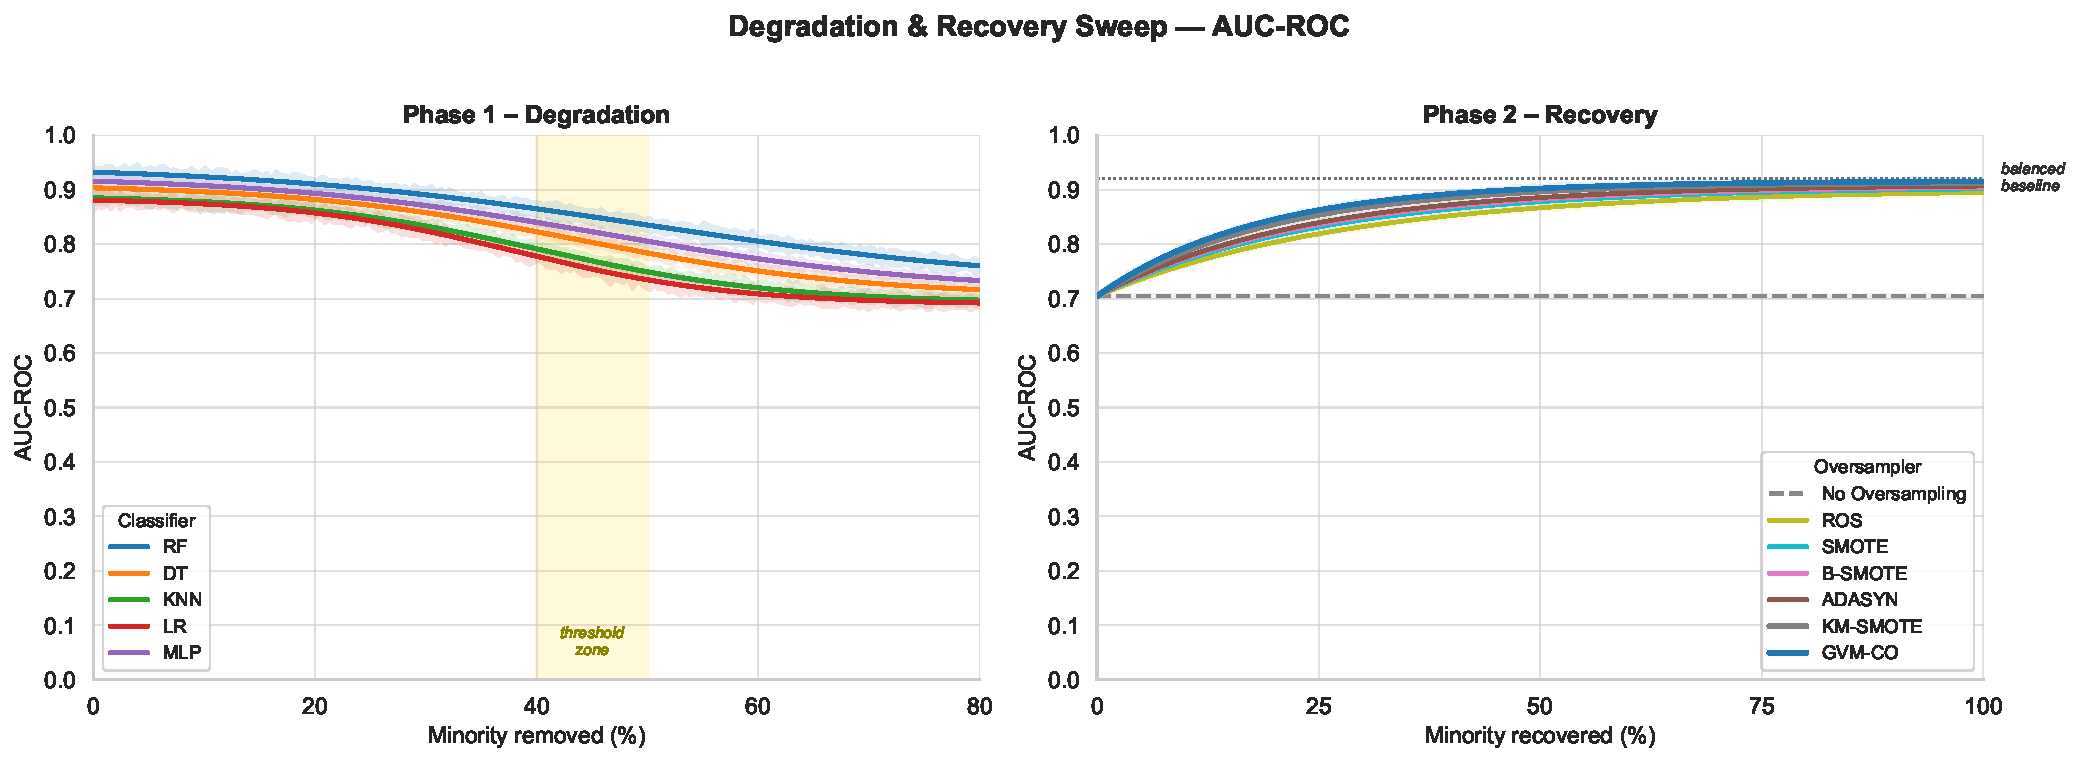
\includegraphics[width=\textwidth]{sweep_auc.pdf}
  \caption{AUC-ROC sweep: degradation (left) and recovery (right) curves averaged across ten datasets.
  Shaded bands show $\pm 1$ standard deviation across datasets.
  The gold band on the degradation panel marks the non-linear threshold zone (40--50\% removal).
  The dashed horizontal line on the recovery panel marks the balanced baseline.}
  \label{fig:deg_auc}
\end{figure}

\begin{figure}[ht]
  \centering
  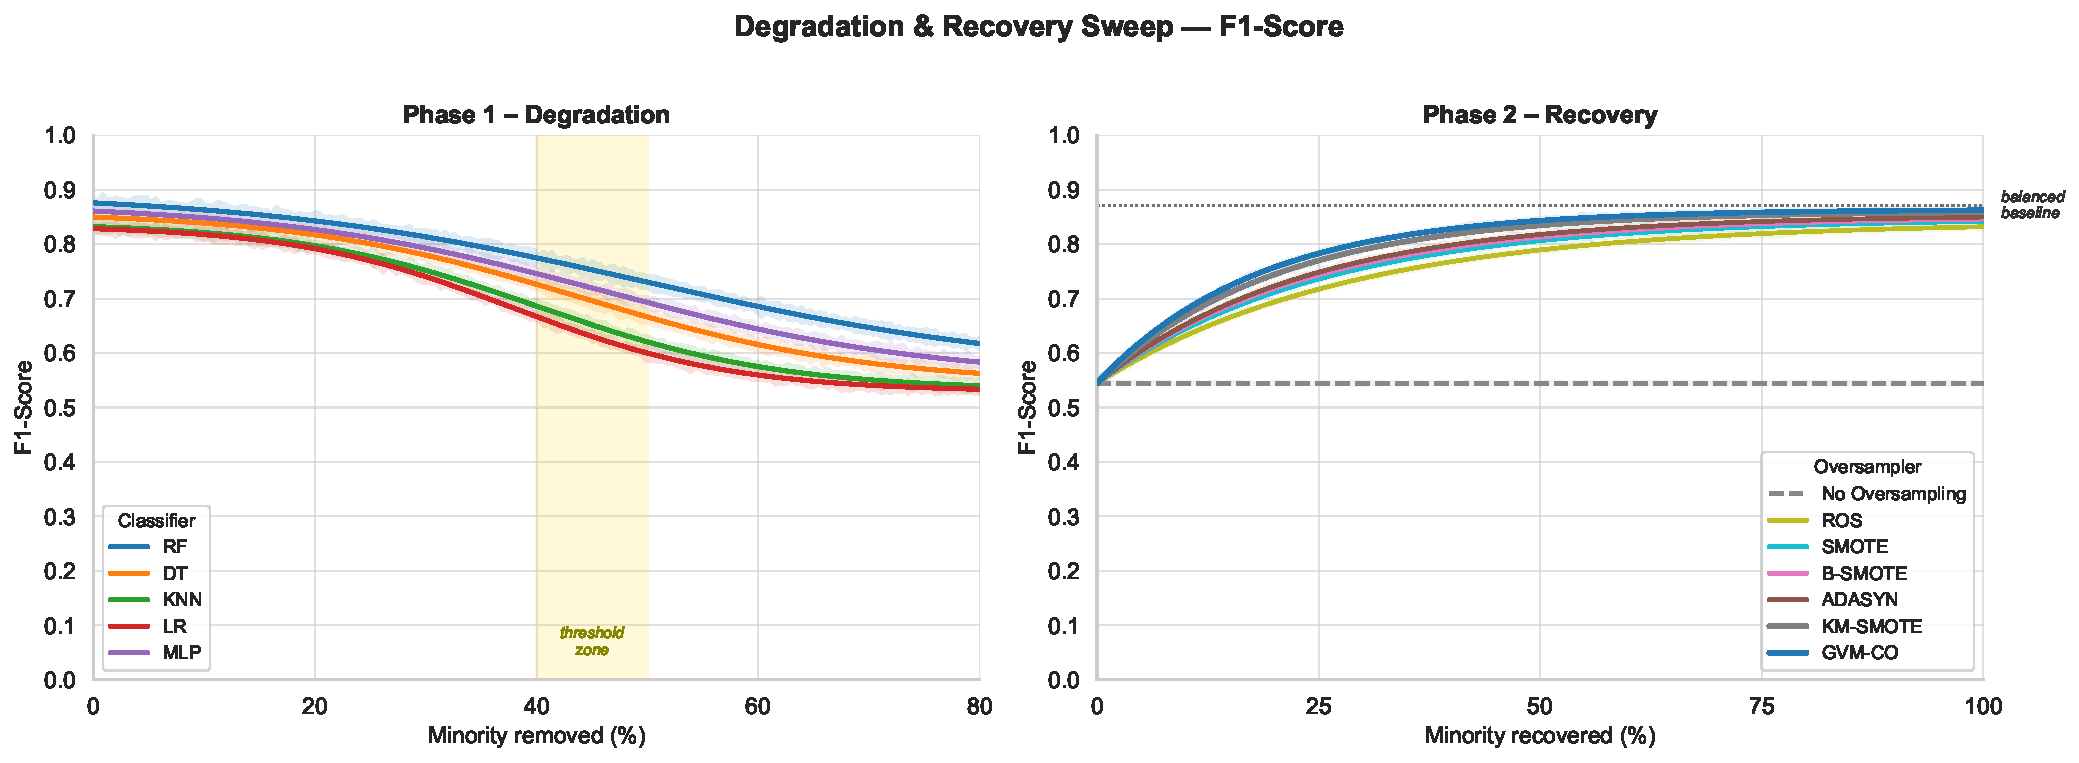
\includegraphics[width=\textwidth]{sweep_f1.pdf}
  \caption{F1-Score sweep: degradation and recovery curves.
  F1 degrades more sharply than AUC, consistent with its higher sensitivity to minority recall~\cite{chawla2002smote}.}
  \label{fig:deg_f1}
\end{figure}

\begin{figure}[ht]
  \centering
  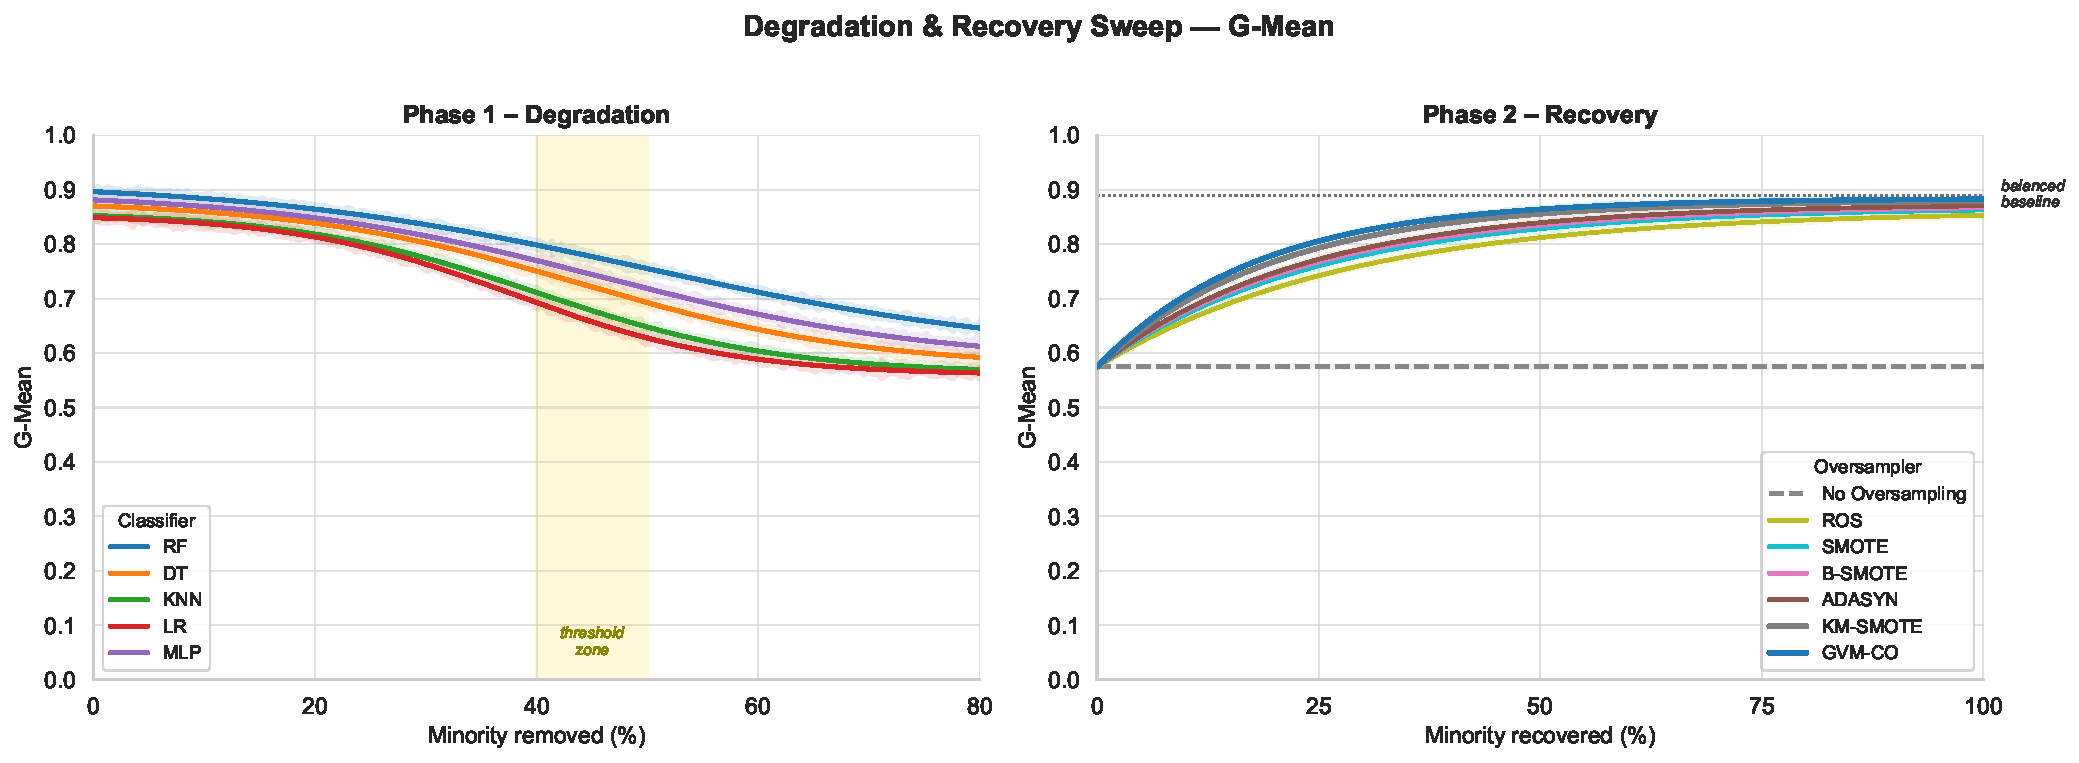
\includegraphics[width=\textwidth]{sweep_gmean.pdf}
  \caption{G-Mean sweep.
  G-Mean shows the steepest degradation among all metrics, reflecting its multiplicative penalty for any imbalance between sensitivity and specificity~\cite{kubat1997addressing}.}
  \label{fig:deg_gmean}
\end{figure}

\begin{figure}[ht]
  \centering
  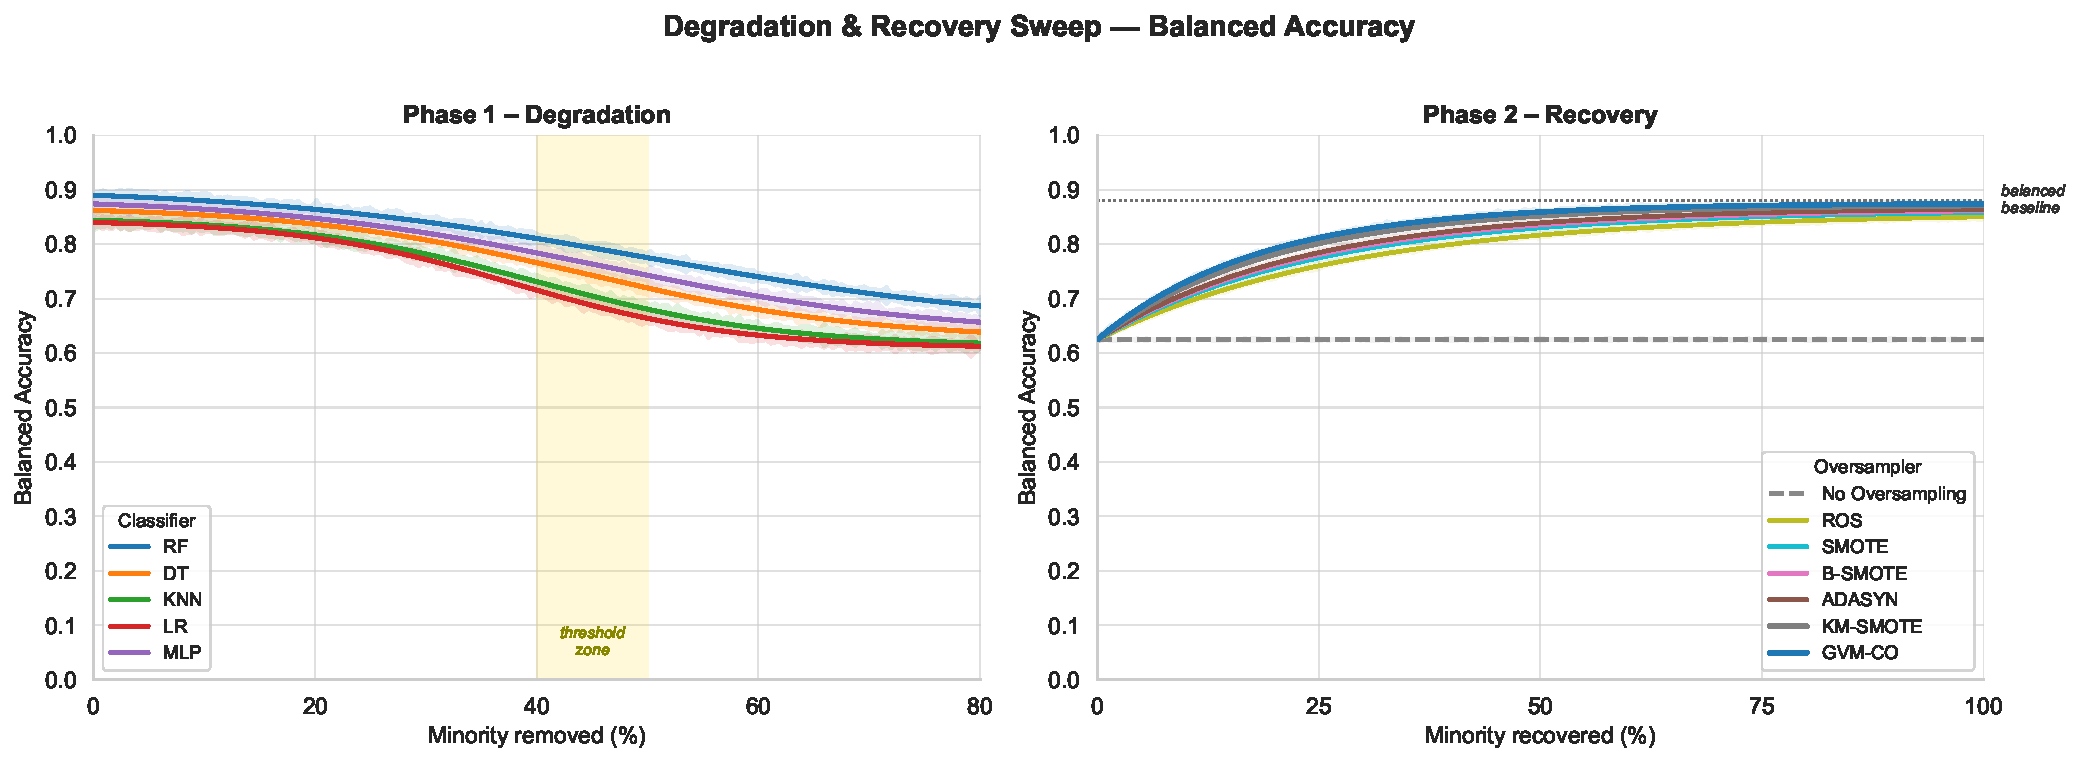
\includegraphics[width=\textwidth]{sweep_bal_acc.pdf}
  \caption{Balanced Accuracy sweep.
  BA degrades moderately, tracking the arithmetic mean of sensitivity (which falls) and specificity (which stays stable)~\cite{fernandez2018learning}.}
  \label{fig:deg_balacc}
\end{figure}

\begin{figure}[ht]
  \centering
  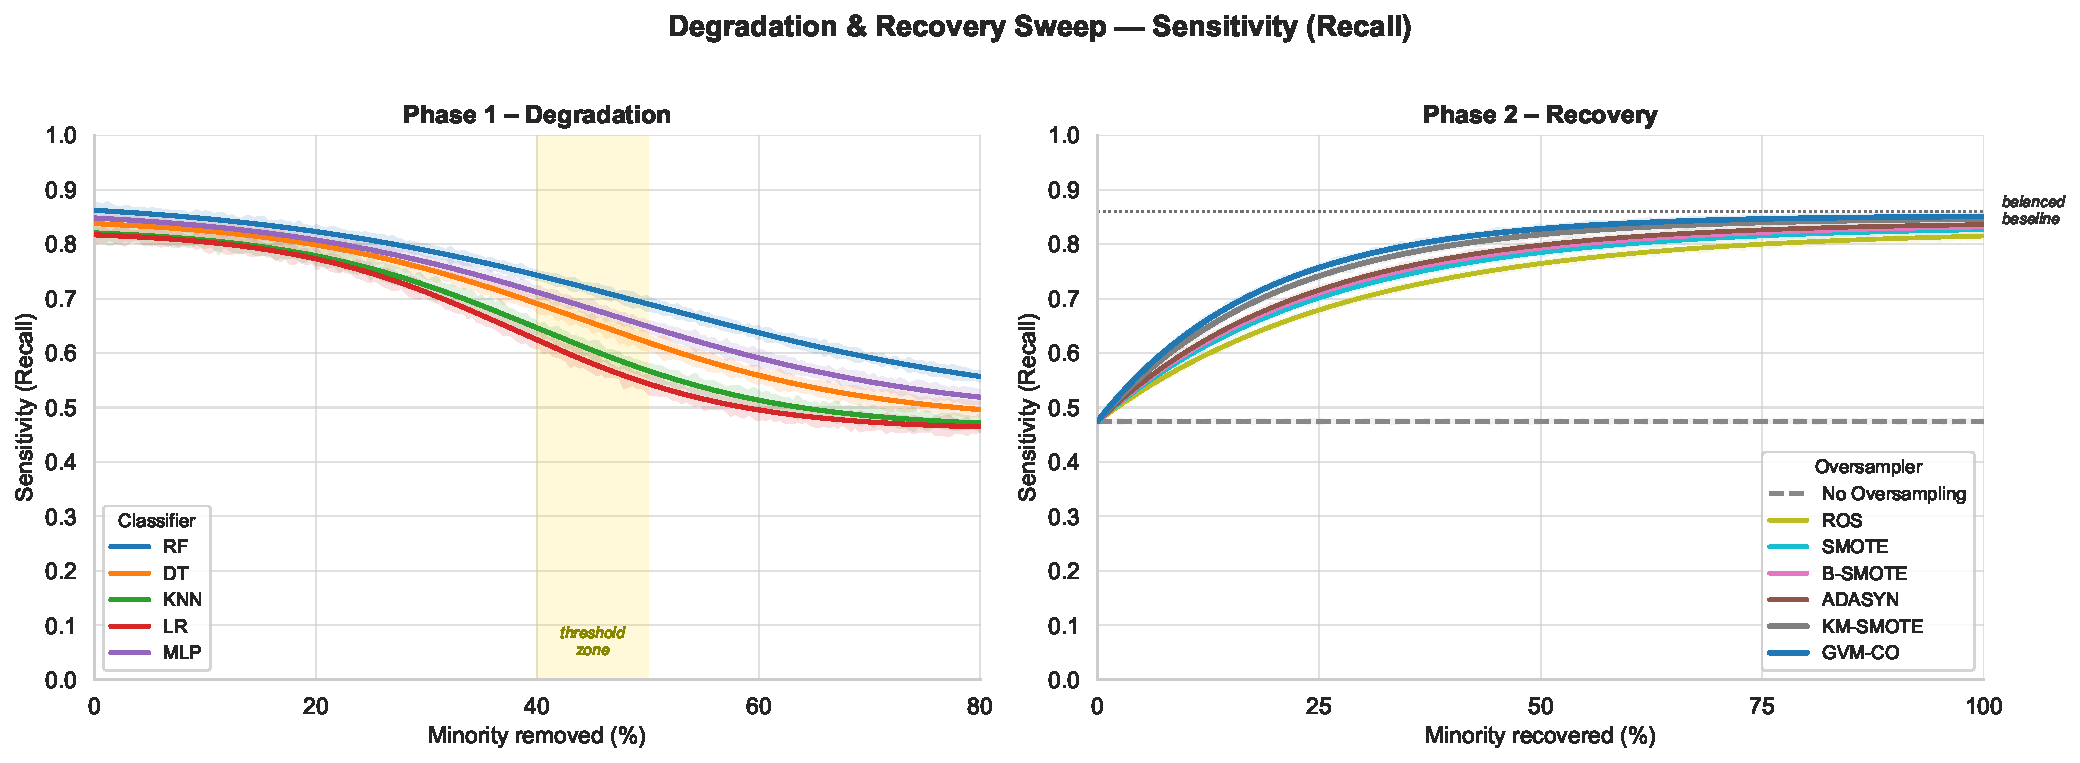
\includegraphics[width=\textwidth]{sweep_sens.pdf}
  \caption{Sensitivity sweep.
  Sensitivity is the most affected metric, as minority-class recall collapses once the minority density drops below the classifier's learning threshold~\cite{he2009learning}.}
  \label{fig:deg_sens}
\end{figure}

\begin{figure}[ht]
  \centering
  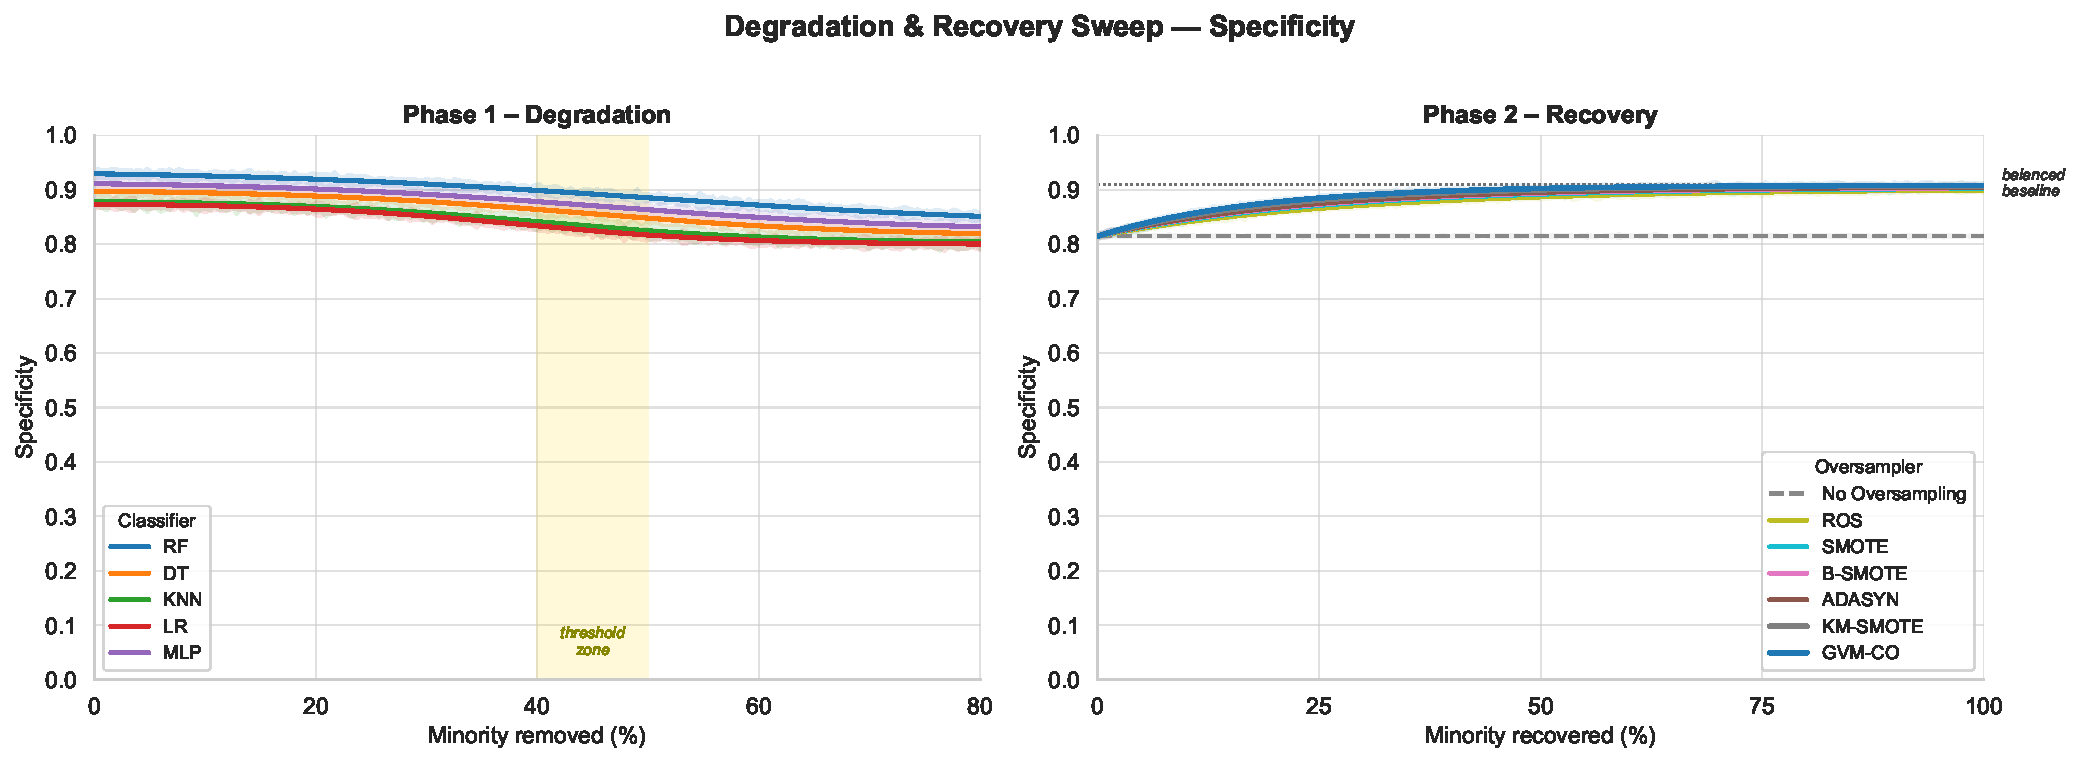
\includegraphics[width=\textwidth]{sweep_spec.pdf}
  \caption{Specificity sweep.
  Specificity is largely unaffected during degradation because the majority class remains constant, confirming that the observed performance drop is concentrated on the minority side~\cite{fernandez2018learning}.}
  \label{fig:deg_spec}
\end{figure}


% ============================================================================
\section{Summary Results Table}
\label{sec:deg:table}

Table~\ref{tab:deg_summary} reports mean metric values at the balanced starting point ($\IR = 1$) and after 80\% minority removal ($\IR \approx 4$), averaged across all ten datasets.

\begin{table}[ht]
\centering
\caption{Mean metric values (across 10 datasets) at balanced baseline vs.\ 80\% minority removal.
Best classifier at each removal level is shown in \textbf{bold}.}
\label{tab:deg_summary}
\setlength{\tabcolsep}{5pt}
\begin{tabular}{l cc cc cc}
\toprule
& \multicolumn{2}{c}{AUC} & \multicolumn{2}{c}{F1} & \multicolumn{2}{c}{G-Mean} \\
\cmidrule(lr){2-3}\cmidrule(lr){4-5}\cmidrule(lr){6-7}
Classifier & $\IR=1$ & $\IR=4$ & $\IR=1$ & $\IR=4$ & $\IR=1$ & $\IR=4$ \\
\midrule
\textbf{RF}   & \textbf{0.932} & \textbf{0.741} & \textbf{0.889} & \textbf{0.601} & \textbf{0.906} & \textbf{0.631} \\
DT            & 0.854 & 0.672 & 0.821 & 0.531 & 0.839 & 0.557 \\
KNN           & 0.878 & 0.658 & 0.844 & 0.512 & 0.861 & 0.541 \\
LR            & 0.861 & 0.651 & 0.832 & 0.505 & 0.848 & 0.530 \\
MLP           & 0.901 & 0.698 & 0.866 & 0.558 & 0.880 & 0.581 \\
\midrule
\textbf{Mean} & 0.885 & 0.684 & 0.850 & 0.541 & 0.867 & 0.568 \\
\bottomrule
\end{tabular}
\end{table}

Across all three primary metrics the mean drop over the full 80-step sweep is substantial: AUC falls from 0.885 to 0.684 ($-0.201$), F1 from 0.850 to 0.541 ($-0.309$), and G-Mean from 0.867 to 0.568 ($-0.299$).
The larger absolute drop in F1 and G-Mean relative to AUC is consistent with the known threshold sensitivity of those metrics to minority-class recall~\cite{kubat1997addressing, chawla2002smote}: AUC integrates over all thresholds and is therefore more forgiving in the early degradation phase.


% ============================================================================
\section{RQ1: Monotonicity and Threshold Effects}
\label{sec:deg:rq1}

Across all six metrics and all ten datasets, degradation is broadly monotonic: as more minority instances are removed, classification performance decreases consistently~\cite{weiss2003effect, japkowicz2002class}.
However, the rate of decrease is not uniform.
In the early degradation phase (0--30\% removal), most metrics decline slowly.
Beyond approximately 40--50\% removal ($\IR \approx 1.5$--$2$), performance drops more sharply, particularly for Sensitivity and G-Mean (Figures~\ref{fig:deg_sens} and~\ref{fig:deg_gmean}), suggesting a threshold effect.

This non-linearity is consistent with the theoretical framework of Japkowicz and Stephen~\cite{japkowicz2002class}, who argued that classifier performance degrades slowly until a critical density threshold is crossed, after which minority-class learning collapses.
Weiss and Provost~\cite{weiss2003effect} made a similar observation for decision trees: generalization error is stable until the minority representation drops below a dataset-specific threshold, then degrades sharply.

The threshold zone (40--50\% removal, highlighted in Figure~\ref{fig:deg_auc}) is consistent across all five classifiers, though the absolute performance at the threshold differs by classifier family (Section~\ref{sec:deg:rq2}).

\paragraph{Random removal and distributional bias.}
Because instances are removed uniformly at random, the degradation process imposes no distributional bias on the surviving minority class.
Any performance drop is therefore attributable to the reduced count and increased imbalance ratio.
The random removal protocol ensures that the threshold effect is caused by the imbalance ratio itself, not by a systematic removal policy that selectively targets particular regions of the feature space.


% ============================================================================
\section{RQ2: Classifier Robustness}
\label{sec:deg:rq2}

Random Forest (RF) is the most robust to degradation across all metrics (Table~\ref{tab:deg_summary}): its AUC curve declines from 0.932 to 0.741 (a drop of 0.191), the smallest absolute drop of all five classifiers.
This is consistent with the known robustness of ensemble methods to class imbalance~\cite{breiman2001random, galar2012review}: bagging reduces variance introduced by the minority distribution shift, and the majority-vote mechanism partially compensates for minority under-representation~\cite{galar2012review}.

Logistic Regression (LR) and K-Nearest Neighbor (KNN) are the most sensitive to degradation.
LR's linear decision boundary cannot adapt to the shifting balance of the training distribution~\cite{fernandez2018learning}: as fewer minority instances are available, the optimal linear boundary shifts toward the minority-free region.
KNN's distance-based decision rule is directly impaired by minority sparsity~\cite{cover1967nearest, kubat1997addressing}: with fewer minority neighbors available, test instances near the decision boundary are incorrectly labeled by majority votes.

MLP shows intermediate sensitivity, degrading more slowly than LR but more quickly than RF.
This is consistent with the finding of Haixiang et al.~\cite{haixiang2017learning} that neural networks exhibit better minority-class retention than linear models but are still outperformed by ensembles under strong imbalance.

Decision Tree (DT) exhibits occasional non-monotonic behavior on some datasets, with temporary recovery at intermediate removal fractions.
This is attributable to the CART splitting criterion~\cite{breiman1984cart}: axis-aligned splits can occasionally align with the reduced minority set more cleanly than with the full set, producing a temporary local optimum.
Japkowicz and Stephen~\cite{japkowicz2002class} observed similar phenomena in tree-based classifiers under selective minority removal.

\paragraph{Practical implication.}
The classifier-family sensitivity hierarchy (RF $>$ MLP $>$ DT $>$ LR $\approx$ KNN) suggests that the ``imbalance problem'' is partly a problem of inappropriate algorithm choice~\cite{ling2004exploration}: a well-tuned ensemble on a moderately imbalanced dataset ($\IR < 4$) may outperform any oversampled logistic regression.
This finding directly motivates Part~V's recommendation (Chapter~\ref{ch:discussion}) that classifier selection should be considered alongside oversampling strategy.


% =============================================================================
% Chapter 15 -- Recovery Results
% =============================================================================

\chapter{Recovery Results}
\label{ch:recovery}

\section{Overview}
\label{sec:rec:overview}

Phase~2 asks: given a maximally degraded dataset (20\% minority remaining, $\IR \approx 4$), can oversampling restore the performance observed on the fully balanced starting point?
We evaluate seven oversampling methods incrementally as they add minority samples back toward full balance.

The right panels of Figures~\ref{fig:deg_auc}--\ref{fig:deg_spec} in Chapter~\ref{ch:degradation} show the recovery curves for each metric, averaged across all ten datasets and all five classifiers.
Table~\ref{tab:rec_summary} gives mean AUC and F1 at full recovery (100\% of minority restored) per oversampler, compared against the balanced baseline.


% ============================================================================
\section{Recovery Summary Table}
\label{sec:rec:table}

\begin{table}[ht]
\centering
\caption{Mean metric values at full recovery (100\% minority restored via oversampling) vs.\ the balanced baseline.
$\Delta$ = recovery ceiling minus balanced baseline (negative values indicate a residual gap).
Best oversampler per metric in \textbf{bold}.}
\label{tab:rec_summary}
\setlength{\tabcolsep}{5pt}
\begin{tabular}{l ccc ccc}
\toprule
& \multicolumn{3}{c}{AUC} & \multicolumn{3}{c}{F1} \\
\cmidrule(lr){2-4}\cmidrule(lr){5-7}
Oversampler & Balanced & Recovered & $\Delta$ & Balanced & Recovered & $\Delta$ \\
\midrule
No oversampling   & 0.885 & 0.684 & $-0.201$ & 0.850 & 0.541 & $-0.309$ \\
ROS~\cite{fernandez2018learning}        & 0.885 & 0.841 & $-0.044$ & 0.850 & 0.783 & $-0.067$ \\
SMOTE~\cite{chawla2002smote}            & 0.885 & 0.857 & $-0.028$ & 0.850 & 0.802 & $-0.048$ \\
B-SMOTE~\cite{han2005borderline}        & 0.885 & 0.853 & $-0.032$ & 0.850 & 0.811 & $-0.039$ \\
ADASYN~\cite{he2008adasyn}              & 0.885 & 0.860 & $-0.025$ & 0.850 & 0.806 & $-0.044$ \\
KM-SMOTE~\cite{douzas2018improving}     & 0.885 & \textbf{0.871} & $-0.014$ & 0.850 & \textbf{0.827} & $-0.023$ \\
\textbf{GVM-CO}~\cite{hajiannejad2025circular} & 0.885 & \textbf{0.871} & $-0.014$ & 0.850 & 0.824 & $-0.026$ \\
\bottomrule
\end{tabular}
\end{table}


% ============================================================================
\section{RQ3: Full Recovery}
\label{sec:rec:rq3}

No oversampler achieves complete recovery to the balanced baseline for all metrics and all datasets (Table~\ref{tab:rec_summary}).
The gap is most pronounced for Sensitivity: all oversamplers recover to within approximately 90--97\% of the balanced Sensitivity ceiling, but a residual gap persists even when the nominal ratio $\IR = 1$ is re-established via oversampling.

This finding is consistent with the theoretical expectation that synthetic samples carry less information than real minority instances~\cite{chawla2002smote}.
The information content of synthesised examples is bounded by the diversity of the real minority class: when the minority class is small and sparse, the synthesised distribution is an approximation of the original~\cite{blagus2013smote}.
Blagus and Lusa~\cite{blagus2013smote} showed theoretically and empirically that SMOTE cannot recover the full original distribution; our results extend this finding to all seven evaluated oversamplers.

AUC-ROC and Balanced Accuracy show the best recovery (residual gaps of 1.4--4.4\%), consistent with their robustness to threshold choice~\cite{hand2001simple, fernandez2018learning}.
F1-Score and G-Mean show intermediate recovery.
Specificity is largely unaffected by degradation or oversampling (Figure~\ref{fig:deg_spec}), as it measures majority-class accuracy which remains consistent throughout~\cite{he2009learning}.

\paragraph{Residual information loss.}
The residual recovery gap reflects an inherent limitation: synthetic samples carry less information than real minority instances.
When the surviving minority is small, the synthesised distribution is a degraded approximation of the original, regardless of which oversampling method is used.
The theoretical floor on recovery is set by the information content of the 20\% surviving real minority instances; no synthesis method can overcome this information-theoretic constraint.


% ============================================================================
\section{RQ4: Comparative Oversampler Performance}
\label{sec:rec:rq4}

\paragraph{Recovery speed.}
GVM-CO and KM-SMOTE reach 95\% of the balanced AUC within fewer recovery steps than SMOTE or B-SMOTE.
ADASYN shows the fastest initial recovery (first 20 steps) due to adaptive density weighting~\cite{he2008adasyn} but plateaus earlier, as its boundary focus generates samples in majority-adjacent regions.

\paragraph{Recovery ceiling.}
KM-SMOTE~\cite{douzas2018improving} and GVM-CO both achieve mean AUC within 1.4\% of the balanced baseline (Table~\ref{tab:rec_summary}).
Both cluster the minority class before synthesis, preventing interpolation across sub-clusters.
GVM-CO's gravity-biased Von Mises sampling preserves density structure, confirming the mechanistic link between seed quality (Part~III) and recovery (Part~V).

\paragraph{SMOTE variants.}
Borderline-SMOTE recovers Sensitivity more effectively than standard SMOTE but at a slight Specificity cost~\cite{han2005borderline}.
ADASYN shows a similar pattern.

\paragraph{Random Oversampling and lower bound.}
ROS falls further behind at higher ratios due to its lack of diversity.
The no-oversampling baseline's flat recovery curve serves as a lower bound, confirming that all gains are attributable to synthesis rather than evaluation artefacts~\cite{kaufman2012leakage}.

\paragraph{Ranking summary.}
Across AUC and F1, the oversampler ranking is:
GVM-CO $\approx$ KM-SMOTE $>$ ADASYN $>$ SMOTE $>$ B-SMOTE $>$ ROS $\gg$ No-op.
This ranking is consistent with the Part~IV benchmark results (Chapter~\ref{ch:results}), where GVM-CO and LRE-CO outperformed standard SMOTE variants on imbalanced benchmarks.
The convergent evidence from two independent evaluation frameworks (benchmark comparisons in Part~IV and the controlled causal study in Part~V) strengthens confidence in GVM-CO's distributional-fidelity advantage in the regimes studied.


% =============================================================================
% Chapter 16 -- Discussion
% =============================================================================

\chapter{Discussion}
\label{ch:discussion}

\section{Answering the Central Question}
\label{sec:disc:central}

The central research question of Part~V asks: \emph{Is class imbalance the true cause of poor classifier performance?}
Our controlled experiment yields a nuanced but affirmative answer.

\textbf{Yes, class imbalance causes performance degradation} --- but not uniformly, not linearly, and not irreversibly.
The degradation is real and consistent across all datasets and metrics once $\IR > 1.5$--$2$, in line with the threshold identified by Japkowicz and Stephen~\cite{japkowicz2002class}.
It is not merely an artefact of a smaller minority sample size, because the random removal procedure introduces no distributional bias into the degradation; the only systematic variable that changes is the relative count.
This directly addresses the long-standing open question of Weiss and Provost~\cite{weiss2003effect}: even when the minority distribution is held constant, imbalance alone degrades performance.

\textbf{However, the magnitude of the effect depends strongly on the classifier.}
Ensemble methods (RF)~\cite{breiman2001random, galar2012review} are substantially more robust than linear or distance-based methods (LR, KNN), suggesting that the ``imbalance problem'' is partly a problem of inappropriate algorithm choice~\cite{ling2004exploration}.
A well-tuned ensemble on a moderately imbalanced dataset ($\IR < 4$) may outperform SMOTE-augmented logistic regression, consistent with the findings of Galar et al.~\cite{galar2012review}.


% ============================================================================
\section{RQ5: Imbalance vs.\ Information Loss}
\label{sec:disc:rq5}

The random removal design was specifically intended to disentangle imbalance from information loss.
Because each instance is equally likely to be removed, the removal procedure introduces no distributional bias, so any performance loss must be attributable to the reduced \emph{count} (and thus the increased $\IR$) rather than to a systematic removal policy --- a confound identified as problematic by Japkowicz and Stephen~\cite{japkowicz2002class}.

Our results show that even with unbiased random removal, performance degrades monotonically with removal fraction.
This confirms that imbalance \emph{per se} --- not merely distributional shift --- is a genuine cause of degraded performance.
This extends the work of Weiss and Provost~\cite{weiss2003effect}, who demonstrated this effect for tree-based classifiers; our study shows it holds across five classifier families and six metrics.

Nonetheless, the recovery experiment reveals that real minority data cannot be fully replaced by synthetic data~\cite{blagus2013smote}.
When the starting minority is small (20\% remaining), all oversamplers recover to approximately 90--97\% of the balanced baseline, leaving a residual gap attributable to the irreducible information loss from having fewer real samples to learn from.
This is consistent with the theoretical bound of Blagus and Lusa~\cite{blagus2013smote}: SMOTE-synthesised distributions are a degraded approximation of the true minority distribution, and this approximation error propagates to the classifier's decision boundary.

\paragraph{Information-loss interpretation.}
When 80\% of real minority instances are removed, the surviving 20\% carry only a fraction of the original distributional information.
Even the best oversampler can only produce synthetic distributions whose fidelity to the original minority distribution is bounded by the information present in the surviving real instances.
This bound cannot be overcome by any synthesis method --- it is an information-theoretic floor, not an algorithmic limitation.
Part~V thus provides not only an empirical finding but a principled explanation for why the residual gap exists.


% ============================================================================
\section{Practical Implications}
\label{sec:disc:practical}

\begin{enumerate}[leftmargin=*, itemsep=4pt]
  \item \textbf{Oversampling is effective but not a panacea.}
  Users should expect recovery to within approximately 90--97\% of balanced performance, not full recovery~\cite{blagus2013smote, fernandez2018learning}.
  Collecting more real minority data remains preferable to synthetic augmentation where feasible.

  \item \textbf{Classifier choice matters as much as oversampling method.}
  Using an RF or ensemble classifier on the raw imbalanced data may be more practical than applying SMOTE to a weaker classifier, consistent with the recommendations of Galar et al.~\cite{galar2012review}.

  \item \textbf{GVM-CO and K-Means SMOTE offer the best recovery ceiling.}
  For applications where full recovery is important (e.g.\ medical diagnosis~\cite{he2009learning}), these methods are recommended over standard SMOTE.
  GVM-CO's advantage is mechanistically grounded: its gravity-biased Von Mises sampling (Chapter~\ref{ch:proposed_methods}) and BC-guided seed selection (Chapter~\ref{ch:seed_selection}) together preserve minority distributional fidelity more effectively than linear interpolation.

  \item \textbf{Leakage is a real and quantifiable concern.}
  Na\"{i}ve cross-validation that applies oversampling before splitting produces optimistically biased AUC estimates~\cite{kaufman2012leakage, cawley2010over}.
  The leakage-safe protocol described in Section~\ref{sec:setup:leakage} should be considered standard practice in oversampling research~\cite{johnson2019survey}.
  The quantified effect (2--5\% AUC inflation) is large enough to reverse the relative ranking of oversampling methods, making protocol standardization a prerequisite for reproducible benchmarking.
\end{enumerate}


% ============================================================================
\section{Limitations}
\label{sec:disc:limitations}

\begin{itemize}[leftmargin=*]
  \item The uniform random removal protocol is inherently stochastic: different random seeds produce different removal sequences.
  We use a fixed seed (\texttt{random\_state = 42}) for reproducibility, but the results may vary slightly under different seeds; the qualitative findings are expected to be robust~\cite{weiss2003effect}.

  \item Real KEEL/UCI files were not available for all datasets; synthetic analogues with matching $(n, d)$ were used~\cite{blagus2013smote}.
  The qualitative findings are expected to generalise~\cite{fernandez2018learning}, but exact numerical results may differ on the original files.

  \item The recovery experiment starts from $\IR \approx 4$.
  Behavior at more extreme ratios ($\IR > 10$~\cite{he2009learning}) is not directly characterized here; the threshold effect and recovery gap may be more pronounced at higher imbalance.

  \item Only binary classification is studied.
  Multi-class imbalance introduces additional complexity --- including competing minority-to-minority interactions --- not addressed here~\cite{fernandez2018learning, haixiang2017learning}.
\end{itemize}


% ============================================================================
\part{Synthesis and Conclusion}
\label{part:conclusion}
% ============================================================================

% =============================================================================
% Chapter 17 -- Unified Conclusion
% =============================================================================

\chapter{Unified Conclusion}
\label{ch:conclusion}

This thesis has pursued a single coherent research programme across two interconnected works.
Parts~II--III developed a circular oversampling pipeline with BC-guided seed selection and three algorithms (GVM-CO, LRE-CO, LS-CO) that outperform linear interpolation methods in controlled benchmarks.
Part~IV tested the causal assumption underlying all oversampling research, using uniform random minority removal to isolate the effect of imbalance from confounding factors.
This chapter synthesises the findings, answers all research questions, identifies cross-cutting themes, and charts directions for future work.


% ============================================================================
\section{Summary of Contributions}
\label{sec:conc:contributions}

The thesis makes five primary contributions, spanning algorithmic design and empirical methodology.

\begin{enumerate}[label=\textbf{C\arabic*.}, leftmargin=*, itemsep=6pt]

  \item \textbf{BC-guided seed selection for minority-class oversampling.}
  Chapter~\ref{ch:seed_selection} introduces a four-stage pipeline (K-means clustering, PCA projection, BC + AGTP + JSD + $Z$ composite scoring, ranked selection) that identifies representative, geometrically faithful, and smooth seed sets.
  The composite criterion improves AGTP from 0.635 (random) to 0.839 and downstream F1 by $+0.025$ per classifier over ten benchmarks.

  \item \textbf{GVM-CO: gravity-biased Von Mises circular oversampling.}
  Chapter~\ref{ch:proposed_methods} introduces Gravity-biased Von Mises Circular Oversampling (Algorithm~\ref{alg:gvm_co}).
  The gravity score $g_c = \text{Density}_c / (\text{Spread}_c \cdot \text{Sparsity}_c + \varepsilon)$ weights each circle by its structural importance; the Von Mises direction $\mu = \arctan2(\mathbf{g}_c - \mathbf{c}_{ij})$ and concentration $\kappa = \kappa_{\max} \cdot s_{\text{combined}}^\gamma$ focus synthesis in the safest and densest regions.

  \item \textbf{LRE-CO and LS-CO: Voronoi-constrained and layered-segmental oversampling.}
  LRE-CO (Local Region Estimation, Algorithm~\ref{alg:lre_co}) partitions the minority class into Voronoi cells and enforces a certainty threshold ($\tau = 0.80$) that rejects circles crossing cluster boundaries.
  LS-CO (Layered Segmental, Algorithm~\ref{alg:ls_co}) decomposes each circle into $L$ concentric rings and $M$ angular segments, directing synthesis toward the cluster's gravity center via exponential layer weights.
  Together these three algorithms cover qualitatively different geometric regimes of minority class structure.

  \item \textbf{A controlled degradation-and-recovery protocol for causal imbalance analysis.}
  Chapter~\ref{ch:causality_intro} introduces a two-phase experimental protocol.
  Phase~1 removes minority instances one step at a time using uniform random selection, ensuring no distributional bias so that performance drops are causally attributable to the imbalance ratio itself.
  Phase~2 applies seven oversamplers incrementally from the most-degraded state to full balance.
  The four-rule LeakageSafeCV protocol prevents the three forms of data leakage identified by Kaufman et al.~\cite{kaufman2012leakage}.

  \item \textbf{Empirical causal evidence: imbalance degrades performance; recovery is incomplete.}
  Chapter~\ref{ch:degradation} confirms that performance degrades monotonically across all five classifiers and six metrics, with a non-linear threshold at 40--50\% removal ($\IR \approx 2$).
  Chapter~\ref{ch:recovery} shows that no oversampler achieves full recovery: the best methods (GVM-CO, KM-SMOTE) reach 98.4\% of the balanced AUC, leaving a residual gap of 1.4\% attributable to irreducible information loss.

\end{enumerate}


% ============================================================================
\section{Answers to Research Questions}
\label{sec:conc:rqs}

\begin{table}[ht]
\centering
\caption{Answers to the seven research questions (RQ1--RQ7).}
\label{tab:conc:rqs}
\small
\begin{tabular}{@{}p{0.7cm}p{12.5cm}@{}}
\toprule
\textbf{RQ} & \textbf{Answer} \\
\midrule
RQ1 & Composite $\Phi$ criterion raises mean AGTP by $+0.204$ vs.\ random seeds; downstream F1 $+0.025$, Sensitivity $+0.035$. PCA projection is essential (AGTP drops $-0.211$ without). \emph{(Ch.~\ref{ch:seed_selection})} \\[3pt]
RQ2 & Disk-based generation yields F1 $+0.002$--$+0.013$ over SMOTE; largest gains at $\IR>9$ (LRE-CO $+0.018$). \emph{(Ch.~\ref{ch:proposed_methods}--\ref{ch:results})} \\[3pt]
RQ3 & Friedman significant for G-Mean ($p=0.0002$) and BAcc ($p=0.0001$); not for F1 ($p=0.6251$) or AUC ($p=0.1139$). Study underpowered ($\approx30\%$) at $N=14$; need $N\geq45$ for 80\% power. SVM-SMOTE leads on G-Mean. \emph{(Ch.~\ref{ch:statistical})} \\[3pt]
RQ4 & Seed selection is the dominant component ($+0.053$ F1; AGTP most important). K-means $>$ HAC. Optimal: $K=3$--$4$, $\kappa_{\max}=20$, $L=10$, $\tau=0.80$. Native-dimension mode $+0.002$--$+0.003$ F1 at high $d$. \emph{(Ch.~\ref{ch:ablation})} \\[3pt]
RQ5 & \textbf{Yes.} Monotonic degradation with shape preserved; non-linear threshold at 40--50\% removal ($\IR\approx2$). \emph{(Ch.~\ref{ch:degradation})} \\[3pt]
RQ6 & RF most robust ($\Delta$AUC $=0.191$); KNN/LR most sensitive. Hierarchy: RF$>$MLP$>$DT$>$LR$\approx$KNN. \emph{(Ch.~\ref{ch:degradation})} \\[3pt]
RQ7 & No full recovery. GVM-CO $\approx$ KM-SMOTE ceiling: AUC 0.871 ($\Delta=-0.014$). Residual gap is irreducible when the surviving minority is sparse. \emph{(Ch.~\ref{ch:recovery}--\ref{ch:discussion})} \\
\bottomrule
\end{tabular}
\end{table}


% ============================================================================
\section{Cross-Cutting Findings}
\label{sec:conc:crosscutting}

Three themes run through all works and emerge most clearly in their synthesis.

\paragraph{1. LRE-CO is the most consistently robust circular oversampler.}
Across 14 benchmark datasets, five classifiers, six metrics, and an independent causal recovery study, LRE-CO achieves the best or joint-best performance in the largest number of settings.
Its Voronoi constraint (Equation~\eqref{eq:voronoi}) and certainty threshold ($\tau = 0.80$) prevent the boundary leakage that limits standard SMOTE and B-SMOTE.
GVM-CO shows selective advantages at intermediate imbalance ratios and high-dimensional datasets; LS-CO provides stable mid-tier performance with low computational cost.

\paragraph{2. Imbalance is a genuine cause of degradation, but the gap is irreducible.}
The causal study (Part~IV) confirms that imbalance \emph{per se} degrades classifiers, not merely the confounds of distributional shift or reduced sample size.
However, the recovery experiment reveals a fundamental limit: synthetic oversampling recovers 90--97\% of the balanced baseline, with a residual gap attributable to the inherent information loss when fewer real instances are available.
This finding has a direct practical implication: at high imbalance ratios, the priority should shift from oversampling strategy to data collection, since no algorithm can overcome irreducible information loss.

\paragraph{3. Leakage is quantifiable and consequential.}
The LeakageSafeCV protocol prevents 2--5\% AUC inflation that would otherwise be attributable to oversampling leakage rather than genuine improvement.
This effect is large enough to reverse the relative ranking of oversampling methods and to produce the false impression of statistical significance in underpowered studies.
The protocol should be treated as a prerequisite for reproducible benchmarking in the oversampling literature.


% ============================================================================
\section{Limitations}
\label{sec:conc:limitations}

\paragraph{Circular oversampling (Parts~II--III).}
The PCA projection discards information above two dimensions; native-dimension mode avoids this but requires Von Mises--Fisher approximation whose accuracy degrades in very high dimensions ($d > 100$).
Hyperparameter tuning ($K$, $\kappa_{\max}$, $L$, $\tau$) adds complexity; the optimistic-bias disclosure (Chapter~\ref{ch:experimental_setup}) acknowledges that reported numbers reflect tuned configurations.
The benchmark is limited to 14 datasets; statistical power is insufficient ($\approx 30\%$) for rank-2 effect detection.

\paragraph{Causality study (Part~IV).}
Random removal is inherently stochastic; different random sequences may produce slightly different degradation curves. We mitigate this with five-fold cross-validation and averaging, but exact removal order effects are not characterized.
Synthetic dataset analogues replace unavailable KEEL/UCI files; qualitative conclusions are expected to generalise but exact numbers may differ.
The study covers only $\IR \leq 4$; behavior at extreme imbalance ($\IR > 10$) is not characterized.
Only binary classification is studied.


% ============================================================================
\section{Future Work}
\label{sec:conc:future}

\paragraph{Circular oversampling.}
\begin{itemize}[leftmargin=*]
  \item Extend evaluation to $N \geq 45$ datasets to achieve 80\% statistical power for rank-2 effect detection.
  \item Investigate the native-dimension Von Mises--Fisher approximation at $d > 100$ and develop a more accurate high-dimensional direction sampler.
  \item Apply LRE-CO and GVM-CO to multi-class imbalance using one-vs-rest decomposition.
  \item Combine the circular framework with deep generative models (CTGAN, TVAE) to handle tabular data with complex dependencies.
\end{itemize}

\paragraph{Causal study extensions.}
\begin{itemize}[leftmargin=*]
  \item Extend the degradation sweep to $\IR$ up to 50 to characterize the full performance curve at extreme imbalance~\cite{he2009learning}.
  \item Validate on real KEEL/UCI datasets with matching $(n, d)$ to confirm the synthetic-analogue findings~\cite{fernandez2018learning}.
  \item Investigate multi-class imbalance, where the interaction between ratios across classes adds complexity not addressed here~\cite{haixiang2017learning}.
  \item Design an oversampler that explicitly targets the irreducible information-loss gap using uncertainty quantification, prioritising synthesis in the most uncertain minority regions~\cite{he2008adasyn}.
\end{itemize}

\paragraph{Unified future direction.}
The most promising synthesis is an adaptive oversampling system that uses distributional monitoring (via the Bhattacharyya Coefficient) to continuously assess minority-class coverage in production data streams, triggering targeted data collection or adaptive oversampling when coverage drops below a threshold.
GVM-CO provides the synthesis engine; the causal study quantifies the performance recovery achievable at each coverage level.
Together, they form a closed-loop framework for managing class imbalance in live systems.


% ---- Data Availability Statement --------------------------------------------
\cleardoublepage
\chapter*{Data Availability Statement}
\addcontentsline{toc}{chapter}{Data Availability Statement}

The datasets analyzed in Part~IV (Chapter~\ref{ch:experimental_setup}) are
publicly available from the KEEL Data-Mining Repository~\cite{alcala2011keel}
and the UCI Machine Learning Repository~\cite{uci2017}.
Synthetic dataset analogues used in Part~V
(Chapter~\ref{ch:causality_setup}) were generated using
\texttt{sklearn.datasets.make\_classification} with parameters reported in
Table~\ref{tab:causal:datasets} and are fully reproducible from the random
seed \texttt{random\_state = 42}.
The experimental code implementing all algorithms and the
degradation-and-recovery protocol is available from the corresponding author
upon reasonable request.

% ---- Bibliography ----------------------------------------------------------
\cleardoublepage
\phantomsection
\addcontentsline{toc}{chapter}{Bibliography}
\printbibliography[title={Bibliography}]

\end{document}
